\documentclass[11pt,letterpaper]{article}

% Compile from the folder containing this file.
% This path works in template/ and in sibling course folders.
% Shared formatting for course notes. Loaded by each course's main.tex.
\usepackage[T1]{fontenc}
\usepackage[utf8]{inputenc}
\usepackage{lmodern}
\linespread{1.15}
\usepackage[margin=1in]{geometry}
\usepackage{amsmath,amssymb,amsthm}
\usepackage{mathtools}
\usepackage{graphicx}
\usepackage{booktabs}
\usepackage{enumitem}
\usepackage{xcolor}
\usepackage{hyperref}
\usepackage{tikz}
\usetikzlibrary{decorations.pathreplacing,positioning}
\usepackage{xparse}
\usepackage{etoolbox}

\hypersetup{colorlinks=true,linkcolor=blue!50!black,urlcolor=blue!50!black}
\setlength{\parindent}{0pt}
\setlength{\parskip}{0.5em}
\setlist{nosep}

% Unnumbered section headings: entries show as "Week 1", not "1 Week 1",
% both in the body and in the table of contents.
\setcounter{secnumdepth}{0}

% Each \section (i.e. each week's entry) starts on its own new page. The
% \newpage that used to follow \tableofcontents in each course's main.tex
% is redundant now and has been removed, so week 1 isn't pushed to a blank
% page by this.
\pretocmd{\section}{\newpage}{}{\errmessage{Failed to patch \string\section}}

% Tracks whether \section was the most recent sectioning/lecture command,
% so a \newlecture immediately following a \section (the usual "week's
% first lecture" case) doesn't also throw in its own \newpage, which would
% otherwise leave a blank page between the two. Set true by \section, and
% cleared by \newlecture whether or not it was true, so it only fires for
% a \newlecture that directly follows a \section (nothing else in between).
\newbool{newlecture@justsection}
\pretocmd{\section}{\booltrue{newlecture@justsection}}{}{\errmessage{Failed to patch \string\section}}

% Custom head format: bold, unparenthesized title, with a \quad gap after
% the number (e.g. "Theorem 3.2  Distribution" instead of "Theorem 3.2
% (Distribution)."), reusing amsthm's usual spacing/punctuation otherwise.
% When a title is given, the body text starts on its own new line below the
% head instead of running inline after it; untitled (auto-numbered-only)
% instances stay inline as usual. Body text is upright (not italic) for all
% six environments. Two variants share this head format but differ in
% end-of-head punctuation: theorem/lemma/proposition/exercise keep a
% trailing period, definition/example drop it (no period after the title).
\makeatletter
\newcommand{\thmpunct}{.}
\newtheoremstyle{boldhead}{}{}{\normalfont}{}{\bfseries}{\thmpunct}{5pt plus 1pt minus 1pt}%
    {\thmname{#1}\thmnumber{\@ifnotempty{#1}{ }#2}\thmnote{\@ifnotempty{#3}{\quad#3}}%
     \@ifnotempty{#3}{\def\thmheadnl{\newline}\thm@headsep\z@skip}{}}
\newtheoremstyle{boldheadnp}{}{}{\normalfont}{}{\bfseries}{}{5pt plus 1pt minus 1pt}%
    {\thmname{#1}\thmnumber{\@ifnotempty{#1}{ }#2}\thmnote{\@ifnotempty{#3}{\quad#3}}%
     \@ifnotempty{#3}{\def\thmheadnl{\newline}\thm@headsep\z@skip}{}}
\makeatother

\theoremstyle{boldhead}
\newtheorem{theorem}{Theorem}
\newtheorem{lemma}[theorem]{Lemma}
\newtheorem{proposition}[theorem]{Proposition}
\newtheorem{corollary}[theorem]{Corollary}
\newtheorem{exercise}[theorem]{Exercise}
\theoremstyle{boldheadnp}
\newtheorem{definition}[theorem]{Def.}
\newtheorem{example}[theorem]{Example}
\theoremstyle{remark}
\newtheorem*{remark}{Remark}

% \begin{theorem}[Title][2.7]: both optional arguments are new on top of
% the environments' usual single bracket. The first argument still behaves
% exactly like plain amsthm's optional title (existing notes using
% \begin{example}[Some Name] etc. are unaffected). The second argument, if
% given, overrides the displayed number (e.g. to match a textbook's own
% numbering) instead of the shared theorem counter's automatic value; the
% counter itself still advances normally, so later auto-numbered
% environments are unaffected too.
\newcommand{\addtitleandnumber}[1]{%
    \csletcs{#1orig}{#1}%
    \csletcs{end#1orig}{end#1}%
    \RenewDocumentEnvironment{#1}{o o}{%
        \IfValueT{##2}{\ifblank{##2}{}{\renewcommand{\thetheorem}{##2}}}%
        \IfValueTF{##1}{\ifblank{##1}{\csname#1orig\endcsname}{\csname#1orig\endcsname[##1]}}{\csname#1orig\endcsname}%
    }{\csname end#1orig\endcsname}%
}
\addtitleandnumber{theorem}
\addtitleandnumber{lemma}
\addtitleandnumber{proposition}
\addtitleandnumber{corollary}
\addtitleandnumber{definition}
\addtitleandnumber{example}
\addtitleandnumber{exercise}

% Common mathematical notation.
\newcommand{\R}{\mathbb{R}}
\newcommand{\N}{\mathbb{N}}
\newcommand{\Z}{\mathbb{Z}}
\newcommand{\E}{\mathbb{E}}
\newcommand{\Prob}{\mathbb{P}}
\DeclareMathOperator{\Var}{Var}
\DeclareMathOperator{\Cov}{Cov}

% \newlecture[title][date]: bold, centered marker for the start of a new
% lecture. Both arguments are optional. Numbering runs continuously across
% the whole document (i.e. across all weeks' entries, not reset per
% \section), so the Nth \newlecture in the course is always "Lecture N".
% Each lecture starts on its own new page, except when it directly follows
% a \section heading (which already started a new page of its own), so the
% two stay together instead of leaving a blank page in between.
\newcounter{lecture}
\renewcommand{\thelecture}{\arabic{lecture}}
% Set \lecturetoctrue in a course's main.tex to list each lecture as a
% top-level table-of-contents entry ("Lecture N: title", or the date when
% untitled), with \subsection headings nested beneath it.
\newif\iflecturetoc
\NewDocumentCommand{\newlecture}{o o}{%
    \stepcounter{lecture}%
    \ifbool{newlecture@justsection}{}{\newpage}%
    \boolfalse{newlecture@justsection}%
    \iflecturetoc
        \phantomsection
        \addcontentsline{toc}{section}{Lecture \thelecture\IfValueTF{#1}{\ifblank{#1}{\IfValueT{#2}{\ifblank{#2}{}{ (#2)}}}{: #1}}{\IfValueT{#2}{\ifblank{#2}{}{ (#2)}}}}%
    \fi
    \par\vspace{1em}
    \begin{center}
        \textbf{\Large Lecture \thelecture\IfValueT{#1}{: #1}}\\[2pt]
        \IfValueT{#2}{\normalsize #2}
    \end{center}
    \vspace{0.5em}%
}

% Handwritten-note-style helpers: red definition labels, blue margin
% annotations, yellow highlights, underlined mini-headers.
\newcommand{\deflabel}[2]{\par\noindent{\color{red!70!black}\textbf{Def #1}}\quad\textbf{#2}\par\nobreak}
\newcommand{\exlabel}[2]{\par\noindent\textbf{Example #1}\quad\textbf{#2}\par\nobreak}
\newcommand{\heading}[1]{\par\noindent{\color{red!70!black}\textbf{#1}}\par}
\newcommand{\header}[1]{\par\vspace{0.5em}\noindent\textbf{#1}\par\vspace{-0.2em}}
\newcommand{\aside}[1]{\ifmmode{\color{blue!55!black}\text{\itshape #1}}\else{\color{blue!55!black}\itshape #1}\fi}
\newcommand{\hly}[1]{\colorbox{yellow!55}{$#1$}}
\newcommand{\hlt}[1]{\colorbox{yellow!55}{#1}}
% \boldmath makes any math the argument switches into (e.g. \rb{$r$}) use
% the bold math version automatically, so callers don't need to manually
% wrap math content in \boldsymbol{}.
\newcommand{\rb}[1]{{\color{red!70!black}\boldmath\textbf{#1}}}
\renewcommand{\b}[1]{\textbf{#1}}
\definecolor{navy}{RGB}{0,32,96}
\newcommand{\dbb}[1]{{\color{navy}\textbf{#1}}}
\newcommand{\db}[1]{{\color{navy}#1}}

% Wider padding inside \boxed{} equations (default \fboxsep is 3pt).
% Scoped to \boxed only, so \colorbox highlights (e.g. \hly) are unaffected.
\let\oldboxed\boxed
\renewcommand{\boxed}[1]{{\setlength{\fboxsep}{10pt}\oldboxed{#1}}}

\usepackage{pdfpages}

% Replace these details for each course.
\newcommand{\coursecode}{ESC384}
\newcommand{\coursename}{Partial Differential Equations}
\newcommand{\term}{Fall 2026}
\newcommand{\studentname}{Bonnie Zhuang}

\title{\coursecode{} --- \coursename\\[0.5em]\large Course Notes}
\author{\studentname}
\date{\term}

% Match STA347: no trailing period after theorem/lemma/etc. titles, and
% list each lecture in the table of contents.
\renewcommand{\thmpunct}{}

\lecturetoctrue
% ESC384-only: list just the lectures in the table of contents, not the
% \subsection headings within them.
\setcounter{tocdepth}{1}

% ESC384-only: theorem-like heads (theorem, lemma, proposition, corollary)
% and definition heads are bold red; examples and remarks stay black.
% (Both shared styles are identical here since \thmpunct is empty, so
% swapping one for the other only changes the colour.)
\makeatletter
\appto\th@boldhead{\thm@headfont{\color{red!70!black}\bfseries}}
\AtBeginEnvironment{definition}{\let\th@boldheadnp\th@boldhead}
\AtBeginEnvironment{nremark}{\let\th@boldhead\th@boldheadnp}
\makeatother

% Numbered remarks ("Remark 3.25  Title"), in the same style as theorems;
% the shared remark environment is unnumbered.
\theoremstyle{boldhead}
\newtheorem{nremark}[theorem]{Remark}
\addtitleandnumber{nremark}

% \lecfig[width]{pdf name}{page}{trim: left bottom right top, in bp}{caption}:
% a figure cropped straight out of the original lecture PDF in lectures/,
% with the source's own figure number written into the caption.
\NewDocumentCommand{\lecfig}{O{0.9\linewidth} m m m m}{%
    \par\begin{center}
        \includegraphics[page=#3,trim=#4,clip,width=#1]{lectures/#2.pdf}\\[2pt]
        {\small #5}
    \end{center}
}

\begin{document}
\maketitle
\tableofcontents
% \tableofcontents counts as a \section, so the first \newlecture would
% otherwise skip its own \newpage and start right under the contents.
\newpage

% Typed transcriptions of the lecture PDFs in lectures/, one entry per lecture.
% !TeX root = ../main.tex

\newlecture[Introduction to PDEs]

\subsection{1.1 Introduction}
Our goal in this lecture is to introduce some of the key concepts that we will revisit throughout this course. We provide a definition of partial differential equations (PDEs) and a few carefully chosen model PDEs. We then discuss several ways to classify PDEs with a particular emphasis on second-order PDEs, which are ubiquitous in science and engineering. We conclude the lecture with examples of PDEs in science and engineering.

\subsection{1.2 Partial differential equations}
We first provide a definition of PDEs:

\begin{definition}[Partial Differential Equation (PDE)][1.1]
    A PDE is an equation that relates an unknown function $u$ and some of its partial derivatives, where the function is defined on an $n$-dimensional spatial domain $\Omega \subset \R^n$ and time interval $I \subset \R$. In general, a PDE can be expressed as
    \[G\left(x_1, \dots, x_n, t, u, \frac{\partial u}{\partial x_1}, \dots, \frac{\partial u}{\partial x_n}, \frac{\partial u}{\partial t}, \frac{\partial^2 u}{\partial x_1^2}, \frac{\partial^2 u}{\partial x_1 x_2}, \dots\right) = 0,\]
    where $x_1, \cdots, x_n$ are the spatial coordinates, $t$ is the time, and $\frac{\partial u}{\partial x_1}, \dots$ denote the partial derivatives.
\end{definition}

We provide a few concrete examples of model PDEs that we will study throughout this course:
\begin{itemize}
    \item \textbf{Laplace's equation.} Laplace's equation is given by
    \[-\Delta u = 0,\]
    where $-\Delta = -\nabla \cdot \nabla = -\frac{\partial^2}{\partial x_1^2} - \cdots - \frac{\partial^2}{\partial x_n^2}$ is the Laplacian (under the positive Laplacian convention). Laplace's equation describes various physical phenomena including, but not limited to, the following: steady heat transfer (without a heat source), where $u$ is the temperature; electrostatics, where $u$ is the electrostatic potential; and steady, inviscid, incompressible, irrotational flow, where $u$ is the velocity potential.
    \item \textbf{Poisson's equation.} Poisson's equation is given by
    \[-\Delta u = f,\]
    where $f$ is a source function. Poisson's equation describes the following: steady heat transfer in the presence of a heat source; and electrostatic potential in the presence of charge. Laplace's equation is a special case of Poisson's equation for $f = 0$.
    \item \textbf{Heat equation.} The heat equation is given by
    \[\frac{\partial u}{\partial t} - \nabla \cdot (a \nabla u) = f,\]
    where $a$ is the diffusivity constant, and $f$ is the source term. The heat equation describes the following: unsteady heat transfer; and the diffusion of chemical species.
    \item \textbf{Transport equation.} The transport equation is given by
    \[\frac{\partial u}{\partial t} + b \cdot \nabla u = 0,\]
    where $b$ is an advection field. The transport equation describes the transport of a conserved quantity (e.g., concentration of chemical species) in the presence of an advection field.
    \item \textbf{Wave equation.} The wave equation is given by
    \[\frac{\partial^2 u}{\partial t^2} - c^2 \Delta u = 0,\]
    where $c$ is the wave propagation speed. The wave equation describes the propagation of waves through a medium, including the following: the propagation of acoustic pressure waves in air; the propagation of electromagnetic fields through space; and the vibration of taut strings and membranes.
    \item \textbf{Burgers' equation.} The inviscid Burgers' equation is given by
    \[\frac{\partial u}{\partial t} + u \frac{\partial u}{\partial x} = 0.\]
    Burgers' equation describes the propagation of a nonlinear wave, in which the speed of propagation depends on the solution value. The equation models features such as shocks and rarefaction waves that are encountered in compressible flows.
\end{itemize}

\subsection{1.3 Classification of PDEs}
To facilitate our study of PDEs, we now classify PDEs by a few of their attributes. For each definition that we introduce, we provide a few concrete examples.

\begin{definition}[Order of a PDE][1.2]
    The \textbf{order} of a PDE is the order of the highest-order derivative that appears in the PDE.
\end{definition}

\begin{example}[][1.3]
    Laplace's equation $-\Delta u = 0$ is a second-order PDE, and the transport equation $\frac{\partial u}{\partial t} + a \frac{\partial u}{\partial x} = 0$ is a first-order PDE.
\end{example}

\begin{example}[][1.4]
    The heat equation $\frac{\partial u}{\partial t} - \Delta u = 0$ is a second-order PDE. More precisely, it is first-order in time and second-order in space. Note that time-dependent PDEs admit a more precise characterization.
\end{example}

\begin{definition}[Linear Operator][1.5]
    An operator $\mathcal{L}$ is a \textbf{linear operator} if
    \[\mathcal{L}(\alpha w + \beta v) = \alpha \mathcal{L} w + \beta \mathcal{L} v\]
    for any functions $w$ and $v$ and any scalars $\alpha$ and $\beta$.
\end{definition}

\begin{definition}[Linear PDEs][1.6]
    A PDE is said to be \textbf{linear} if the PDE can be expressed as
    \[\mathcal{L} u = f,\]
    where $\mathcal{L}$ is a linear operator and $f$ is a function independent of $u$. If a PDE is not linear, then it is called a \textbf{nonlinear} PDE.
\end{definition}

\begin{definition}[Linear Homogeneous PDEs][1.7]
    A \textbf{linear homogeneous} PDE is a PDE of the form
    \[\mathcal{L} u = 0,\]
    where $\mathcal{L}$ is a linear operator; i.e., the term independent of $u$ vanishes. If a linear PDE is not homogeneous, then it is \textbf{nonhomogeneous} (or inhomogeneous).
\end{definition}

\begin{example}[][1.8]
    Laplace's equation $-\Delta u = 0$ is a linear homogeneous PDE; the Laplacian $\mathcal{L} \equiv -\Delta$ is a linear operator, and the right hand side is zero. Poisson's equation $-\Delta u = f$ is a linear nonhomogeneous PDE for $f \neq 0$. The heat equation $\frac{\partial u}{\partial t} - \nabla \cdot a \nabla u = f$ is a linear homogeneous PDE if $f = 0$ and is a linear nonhomogeneous PDE if $f \neq 0$. The Burgers' equation $\frac{\partial u}{\partial t} + u \frac{\partial u}{\partial x} = 0$ is a nonlinear PDE, as there is no way to express $u \frac{\partial u}{\partial x}$ as a linear operator on $u$.
\end{example}

\header{The superposition principle.}
Linear homogeneous PDEs, just like linear homogeneous ODEs, are particularly nice to study because we can appeal to the superposition principle to seek a solution. Specifically, if $u_1$ and $u_2$ satisfy $\mathcal{L} u_1 = 0$ and $\mathcal{L} u_2 = 0$, then $u_1 + u_2$ satisfies $\mathcal{L}(u_1 + u_2) = 0$. If, in addition, we find a solution $u_0$ to a nonhomogeneous PDE $\mathcal{L} u_0 = f$, then $u_0 + u_1 + u_2$ also satisfies the nonhomogeneous PDE $\mathcal{L}(u_0 + u_1 + u_2) = f$. We will exploit these properties in many solution techniques throughout this course.

Due to the superposition principle, in general there are infinitely many functions that satisfy a given PDE. We must supply additional conditions to find a unique solution. In the context of PDEs, these conditions are provided by boundary conditions, if the problem is posed in a bounded domain, and by initial conditions, if the problem is time-dependent. (Initial conditions can be thought of as ``boundary conditions'' in the space-time domain.) We will study various boundary and initial conditions for each model PDE in later lectures.

\subsection{1.4 Classification of second-order PDEs}
We have introduced a few second-order linear PDEs including Laplace's equation, the heat equation, and the wave equation. In fact, second-order PDEs are ubiquitous in science and engineering, which justifies a finer classification of these PDEs.

\begin{definition}[Classification of Second-Order Linear PDEs][1.9]
    Consider a second-order linear PDE with a differential operator on $\R^n$:
    \begin{equation*}
        \mathcal{L} u = \sum_{i,j=1}^{n} a_{ij} \frac{\partial^2 u}{\partial x_i \partial x_j} + \sum_{i=1}^{n} b_i \frac{\partial u}{\partial x_i} + cu \tag{1.1}
    \end{equation*}
    for some coefficients $a_{ij}$, $b_i$, and $c$. Let $A \in \R^{n \times n}$ be a symmetric matrix such that $A_{ij} = a_{ij}$, $i, j = 1, \dots, n$. (Note that $A$ can always be symmetrized without loss of generality since the mixed partials are the same.) Let $\lambda_1, \dots, \lambda_n$ be the eigenvalues of $A$. Then we have the following classification of PDEs:
    \begin{itemize}
        \item \textit{elliptic:} all eigenvalues are nonzero and have the same sign (i.e., all positive or all negative).
        \item \textit{hyperbolic:} all eigenvalues are nonzero, and one of them has the opposite sign from the $n-1$ others.
        \item \textit{ultrahyperbolic:} all eigenvalues are nonzero, and at least two of them are positive and at least two of them are negative.
        \item \textit{parabolic:} exactly one eigenvalue is zero and all other eigenvalues have the same sign.
    \end{itemize}
    If the PDE is time-dependent, then we treat time as the zeroth coordinate and run the summations from $0$ to $n$ in (1.1).
\end{definition}

\begin{example}[Classification: Laplace's Equation][1.10]
    The differential operator for Laplace's equation in $\R^n$ is
    \[\mathcal{L} = -\Delta = -\frac{\partial^2}{\partial x_1^2} - \cdots - \frac{\partial^2}{\partial x_n^2}.\]
    We recognize that the associated matrix $A$ is $A = -I$. All eigenvalues are equal to $-1$, and hence Laplace's equation is elliptic.
\end{example}

\begin{example}[Classification: Poisson's Equation][1.11]
    Poisson's equation is also elliptic because its differential operator is the Laplacian.
\end{example}

\begin{example}[Classification: Wave Equation][1.12]
    The differential operator for the wave equation in $\R^n$ is
    \[\mathcal{L} = \frac{\partial^2}{\partial t^2} - \Delta = \frac{\partial^2}{\partial t^2} - \frac{\partial^2}{\partial x_1^2} - \cdots - \frac{\partial^2}{\partial x_n^2}.\]
    We treat the temporal coordinate as the zeroth coordinate and recognize the associated $A$ matrix is $A = \operatorname{diag}(1, -1, -1, \dots, -1) \in \R^{(n+1) \times (n+1)}$. We have one positive eigenvalue and $n$ negative eigenvalues. Hence, the wave equation is hyperbolic.
\end{example}

\begin{example}[Classification: Heat Equation][1.13]
    The differential operator for the heat equation in $\R^n$ is
    \[\mathcal{L} = \frac{\partial}{\partial t} - \Delta = \frac{\partial}{\partial t} - \frac{\partial^2}{\partial x_1^2} - \cdots - \frac{\partial^2}{\partial x_n^2}\]
    We treat the temporal coordinate as the zeroth coordinate and recognize the associated $A$ matrix is $A = \operatorname{diag}(0, -1, -1, \dots, -1) \in \R^{(n+1) \times (n+1)}$. Note that the entry of $A$ associated with the temporal coordinate is $0$ because the differential operator does not contain a second derivative with respect to time. We have one zero eigenvalue and $n - 1$ negative eigenvalues. Hence, the heat equation is parabolic.
\end{example}

\begin{example}[Classification: Finding the $A$ Matrix][1.14]
    Consider a second-order PDE
    \[\frac{\partial^2 u}{\partial x_1^2} - 2 \frac{\partial^2 u}{\partial x_1 \partial x_2} + 2 \frac{\partial^2 u}{\partial x_2^2} = f\]
    for some $f$. We note that the linear differential operator can be rearranged into the form (1.1):
    \[\mathcal{L} u = 1 \frac{\partial^2 u}{\partial x_1^2} - 1 \frac{\partial^2 u}{\partial x_1 \partial x_2} - 1 \frac{\partial^2 u}{\partial x_2 \partial x_1} + 2 \frac{\partial^2 u}{\partial x_2^2},\]
    where we have split the mixed partial term into two so that the coefficients in front of the terms are the same. We recognize that $a_{11} = 1$, $a_{12} = a_{21} = -1$, and $a_{22} = 2$, and hence
    \[A = \begin{pmatrix} 1 & -1 \\ -1 & 2 \end{pmatrix}.\]
    Note that the matrix is symmetric (as required for classification) thanks to the splitting of the mixed partial term. To find the eigenvalues, we form the characteristic equation $p_A(\lambda) \equiv \det(\lambda I - A) = \lambda^2 - 3\lambda + 1$ and find that its roots are $\lambda = \frac{3}{2} \pm \frac{\sqrt{5}}{2}$. Since both eigenvalues are positive, the equation is elliptic.
\end{example}

\begin{example}[Classification: PDE with Variable Coefficient][1.15]
    For PDEs with variable coefficients, the classification may vary over the domain. For instance, consider the second-order PDE
    \[y \frac{\partial^2 u}{\partial x^2} + \frac{\partial^2 u}{\partial y^2} = 0.\]
    The matrix $A$ associated with the PDE is $A = \operatorname{diag}(y, 1)$, and its eigenvalues are $\lambda_1 = 1$ and $\lambda_2 = y$. Hence, the PDE is parabolic on the line $y = 0$, elliptic in the region $y > 0$, and hyperbolic in the region $y < 0$.
\end{example}

The classification of PDEs into elliptic, hyperbolic, and parabolic equations is useful because equations in a given class exhibit similar behaviors. For instance, the only difference between the wave equation (in spacetime, with time as the zeroth coordinate) and Laplace's equation is that one of the eigenvalues is positive in the wave equation; however, the wave equation is hyperbolic and Laplace's equation is elliptic, and they describe different physical processes and exhibit different solution behaviors. On the other hand, while Laplace's equation and the Navier--Cauchy equation of linear elasticity might look quite different, they are both elliptic and exhibit similar behaviors. Similarly, while the wave equation and Maxwell's equations might look quite different, they are both hyperbolic and exhibit similar behaviors.

\subsection{1.5 PDEs in physics and engineering}
Before we conclude this lecture, we provide some examples of more complex PDEs that are encountered in science and engineering. While we will not study these PDEs in detail, we will see that much of the behavior of these more complex PDEs is captured by our model PDEs.
\begin{itemize}
    \item \textbf{Navier--Cauchy equations.} The Navier--Cauchy equations are a system of PDEs of the form
    \[\mu \sum_{j=1}^{d} \frac{\partial^2 u_i}{\partial x_j^2} + (\mu + \lambda) \sum_{j=1}^{d} \frac{\partial^2 u_j}{\partial x_i \partial x_j} = f_i, \quad i = 1, \dots, d,\]
    where $u$ is the (vector-valued) displacement field, $f$ is the body force, and $\lambda$ and $\mu$ are the first and second Lam\'e parameters, respectively. The Navier--Cauchy equations, also known as the equations of linear elasticity, are a system of linear PDEs. The equations describe the deformation of a material under load (under the assumption of small displacements and strains), and hence the behavior of engineering structures.
    \item \textbf{Maxwell's equations.} Maxwell's equations in free space are given by
    \begin{align*}
        \nabla \times E &= -\frac{\partial B}{\partial t}, \\
        \nabla \cdot E &= 0, \\
        \nabla \times B &= \frac{1}{c^2} \frac{\partial E}{\partial t}, \\
        \nabla \cdot B &= 0,
    \end{align*}
    where $E$ is the electric field, $B$ is the magnetic field, and $c$ is the speed of light. Maxwell's equations are a system of linear, homogeneous PDEs. Maxwell's equations describe the propagation of electromagnetic waves in free space, and hence the behavior of electric circuits, electric motors, wireless communication, and power generation, among others.
    \item \textbf{Incompressible Navier--Stokes equations.} The incompressible Navier--Stokes equations are given by
    \begin{align*}
        \frac{\partial u}{\partial t} + \nabla \cdot (u \otimes u) + \nabla p - \frac{1}{\mathrm{Re}} \Delta u &= f, \\
        \nabla \cdot u &= 0,
    \end{align*}
    where $u$ is the (vector-valued) velocity field, $p$ is the (scalar-valued) pressure field, and $\mathrm{Re}$ is the Reynolds number. The incompressible Navier--Stokes equations comprise a system of nonlinear PDEs that describe the velocity and pressure of an incompressible (Newtonian) flow.
    \item \textbf{Compressible Euler equations.} The compressible Euler equations are given by
    \begin{align*}
        \frac{\partial \rho}{\partial t} + \nabla \cdot \rho u &= 0 \\
        \frac{\partial \rho u}{\partial t} + \nabla \cdot (\rho u \otimes u) + \nabla p &= 0 \\
        \frac{\partial \rho e}{\partial t} + \nabla \cdot (\rho h u) &= 0,
    \end{align*}
    where $\rho$ is the density field, $u$ is the (vector-valued) velocity field, $e$ is the specific total energy field, $p$ is the pressure field, and $h$ is the specific enthalpy field. The compressible Euler equations form a system of nonlinear PDEs that describes the behavior of inviscid compressible flows.
    \item \textbf{Schr\"odinger equation.} The Schr\"odinger equation for a single particle is given by
    \[i\hbar \frac{\partial \Psi}{\partial t} = \left(-\frac{\hbar^2}{2m} \Delta + V\right) \Psi,\]
    where $\Psi : \R^n \times \R \to \mathbb{C}$ is the wave function in position space, $\hbar$ is the reduced Planck constant, $m$ is the particle mass, and $V : \R^n \times \R \to \mathbb{C}$ is the potential function. The Schr\"odinger equation describes the quantum state of an isolated nonrelativistic quantum system.
    \item \textbf{Black--Scholes equation.} The Black--Scholes equation is given by
    \[\frac{\partial V}{\partial t} + \frac{1}{2} \sigma^2 S^2 \frac{\partial^2 V}{\partial S^2} + rS \frac{\partial V}{\partial S} - rV = 0,\]
    where $V$ is the price of the option as a function of the stock price $S$ and time $t$, $r$ is the risk-free interest rate, and $\sigma$ is the volatility of the stock.
\end{itemize}

\subsection{1.6 Summary}
We summarize key points of this lecture:
\begin{enumerate}
    \item A PDE is an equation that relates an unknown function $u$ and some of its partial derivatives.
    \item PDEs can be classified in terms of order, linearity, and homogeneity.
    \item PDEs are augmented by initial and/or boundary conditions to provide a well-posed problem.
    \item Second-order PDEs can be further classified as elliptic, hyperbolic, ultrahyperbolic, or parabolic. The classification is based on the eigenvalues of the coefficient matrix of the second-derivative terms.
    \item Laplace's equation, Poisson's equation, the heat equation, the transport equation, the wave equation, and Burgers' equation each serves as a model PDE of a given classification and will be closely studied throughout this course.
\end{enumerate}

\subsection{1.A Well-posedness of a problem}
Throughout this course, we will introduce different techniques to solve PDEs. However, it only makes sense to seek a solution if the problem is \textit{well-posed}. We study this notion in this appendix.

\begin{definition}[Well-Posedness in the Sense of Hadamard][1.16]
    A mathematical problem is said to be \textbf{well-posed} if (i) a solution exists, (ii) the solution is unique, and (iii) the solution depends continuously on the data. If the problem is not well-posed, it is said to be \textbf{ill-posed}.
\end{definition}

As we are not yet equipped to study the well-posedness of PDEs, we consider a few examples of well-posedness in the context of linear algebra and ODEs.

\begin{example}[Linear Algebra][1.17]
    Consider the solution of a linear system associated with a matrix $A \in \R^{n \times n}$: find $x \in \R^n$ such that
    \[Ax = b\]
    for some data $b \in \R^n$. We recall that the problem has a unique solution for any data $b$ if $A$ is nonsingular. In addition, we can readily show that if $Ax_1 = b_1$ and $Ax_2 = b_2$, then $\|x_1 - x_2\| \leq (1/\sigma_{\min}(A)) \|b_1 - b_2\|$, where $\sigma_{\min}(A)$ is the minimum singular value of $A$, which is nonzero for a nonsingular $A$. A small perturbation in the data $b$ results in a small perturbation in the solution $x$. Hence the problem is well-posed if $A$ is nonsingular.

    On the other hand, if $A$ is singular and $b \notin \operatorname{Img}(A)$, then the solution does not exist. If $A$ is singular and $b \in \operatorname{Img}(A)$, then there are infinitely many solutions; if $Ax = b$, then $x + y$ is also a solution for any $y \in \operatorname{Ker}(A)$. (Recall that $\operatorname{Ker}(A) = \{0\}$ for a nonsingular $A$, but $\operatorname{Ker}(A)$ includes other elements for a singular $A$.) Hence, if $A$ is singular, then the problem is ill-posed.
\end{example}

\begin{example}[Initial Value Problem][1.18]
    Consider an initial value problem on $I \equiv (0, T]$ for the final time $T \in \R_{>0}$:
    \begin{align*}
        \frac{du}{dt} &= f(t, u) \quad \text{in } I, \\
        u(t = 0) &= g,
    \end{align*}
    where $u : I \to \R$ is the solution, $f : I \times \R \to \R$ defines the ODE, and $g \in \R$ is the initial condition. Suppose $f$ is continuous in $t$ and uniformly Lipschitz continuous in $u$; i.e., there exists $\gamma < \infty$ such that for any $(t, u_1)$ and $(t, u_2)$ we have $|f(t, u_1) - f(t, u_2)| \leq \gamma |u_1 - u_2|$. Then the Picard--Lindel\"of theorem states that a unique solution to the initial value problem exists. In addition, the energy estimate states that $|u_1(t) - u_2(t)| \leq |g_1 - g_2| \exp(\gamma t)$, which means that the solution depends continuously on the data. Hence the problem is well-posed if the assumptions of the Picard--Lindel\"of theorem hold.

    It is also relatively simple to find $f$ for which the problem is ill-posed. A classical example is
    \begin{align*}
        \frac{du}{dt} &= u^{1/3} \\
        u(t = 0) &= 0;
    \end{align*}
    this initial value problem admits infinitely many solutions of the form
    \[u(t) = \begin{cases} 0, & t \in (0, \tau), \\ \left(\frac{2}{3}(t - \tau)\right)^{3/2}, & t \in (\tau, T], \end{cases}\]
    for any $\tau \in I$. We readily verify that $f(t, u) = u^{1/3}$ does not satisfy the uniform Lipschitz continuity condition of the Picard--Lindel\"of theorem.
\end{example}

% !TeX root = ../main.tex

\newlecture[Fourier Series: Formulation]

\subsection{2.1 Introduction}
In order to solve a PDE, we must be able to represent its solution, which is a function in space (and time). We could attempt to describe the function in terms of the value that it takes at each point in space (and time), but this representation is not convenient for solving or analyzing PDEs. A much more convenient approach is to represent the function as a linear combination of known functions, so that the function can be identified by a set of coefficients. Namely, we represent the solution $u : \Omega \to \R$ as $u(x) = \sum_{n=1}^{\infty} \hat{u}_n \phi_n(x)$, where $\phi_n$, $n = 1, 2, \dots$, are the known functions and $\hat{u}_n$, $n = 1, 2, \dots$, are the coefficients to be determined. One class of infinite series that is particularly useful for representing solutions of PDEs is \textit{Fourier series}. In this lecture, we introduce Fourier series so that we can use them to solve PDEs in the following lectures. In this lecture, we focus on the construction of Fourier series; we will analyze their theoretical properties in the next lecture.

\subsection{2.2 Periodic, even, and odd functions}
As periodic functions play an important role in the construction of Fourier series, we first provide a few definitions related to the periodicity of functions.

\begin{definition}[Periodic Function][2.1]
    A function $f : \R \to \R$ is said to be \textbf{$z$-periodic} if
    \[f(x + z) = f(x) \quad \forall x \in \R.\]
    The real number $z$ is called a \textit{period}. The smallest positive real number $z$ such that the relationship holds is called the \textit{fundamental period}.
\end{definition}

\begin{example}[Periodicity of Sine Functions][2.2]
    Perhaps one of the most common periodic functions is the sine function. The function $f(x) = \sin(x)$ is $2\pi$-periodic because
    \[\sin(x + 2\pi) = \sin(x) \quad \forall x \in \R.\]
    Its fundamental period is $2\pi$, because the relationship does not hold for any shorter period. Note that any integer multiple of the fundamental period is also a period of the function; e.g., $z = 2\pi, 4\pi, 6\pi$.
\end{example}

\begin{example}[Periodicity of a Sum of Sinusoidal Functions][2.3]
    Consider $f(x) = \cos(x) + \sin(2x)$. The functions $\cos(x)$ and $\sin(2x)$ are periodic functions with fundamental periods $2\pi$ and $\pi$, respectively. The fundamental period of the sum of the functions is $2\pi$, the least common period of the two functions.
\end{example}

We also recall the definition of even and odd functions.

\begin{definition}[Even Function][2.4]
    A function $f : (-a, a) \to \R$ is an \textbf{even} function if for all $x \in (-a, a)$,
    \[f(-x) = f(x).\]
\end{definition}

\begin{definition}[Odd Function][2.5]
    A function $f : (-a, a) \to \R$ is an \textbf{odd} function if for all $x \in (-a, a)$,
    \[f(-x) = -f(x).\]
\end{definition}

If $f$ is even, then the graph $y = f(x)$ is symmetric about the $y$-axis; the left-hand side is the mirror image of the right-hand side. If $f$ is odd, then the graph $y = f(x)$ is symmetric about the origin. We provide a few examples.

\begin{example}[][2.6]
    For any $\lambda \geq 0$, the function $f(x) = \cos(\lambda x)$ is an even function because $f(-x) = \cos(-\lambda x) = \cos(\lambda x) = f(x)$. For any $\lambda \geq 0$, the function $f(x) = \sin(\lambda x)$ is an odd function because $f(-x) = \sin(-\lambda x) = -\sin(\lambda x) = -f(x)$.
\end{example}

\begin{example}[][2.7]
    A monomial $x^k$ is an even function if $k$ is even and an odd function if $k$ is odd.
\end{example}

We also note a few properties of even and odd functions under several operations; each result can be readily proven from the definition of even and odd functions:
\begin{itemize}
    \item \textit{Summation.} The sum of two even functions is even. The sum of two odd functions is odd. However, the sum of an even function and an odd function is in general neither even nor odd.
    \item \textit{Multiplication.} The product of two even functions or two odd functions is even. The product of an even function and an odd function is odd.
    \item \textit{Differentiation.} The derivative of an odd function is even, and the derivative of an even function is odd. The result follows from the chain rule.
    \item \textit{Integration.} If $f$ is an even function, then the integral $g(x) = \int_{\xi=0}^{x} f(\xi) d\xi$ is odd. If $f$ is an odd function, then the integral $g(x) = \int_{\xi=0}^{x} f(\xi) d\xi$ is even.
    \item \textit{Integrals.} If $f$ is odd, then $\int_{-a}^{a} f(x) dx = 0$. If $f$ is even, then $\int_{-a}^{a} f(x) dx = 2 \int_0^a f(x) dx$.
    \item \textit{Behavior at origin.} If $f$ is even and is differentiable at $x = 0$, then its derivative must vanish: i.e., $f'(x = 0) = 0$. If $f$ is odd and is continuous at $x = 0$, then its value must vanish: i.e., $f(x = 0) = 0$.
\end{itemize}

Given a function defined on a finite interval, we may also ``extend'' the function to the entire real line $\R$ to construct a periodic function on $\R$. We introduce a few different extensions.

\begin{definition}[Periodic Extension][2.8]
    Given a function $f : (0, a) \to \R$, its \textbf{periodic extension} to $\R$ is the function $f^{\mathrm{p}} : \R \to \R$ such that
    \[f^{\mathrm{p}}(x) = f(x), \quad x \in (0, a),\]
    and has a period $a$ (i.e., $f^{\mathrm{p}}(x + a) = f^{\mathrm{p}}(x)$, $\forall x \in \R$, or equivalently $f^{\mathrm{p}}(x + na) = f(x)$, $\forall x \in (0, a)$ and $\forall n \in \Z$).
\end{definition}

\begin{definition}[Even Periodic Extension][2.9]
    Given a function $f : (0, a) \to \R$, its \textbf{even periodic extension} is the function $f^{\mathrm{e,p}} : \R \to \R$ such that
    \begin{align*}
        f^{\mathrm{e,p}}(x) &= f(x), \quad x \in (0, a), \\
        f^{\mathrm{e,p}}(x) &= f(-x), \quad x \in (-a, 0),
    \end{align*}
    and has a period of $2a$ (i.e., $f^{\mathrm{e,p}}(x + 2a) = f^{\mathrm{e,p}}(x)$, $\forall x \in \R$).
\end{definition}

\begin{definition}[Odd Periodic Extension][2.10]
    Given a function $f : (0, a) \to \R$, its \textbf{odd periodic extension} is the function $f^{\mathrm{o,p}} : \R \to \R$ such that
    \begin{align*}
        f^{\mathrm{o,p}}(x) &= f(x), \quad x \in (0, a), \\
        f^{\mathrm{o,p}}(x) &= -f(-x), \quad x \in (-a, 0),
    \end{align*}
    and has a period of $2a$ (i.e., $f^{\mathrm{o,p}}(x + 2a) = f^{\mathrm{o,p}}(x)$, $\forall x \in \R$).
\end{definition}

In the above definitions of periodic, even-periodic, and odd-periodic extensions, we do not specify the values of the extensions at the endpoints $x = na$, $n \in \Z$. As we will see shortly, the lack of specification does not cause a problem in our discussion of Fourier series.

We demonstrate these three periodic extensions using a concrete example.

\begin{example}[Periodic Extensions][2.11]
    Let $f(x) = x$, $x \in (0, 1)$. Figure 2.1 shows the periodic extension, even periodic extension, and odd periodic extension for the function. To construct the periodic extension, we simply repeat the function, with a period of $1$. We construct the even periodic extension in two steps: we first mirror the function about the $y$-axis to construct the even extension; we then construct the periodic extension of the even extension with a period of $2$. By definition, the even (or odd) extension of a function is defined on a symmetric interval (e.g., $[-1, 1]$). We also note that the period of the even periodic extension is twice the domain length of the original function to match the domain length of the even extension. Similarly, we construct the odd periodic extension in two steps: we first mirror the function about the origin to construct the odd extension; we then construct the periodic extension of the odd extension with a period of $2$.
\end{example}

\lecfig{fourier_series}{4}{79 582 79 81}{Figure 2.1: Periodic extensions of $f(x) = x$ for $x \in [0, 1]$.}

\subsection{2.3 Fourier series}
We now introduce Fourier series, which provide a representation of a periodic function as a linear combination of sinusoidal functions. For simplicity, we consider $2$-periodic functions; we will later generalize the formulation to an arbitrary period in Section 2.5.

\begin{definition}[Fourier Series][2.12]
    Let $f : \R \to \R$ be a $2$-periodic function. The \textbf{Fourier series} of the function is
    \begin{equation*}
        f(x) \sim \frac{1}{2} a_0 + \sum_{n=1}^{\infty} \left(a_n \cos(n\pi x) + b_n \sin(n\pi x)\right), \tag{2.1}
    \end{equation*}
    with Fourier coefficients
    \begin{equation*}
        \begin{aligned}
            a_n &= \int_{-1}^{1} \cos(n\pi x) f(x) dx, \quad n = 0, 1, 2, \dots, \\
            b_n &= \int_{-1}^{1} \sin(n\pi x) f(x) dx, \quad n = 1, 2, \dots.
        \end{aligned} \tag{2.2}
    \end{equation*}
\end{definition}

\begin{definition}[Truncated Fourier Series][2.13]
    Let $f : \R \to \R$ be a $2$-periodic function. The \textbf{$N$-term truncated Fourier series} of the function is
    \[s_N(x) \equiv \frac{1}{2} a_0 + \sum_{n=1}^{N} \left(a_n \cos(n\pi x) + b_n \sin(n\pi x)\right),\]
    with coefficients given by (2.2).
\end{definition}

We make some observations about Fourier series.
\begin{enumerate}
    \item Because we have not verified, and in general will not be able to verify, that the Fourier series of $f$ is the same as $f$, we use the notation ``$\sim$'' instead of ``$=$'' in (2.1). In the next lecture, we will answer various questions about the convergence of Fourier series including the following: does the series converge? In what sense does the series converge? How smooth does the function $f$ have to be for the series to converge?
    \item The set of functions
    \[\left\{\frac{1}{\sqrt{2}}, \sin(\pi x), \cos(\pi x), \sin(2\pi x), \cos(2\pi x), \dots\right\}\]
    is \textit{orthonormal} with respect to the $L^2$ inner product, $(w, v) \equiv \int_{-1}^{1} wv\,dx$. For all $n, m \in \N_{>0}$,
    \begin{align*}
        \int_{-1}^{1} \frac{1}{\sqrt{2}} \cos(m\pi x) dx = \int_{-1}^{1} \frac{1}{\sqrt{2}} \sin(m\pi x) dx &= 0, \\
        \int_{-1}^{1} \cos(n\pi x) \cos(m\pi x) dx &= \delta_{mn}, \\
        \int_{-1}^{1} \sin(n\pi x) \sin(m\pi x) dx &= \delta_{mn}, \\
        \int_{-1}^{1} \sin(n\pi x) \cos(m\pi x) dx &= 0,
    \end{align*}
    where $\delta_{mn}$ is the Kronecker delta; i.e., $\delta_{mn} = 1$ if $m = n$ and $\delta_{mn} = 0$ if $m \neq n$.
    \item The expression for the coefficients (2.2) is a consequence of the orthonormality of the sinusoidal functions. For instance, to obtain the expression for $a_2$, we multiply the Fourier series (2.1) by $\cos(2\pi x)$, integrate the expression over $(-1, 1)$, and appeal to the orthonormality: i.e.,
    \begin{align*}
        \int_{-1}^{1} \cos(2\pi x) f(x) dx &= \int_{-1}^{1} \cos(2\pi x) \left(\frac{1}{2} a_0 + \sum_{n=1}^{\infty} \left(a_n \cos(n\pi x) + b_n \sin(n\pi x)\right)\right) dx \\
        &= a_0 \int_{-1}^{1} \frac{1}{2} \cos(2\pi x) dx + \sum_{n=1}^{\infty} a_n \int_{-1}^{1} \cos(2\pi x) \cos(n\pi x) dx \\
        &\qquad + \sum_{n=1}^{\infty} b_n \int_{-1}^{1} \cos(2\pi x) \sin(n\pi x) dx \\
        &= \sum_{n=1}^{\infty} a_n \delta_{2n} = a_2.
    \end{align*}
    All integrals with the exception of the one multiplied by $a_2$ vanish due to the mutual orthogonality of the sine and cosine functions. We obtain the expression for all other $a_n$ and $b_n$ using the same orthogonality argument.
    \item We can also find the Fourier series of a function $f$ defined on $(-1, 1)$ (instead of a $2$-periodic function on $\R$). The Fourier series of $f : (-1, 1) \to \R$ is given by (2.1) and it converges to (i) $f$ on $(-1, 1)$ and (ii) its periodic extension $f^{\mathrm{p}}$ on $\R$.
    \item The truncated Fourier series $s_N$ of $f$ is the $N$-term partial sum of the Fourier series of $f$.
\end{enumerate}

We now consider an example:

\begin{example}[The Fourier Series of $f(x) = x$ on $(-1, 1)$][2.14]
    We consider the $2$-periodic extension of the function $f(x) = x$ for $x \in [-1, 1]$. We wish to find the Fourier series representation of the function. The coefficient $a_n$, $n \in \N_{\geq 0}$, is given by
    \[a_n = \int_{-1}^{1} \cos(n\pi x) f(x) dx = \int_{-1}^{1} \cos(n\pi x) x\,dx = 0;\]
    the integral evaluates to $0$ because the integrand is an odd function, and the domain of integration is symmetric. The Fourier coefficient $b_n$ is given by
    \begin{align*}
        b_n &= \int_{-1}^{1} \sin(n\pi x) f(x) dx = \int_{-1}^{1} \sin(n\pi x) x\,dx = \left[-\frac{1}{n\pi} \cos(n\pi x) x\right]_{x=-1}^{1} + \int_{-1}^{1} \frac{1}{n\pi} \cos(n\pi x) dx \\
        &= -\frac{1}{n\pi} \left(\cos(n\pi) + \cos(-n\pi)\right) + \frac{1}{n^2\pi^2} \sin(n\pi x) \Big|_{x=-1}^{1} = -\frac{2}{n\pi} \cos(n\pi) = -\frac{2}{n\pi} (-1)^n \\
        &= \frac{2}{n\pi} (-1)^{n+1};
    \end{align*}
    here, the third equality follows from integration by parts, and the penultimate equality follows from $\cos(n\pi) = (-1)^n$, $\forall n \in \Z$. It follows that
    \begin{align*}
        f(x) \sim \sum_{n=1}^{\infty} b_n \sin(n\pi x) &= \sum_{n=1}^{\infty} \frac{2(-1)^{n+1}}{n\pi} \sin(n\pi x) \\
        &= \frac{2}{\pi} \left(\sin(\pi x) - \frac{1}{2} \sin(2\pi x) + \frac{1}{3} \sin(3\pi x) - \cdots\right).
    \end{align*}
    The series contains only sine terms (and not cosine terms) because the function $f(x) = x$ is an odd function. Figure 2.2 illustrates the Fourier series approximation of the function. We observe that the weighted sum of the sine functions at least visually converges to $f$. (As noted earlier, we will analyze the convergence of Fourier series in the next lecture.)
\end{example}

\lecfig[0.5\linewidth]{fourier_series}{6}{184 560 209 72}{Figure 2.2: Truncated Fourier series of $f(x) = x$ for $x \in [-1, 1]$.}

\subsection{2.4 Fourier sine and cosine series}
The Fourier series provides a representation for any periodic function. It is often also useful to construct a representation specialized to odd or even periodic functions. A Fourier sine series is the Fourier series associated with odd periodic functions, and a Fourier cosine series is the Fourier series associated with even periodic functions.

\begin{definition}[Fourier Cosine Series][2.15]
    Let $f : \R \to \R$ be an even $2$-periodic function. The \textbf{Fourier cosine series} of $f$ is given by
    \begin{equation*}
        f(x) \sim \frac{1}{2} \hat{f}_0 + \sum_{n=1}^{\infty} \hat{f}_n \cos(n\pi x) \tag{2.3}
    \end{equation*}
    where
    \[\hat{f}_n = \int_{-1}^{1} \cos(n\pi x) f(x) dx = 2 \int_0^1 \cos(n\pi x) f(x) dx, \quad n \in \N_{\geq 0}.\]
\end{definition}

\begin{definition}[Fourier Sine Series][2.16]
    Let $f : \R \to \R$ be an odd $2$-periodic function. The \textbf{Fourier sine series} of $f$ is given by
    \begin{equation*}
        f(x) \sim \sum_{n=1}^{\infty} \hat{f}_n \sin(n\pi x) \tag{2.4}
    \end{equation*}
    where
    \[\hat{f}_n = \int_{-1}^{1} \sin(n\pi x) f(x) dx = 2 \int_0^1 \sin(n\pi x) f(x) dx, \quad n \in \N_{>0}.\]
\end{definition}

We make some observations:
\begin{enumerate}
    \item The domain of integration for the coefficients can be reduced from $[-1, 1]$ to $[0, 1]$ due to the symmetry of even functions for the Fourier cosine series (and due to the antisymmetry of odd functions for the Fourier sine series).
    \item Similar to the (full) Fourier series, we can also find the Fourier cosine series of a function $f$ defined on $(0, 1)$ (instead of an even $2$-periodic function on the entire $\R$). The Fourier cosine series of $f : (0, 1) \to \R$ is given by (2.3) and it converges to (i) $f$ on $(0, 1)$ and (ii) its even periodic extension $f^{\mathrm{e,p}}$ on the entire $\R$.
    \item Similarly, we can find the Fourier sine series of a function $f$ defined on $(0, 1)$ (instead of an odd $2$-periodic function on the entire $\R$). The Fourier sine series of $f : (0, 1) \to \R$ is given by (2.4) and it converges to (i) $f$ on $(0, 1)$ and (ii) its odd periodic extension $f^{\mathrm{o,p}}$ on the entire $\R$.
    \item We use the notation $(\hat{f}_n)_{n=0}^{\infty}$ to denote the Fourier sine/cosine coefficients of $f$. The notation makes the connection between the function and its Fourier coefficients more explicit, which will be helpful when we work with Fourier series associated with multiple functions. (Unfortunately, this notation cannot be used for the (full) Fourier series, as we require two sets of coefficients for sine and cosine.)
\end{enumerate}

We now consider an example of Fourier cosine and sine series.

\begin{example}[Fourier Cosine Series of $f(x) = x$ on $(0, 1)$][2.17]
    We consider the Fourier cosine series representation of $f(x) = x$ for $x \in (0, 1)$. The coefficient $\hat{f}_0$ of the Fourier cosine series is given by
    \[\hat{f}_0 = 2 \int_0^1 x\,dx = 1.\]
    For $n > 0$, we obtain
    \begin{align*}
        \hat{f}_n &= 2 \int_0^1 x \cos(n\pi x) dx = 2 \left[\frac{\cos(n\pi x)}{n^2\pi^2} + \frac{x \sin(n\pi x)}{n\pi}\right]_{x=0}^{1} = \frac{2}{n^2\pi^2} (\cos(n\pi) - 1) \\
        &= \frac{2}{n^2\pi^2} ((-1)^n - 1) = \begin{cases} -\frac{4}{n^2\pi^2} & n \in \text{odd}, \\ 0 & n \in \text{even}. \end{cases}
    \end{align*}
    The Fourier cosine series of $f$ is therefore
    \begin{align*}
        f(x) \sim \frac{1}{2} \hat{f}_0 + \sum_{n=1}^{\infty} \hat{f}_n \cos(n\pi x) &= \frac{1}{2} + \sum_{k=1}^{\infty} \hat{f}_{2k-1} \cos((2k-1)\pi x) \\
        &= \frac{1}{2} - \sum_{k=1}^{\infty} \frac{4}{(2k-1)^2\pi^2} \cos((2k-1)\pi x) \\
        &= \frac{1}{2} - \frac{4}{\pi^2} \left(\cos(\pi x) + \frac{1}{9} \cos(3\pi x) + \frac{1}{25} \cos(5\pi x) + \cdots\right).
    \end{align*}
    Figure 2.3(a) illustrates the Fourier cosine series representation of the function. We observe that the series (at least visually) approximates the function $f(x) = x$ on $(0, 1)$. Note that the Fourier cosine series approximates the even periodic extension of $f$.
\end{example}

\lecfig{fourier_series}{8}{115 544 101 83}{Figure 2.3: Truncated Fourier cosine and sine series of $f(x) = x$ for $x \in [0, 1]$.}

\begin{example}[Fourier Sine Series Approximation of $f(x) = x$ on $(0, 1)$][2.18]
    We consider the Fourier sine series representation of $f(x) = x$ for $x \in (0, 1)$. The coefficients of the Fourier sine series are given by
    \[\hat{f}_n = 2 \int_0^1 x \sin(n\pi x) dx = 2 \left[\frac{\sin(n\pi x)}{n^2\pi^2} - \frac{x \cos(n\pi x)}{n\pi}\right]_{x=0}^{1} = -\frac{2}{n\pi} \cos(n\pi) = \frac{2}{n\pi} (-1)^{n+1}.\]
    The Fourier sine series of $f$ is therefore
    \[f(x) \sim \sum_{n=1}^{\infty} \hat{f}_n \sin(n\pi x) = \sum_{n=1}^{\infty} \frac{2(-1)^{n+1}}{n\pi} \sin(n\pi x) = \frac{2}{\pi} \left(\sin(\pi x) - \frac{1}{2} \sin(2\pi x) + \frac{1}{3} \sin(3\pi x) - \cdots\right).\]
    Not surprisingly, the Fourier sine series of $f(x) = x$ on $(0, 1)$ considered here is the same as the Fourier series of $g(x) = x$ on $(-1, 1)$ considered in Example 2.14 because the odd periodic extension of $f$ is the same as the periodic extension of $g$. Figure 2.3(b) illustrates the Fourier sine series representation of the function. Note that the Fourier sine series approximates the odd periodic extension of $f$.
\end{example}

\subsection{2.5 Fourier series on arbitrary intervals}
We now consider Fourier series for periodic functions of arbitrary periods. Given a $2L$-periodic function $f : \R \to \R$, the Fourier series of $f$ results from simple adjustments of the arguments of the sine and cosine functions to the period of $2L$:
\[f(x) \sim \frac{1}{2} a_0 + \sum_{n=1}^{\infty} \left(a_n \cos\left(\frac{n\pi x}{L}\right) + b_n \sin\left(\frac{n\pi x}{L}\right)\right),\]
with coefficients
\begin{align*}
    a_n &= \frac{1}{L} \int_{-L}^{L} \cos\left(\frac{n\pi x}{L}\right) f(x) dx, \quad n = 0, 1, 2, \dots, \\
    b_n &= \frac{1}{L} \int_{-L}^{L} \sin\left(\frac{n\pi x}{L}\right) f(x) dx, \quad n = 1, 2, \dots.
\end{align*}
The normalization factor of the coefficients for the Fourier series on $(-L, L)$ is scaled by $1/L$ relative to the Fourier series on $(-1, 1)$ because the orthogonality relations are
\begin{align*}
    \frac{1}{L} \int_{-L}^{L} \sin\left(\frac{n\pi x}{L}\right) \cos\left(\frac{m\pi x}{L}\right) dx &= 0, \\
    \frac{1}{L} \int_{-L}^{L} \sin\left(\frac{n\pi x}{L}\right) \sin\left(\frac{m\pi x}{L}\right) dx &= \delta_{mn}, \\
    \frac{1}{L} \int_{-L}^{L} \cos\left(\frac{n\pi x}{L}\right) \cos\left(\frac{m\pi x}{L}\right) dx &= \delta_{mn},
\end{align*}
for all $m, n \in \N_{>0}$. The Fourier series of a function $f : (-L, L) \to \R$ is also given by the same expression, and the series converges to the $2L$-periodic extension of $f$ on the entire $\R$.

Similarly, the Fourier cosine series of an even $2L$-periodic function $f : \R \to \R$ is given by
\[f(x) \sim \frac{1}{2} \hat{f}_0 + \sum_{n=1}^{\infty} \hat{f}_n \cos\left(\frac{n\pi x}{L}\right)\]
with Fourier cosine coefficients
\[\hat{f}_n = \frac{2}{L} \int_0^L \cos\left(\frac{n\pi x}{L}\right) f(x) dx, \quad n = 0, 1, 2, \dots.\]
The Fourier cosine series of a function $f : (0, L) \to \R$ is also given by the same expression, and the series represents the even $2L$-periodic extension of $f$ on the entire $\R$.

The Fourier sine series of an odd $2L$-periodic function $f : \R \to \R$ is given by
\[f(x) \sim \sum_{n=1}^{\infty} \hat{f}_n \sin\left(\frac{n\pi x}{L}\right)\]
with Fourier sine coefficients
\[\hat{f}_n = \frac{2}{L} \int_0^L \sin\left(\frac{n\pi x}{L}\right) f(x) dx, \quad n = 1, 2, \dots.\]
The Fourier sine series of a function $f : (0, L) \to \R$ is also given by the same expression, and the series converges to the odd $2L$-periodic extension of $f$ on the entire $\R$.

\subsection{2.6 Summary}
We summarize key points of this lecture:
\begin{enumerate}
    \item Fourier series provide representations of periodic functions $f : \R \to \R$ in terms of sinusoidal functions. To find the coefficients of the series, we multiply $f$ by the sinusoidal functions and integrate over the period; this is a consequence of the orthonormality of the sinusoidal functions.
    \item Fourier cosine and sine series provide representations of even and odd periodic functions, respectively.
    \item Given $f : (-L, L) \to \R$, its (full) Fourier series approximates the periodic extension of $f$. Given $f : (0, L) \to \R$, its Fourier cosine and sine series approximate the even periodic and odd periodic extensions, respectively, of $f$.
    \item Fourier series can be applied to periodic functions of an arbitrary period by adjusting the period of the sinusoidal functions and the associated coefficients accordingly.
\end{enumerate}

\subsection{2.A Complex form of Fourier series}
The Fourier series can be written in a more compact form using complex exponentials. To begin, we recall the de Moivre formulas
\[\sin(x) = \frac{1}{2i} (\exp(ix) - \exp(-ix)) \quad \text{and} \quad \cos(x) = \frac{1}{2} (\exp(ix) + \exp(-ix)).\]
It follows that the set of sinusoidal functions
\[\{1, \cos(\pi x), \sin(\pi x), \cos(2\pi x), \sin(2\pi x), \dots\}\]
can be replaced by the complex exponentials
\[\{1, \exp(-i\pi x), \exp(i\pi x), \exp(-i2\pi x), \exp(i2\pi x), \dots\} = \{\exp(in\pi x)\}_{n=-\infty}^{\infty}.\]
The complex form of the Fourier series is as follows:

\begin{definition}[Complex Form of Fourier Series][2.19]
    Let $f : \R \to \R$ be a $2$-periodic function. The \textbf{complex form of the Fourier series} of $f$ is
    \begin{equation*}
        f(x) \sim \sum_{n=-\infty}^{\infty} \hat{f}_n \exp(in\pi x), \tag{2.5}
    \end{equation*}
    with coefficients
    \[\hat{f}_n = \frac{1}{2} \int_{-1}^{1} \exp(-in\pi x) f(x) dx.\]
\end{definition}

As with the real Fourier series of $f$, the expression for the coefficients follows from the orthogonality relationship. Specifically, the orthogonality relationship for the complex exponentials $\exp(-im\pi x)$ and $\exp(in\pi x)$ for $m \neq n$ is
\begin{align*}
    \int_{-1}^{1} \exp(-im\pi x) \exp(in\pi x) dx &= \int_{-1}^{1} \exp(i(n - m)\pi x) dx \\
    &= \frac{1}{i\pi(n - m)} \left(\exp(i(n - m)\pi) - \exp(-i(n - m)\pi)\right) \\
    &= \frac{2}{\pi(n - m)} \sin((n - m)\pi) = 0,
\end{align*}
and for $m = n$ is
\[\int_{-1}^{1} \exp(i(n - m)\pi x) dx = \int_{-1}^{1} dx = 2.\]
The complex form of Fourier series (2.5) immediately follows from the orthogonality relationship.

For a $2L$-periodic function $f : \R \to \R$, the complex form of the Fourier series is given by
\[f(x) \sim \sum_{n=-\infty}^{\infty} \hat{f}_n \exp\left(\frac{in\pi x}{L}\right),\]
with complex Fourier coefficients
\[\hat{f}_n = \frac{1}{2L} \int_{-L}^{L} \exp\left(\frac{-in\pi x}{L}\right) f(x) dx.\]
The Fourier series of a function $f : (-L, L) \to \R$ is also given by the same expression, and the series converges to the $2L$-periodic extension of $f$ on the entire $\R$.

The complex form of Fourier series is more concise and arguably more elegant than the real form of Fourier series, which requires separate coefficients for the sine and cosine modes. However, in this course we mostly use the real form of Fourier series; this is mainly because Fourier sine and cosine series are far more frequently encountered than the (full) Fourier series in the analysis of PDEs, and the sine/cosine series also admit a compact representation.

\subsection{2.B List of useful integrals}
We list a few indefinite integrals that are useful for the evaluation of Fourier series.
\begin{enumerate}
    \item $\displaystyle\int \sin(\alpha x) dx = -\frac{\cos(\alpha x)}{\alpha}$
    \item $\displaystyle\int \cos(\alpha x) dx = \frac{\sin(\alpha x)}{\alpha}$
    \item $\displaystyle\int x \sin(\alpha x) dx = \frac{\sin(\alpha x)}{\alpha^2} - \frac{x \cos(\alpha x)}{\alpha}$
    \item $\displaystyle\int x \cos(\alpha x) dx = \frac{\cos(\alpha x)}{\alpha^2} + \frac{x \sin(\alpha x)}{\alpha}$
    \item $\displaystyle\int x^2 \sin(\alpha x) dx = \frac{2x \sin(\alpha x)}{\alpha^2} + \frac{(2 - \alpha^2 x^2) \cos(\alpha x)}{\alpha^3}$
    \item $\displaystyle\int x^2 \cos(\alpha x) dx = \frac{2x \cos(\alpha x)}{\alpha^2} + \frac{(\alpha^2 x^2 - 2) \sin(\alpha x)}{\alpha^3}$
    \item $\displaystyle\int \sin(\alpha x) \sin(\beta x) dx = \frac{\sin((\alpha - \beta)x)}{2(\alpha - \beta)} - \frac{\sin((\alpha + \beta)x)}{2(\alpha + \beta)}, \quad \alpha \neq \beta$
    \item $\displaystyle\int \cos(\alpha x) \sin(\beta x) dx = \frac{\cos((\alpha - \beta)x)}{2(\alpha - \beta)} - \frac{\cos((\alpha + \beta)x)}{2(\alpha + \beta)}, \quad \alpha \neq \beta$
    \item $\displaystyle\int \cos(\alpha x) \cos(\beta x) dx = \frac{\sin((\alpha - \beta)x)}{2(\alpha - \beta)} + \frac{\sin((\alpha + \beta)x)}{2(\alpha + \beta)}, \quad \alpha \neq \beta$
    \item $\displaystyle\int \sin^2(\alpha x) dx = \frac{x}{2} - \frac{\sin(2\alpha x)}{4\alpha}$
    \item $\displaystyle\int \cos(\alpha x) \sin(\alpha x) dx = \frac{\sin^2(\alpha x)}{2\alpha}$
    \item $\displaystyle\int \cos^2(\alpha x) dx = \frac{x}{2} + \frac{\sin(2\alpha x)}{4\alpha}$
    \item $\cos(n\pi) = (-1)^n$, $n \in \Z$
    \item $\sin(n\pi) = 0$, $n \in \Z$
\end{enumerate}

% !TeX root = ../main.tex

\newlecture[Fourier Series: Analysis]

\subsection{3.1 Introduction}
In the previous lecture we introduced Fourier series as a means to represent (i) periodic functions on $\R$ or (ii) a periodic extension of functions defined on an interval. We have yet to answer the all-important question: do Fourier series converge and, if so, for what classes of functions and in what sense? In this lecture, we introduce a few different types of convergence for a sequence of functions and then discuss the regularity that the underlying function must possess to achieve each type of convergence.

\subsection{3.2 Regularity of functions}
We first review a few different characterizations of the regularity of functions. We will use these characterizations in the subsequent discussion of Fourier series.

\begin{definition}[Continuous Functions][3.1]
    A function $f : (a, b) \to \R$ defined on an open interval $(a, b)$ is \textbf{continuous} on $(a, b)$ if $\lim_{x \to c} f(x) = f(c)$ for all $c \in (a, b)$. A function $f : [a, b] \to \R$ defined on a closed interval $[a, b]$ is continuous on $[a, b]$ if (i) $\lim_{x \to c} f(x) = f(c)$ for all $c \in (a, b)$, (ii) $\lim_{x \to a^+} f(x) = f(a)$, and (iii) $\lim_{x \to b^-} f(x) = f(b)$. The space of continuous functions on an interval $I$ is denoted $C^0(I)$.
\end{definition}

\begin{definition}[Continuously Differentiable Functions][3.2]
    Let $I \subset \R$ be an open or closed interval. A function $f : I \to \R$ is \textbf{continuously differentiable} on $I$ if its derivative $f'$ is continuous on $I$. The space of continuously differentiable functions is denoted $C^1(I)$.
\end{definition}

\begin{definition}[Piecewise Continuous Functions][3.3]
    Let $(a, b) \subset \R$. A function $f : (a, b) \to \R$ is \textbf{piecewise continuous} on $(a, b)$ if there exists a set of points $a \equiv x_1 < x_2 < \cdots < x_N \equiv b$ such that $f$ is continuous on each interval $(x_i, x_{i+1})$ and one-sided limits $\lim_{x \to x_i^+} f(x)$ and $\lim_{x \to x_{i+1}^-} f(x)$ exist for $i = 1, \dots, N - 1$.
\end{definition}

\begin{definition}[Piecewise Continuously Differentiable Functions][3.4]
    Let $(a, b) \subset \R$. A function $f : (a, b) \to \R$ is \textbf{piecewise continuously differentiable} on $(a, b)$ if there exists a set of points $a \equiv x_1 < x_2 < \cdots < x_N \equiv b$ such that $f$ is continuously differentiable on each interval $(x_i, x_{i+1})$ and one-sided limits $\lim_{x \to x_i^+} f'(x)$ and $\lim_{x \to x_{i+1}^-} f'(x)$ exist for $i = 1, \dots, N - 1$.
\end{definition}

A function $f$ is continuous on $(a, b)$ if there are no discontinuities in the function. A function $f$ is piecewise continuous on $(a, b)$ if we can construct a finite number of open subintervals such that $f$ is continuous on each of the open subintervals and limits exist at the endpoints; in other words, the function may have a finite number of discontinuities, provided that finite one-sided limits exist at each discontinuity. Note that if $f$ is continuous on $(a, b)$, then it is also piecewise continuous on $(a, b)$; however, the converse is not true in general. We now consider a few concrete examples.

\begin{example}[Continuous Function][3.5]
    Let $f(x) = 1/x$ for $x \in [0, 1]$. The function is not continuous on the closed interval $[0, 1]$ as the function is not defined at $x = 0$. The function is, however, continuous on the open interval $(0, 1)$.
\end{example}

\begin{example}[Continuously Differentiable Function][3.6]
    Let $f(x) = \sqrt{x}$ for $x \in [0, 1]$. The function is continuous on the interval $[0, 1]$ but is not continuously differentiable on the interval; the derivative $f'(x) = 1/(2\sqrt{x})$ is not defined at $x = 0$. (The function is similarly piecewise continuous but not piecewise continuously differentiable.)
\end{example}

\begin{example}[Piecewise Continuous Function][3.7]
    Let
    \[f(x) = \begin{cases} 0, & x \in [-1, 0], \\ 1, & x \in (0, 1]. \end{cases}\]
    The function is not continuous on $[-1, 1]$ because $\lim_{x \to 0^-} f(x) = 0 \neq 1 = \lim_{x \to 0^+} f(x)$. However, the function is piecewise continuous on $[-1, 1]$ because it is continuous on $(-1, 0)$ and $(0, 1)$ and the limits at the endpoints exist.
\end{example}

\begin{example}[][3.8]
    Let $f(x) = \tan(x)$ for $x \in \R$, and consider subintervals $I_n \equiv (n\pi - \pi/2, n\pi + \pi/2)$, $n \in \Z$. While the function is continuous on each open subinterval $I_n$, the function is not piecewise continuous because the one-sided limits do not exist at the endpoints of the subintervals.
\end{example}

\subsection{3.3 Convergence of Fourier series}
We have so far discussed the representation of various functions as Fourier series but have not discussed two important questions: does the series converge, and, if so, in what sense does it converge? To facilitate the discussion of convergence, we recall the truncated Fourier series defined in Definition 2.13,
\[s_N(x) \equiv \frac{1}{2} a_0 + \sum_{n=1}^{N} \left(a_n \cos(n\pi x) + b_n \sin(n\pi x)\right),\]
which is the $N$-term partial sum of the Fourier series. We now provide definitions for \textit{pointwise convergence}, \textit{uniform convergence}, and \textit{$L^2$ convergence} of Fourier series.

\begin{theorem}[Pointwise Convergence of Fourier Series][3.9]
    Let $f$ be a piecewise continuously differentiable function with a period $2$, and let $s_N$ be the associated truncated Fourier series. Then for any fixed $x \in \R$,
    \[s_N(x) \to \frac{1}{2} [f(x^-) + f(x^+)] \quad \text{as } N \to \infty.\]
    The result also holds for the Fourier cosine (resp.\ sine) series if $f$ is a piecewise continuously differentiable, even (resp.\ odd) function with a period $2$.
\end{theorem}
\begin{proof}
    See Appendix 3.A. (Optional)
\end{proof}

\begin{corollary}[][3.10]
    Consider the setting of Theorem 3.9. If $f$ is continuous at $x$, then $s_N(x) \to f(x)$ as $N \to \infty$. If $f$ is not continuous at $x$, then $s_N(x)$ converges to the average of the two one-sided limits $f(x^-)$ and $f(x^+)$ as $N \to \infty$.
\end{corollary}

\begin{theorem}[Uniform Convergence of Fourier Series][3.11]
    Let $f$ be a continuous and piecewise continuously differentiable function with a period $2$, and let $s_N$ be the associated truncated Fourier series. Then $s_N$ converges uniformly to $f$; i.e.,
    \[\max_{x \in \R} |f(x) - s_N(x)| \to 0 \quad \text{as } N \to \infty.\]
    The result also holds for the Fourier cosine (resp.\ sine) series if $f$ is a continuous, piecewise continuously differentiable, even (resp.\ odd) function with a period $2$.
\end{theorem}
\begin{proof}
    See Appendix 3.B. (Optional)
\end{proof}

\begin{theorem}[$L^2$ Convergence of Fourier Series][3.12]
    Let $f$ be a square-integrable function with a period $2$; i.e., $f$ is $2$-periodic and
    \[\int_{-1}^{1} f(x)^2 dx < \infty.\]
    Then $s_N$ converges in $L^2$ to $f$; i.e.,
    \[\int_{-1}^{1} (f(x) - s_N(x))^2 dx \to 0 \quad \text{as } N \to \infty.\]
    The result also holds for the Fourier cosine (resp.\ sine) series if $f$ is a square-integrable, even (resp.\ odd) function with a period $2$.
\end{theorem}
\begin{proof}
    See Appendix 3.C. (Optional)
\end{proof}

\begin{example}[Pointwise, Uniform, and $L^2$ Convergence][3.13]
    In this example, we illustrate pointwise, uniform, and $L^2$ convergence using a simple sequence of functions (which is not a truncated Fourier series). Consider a sequence of functions $f_N : [0, 1] \to \R$, $N = 1, 2, \dots$, given by
    \[f_N(x) = x^N.\]
    For any fixed $x \in [0, 1)$, this function converges to
    \[f_N(x) \to 0 \quad \text{as } N \to \infty\]
    because $x < 1$. For $x = 1$, the function evaluates to
    \[f_N(x = 1) = 1^N = 1 \quad \forall N.\]

    \lecfig[0.45\linewidth]{fourier_series_analysis}{4}{184 554 198 72}{Figure 3.1: Convergence of $f_N(x) = x^N$.}

    Hence, the functions $f_N$ converge to $f : [0, 1] \to \R$ given by
    \[f(x) = \begin{cases} 0, & x \in [0, 1) \\ 1, & x = 1. \end{cases}\]
    This convergence is pointwise, since we considered the convergence $f_N(x) \to f(x)$ for each fixed $x$.

    While $f_N \to f$ pointwise, the sequence does not converge uniformly. To see this, we observe that, for any $N$,
    \[\max_{x \in [0,1]} |f(x) - f_N(x)| = \max_{x \in (0,1)} |f(x) - f_N(x)| = \max_{x \in (0,1)} |0 - x^N| = \max_{x \in (0,1)} |x^N| = 1 \neq 0,\]
    where the first equality follows from $|f(x) - f_N(x)| = 0$ at $x = 0$ and $1$. (Technically, the ``max'' should be replaced by ``sup'', the least upper bound.) The maximum error is equal to $1$ for all $N$ and does not converge to $0$ as $N \to \infty$; hence the convergence is not uniform.

    While the sequence does not converge uniformly, it does converge in $L^2$ because
    \[\int_0^1 (f(x) - f_N(x))^2 dx = \int_0^1 (0 - x^N)^2 dx = \frac{1}{2N + 1} x^{2N+1} \Big|_{x=0}^{1} = \frac{1}{2N + 1},\]
    which converges to $0$ as $N \to \infty$.

    In summary, $f_N \to f$ pointwise and in $L^2$, but not uniformly. In general, uniform convergence is a stronger condition than pointwise or $L^2$ convergence; i.e., if $f_N \to f$ uniformly, then the sequence also converges pointwise and in $L^2$, but the converse is not true.
\end{example}

\begin{example}[Pointwise Versus Uniform Convergence of Fourier Series][3.14]
    We now consider uniform and pointwise convergence for Fourier series for a $2$-periodic square-wave function
    \[f(x) = \operatorname{sgn}(\sin(\pi x));\]
    here $\operatorname{sgn}(z)$ evaluates to $1$ if $z > 0$, $0$ if $z = 0$, and $-1$ if $z < 0$. Since this is an odd function, we approximate the function using the Fourier sine series of the form $\sum_{n=1}^{\infty} \hat{f}_n \sin(n\pi x)$. We find that the coefficients must satisfy
    \[\hat{f}_n = 2 \int_{x=0}^{1} \sin(n\pi x) dx = \begin{cases} \frac{4}{n\pi}, & n \text{ odd}, \\ 0, & n \text{ even}. \end{cases}\]
    Hence, our Fourier sine series representation of the square wave is
    \[f(x) \sim \sum_{k=1}^{\infty} \frac{4}{(2k - 1)\pi} \sin((2k - 1)\pi x).\]
    Note that the square wave function is piecewise continuously differentiable but is not (globally) continuous. Hence, it satisfies the condition for pointwise convergence but not uniform convergence.

    \lecfig{fourier_series_analysis}{5}{86 535 86 76}{Figure 3.2: Convergence of the Fourier series for a square wave.}

    Figure 3.2(a) shows the truncated Fourier series for the square wave for $N = 10$, $30$, $100$, and $1000$. We observe that (i) the truncated Fourier series at least visually gets ``closer'' to the exact square wave almost everywhere as $N$ increases, but (ii) the magnitude of the oscillations near the discontinuities does not decrease. (It can be shown that the peak value is approximately $1.18$ as $N \to \infty$.) In particular, for \textit{any given fixed} $x$ (e.g., $x = 0.5$), we (at least visually) observe that the truncated Fourier series converges to the exact square wave as $N \to \infty$; this suggests pointwise convergence. However, regardless of how large $N$ may be, we can always find some $x$ for which the error is large (i.e., the peak of the oscillation); this suggests the series is not uniformly convergent.

    We study the behavior in more detail in Figure 3.2(b), which shows the error in the truncated Fourier series as a function of the number of terms $N$ for three different points of the square wave. To observe convergence, we fix the value of $x$ to (say) $x = 0.5$ and observe that the error $|f(x = 0.5) - s_N(x = 0.5)|$ decreases as $N$ increases; i.e., $s_N(x = 0.5) \to f(x = 0.5)$ as $N$ increases. This convergence for a fixed $x$ is also shown for $x = 0.1$ and $x = 0.01$ and in fact is observed for any $x$; i.e., for any fixed $x$, there exists $N$ sufficiently large such that $|f(x) - s_N(x)| < \delta$ for any $\delta$. \textit{However, this value of $N$ depends on $x$.} In particular, as $x \to 0$, the number of terms $N$ required to achieve a given error grows in an unbounded manner. This is a manifestation of the fact that the truncated Fourier series $s_N(x)$ is a continuous function that evaluates to $s_N(x = 0) = 0$, and hence a large number of terms is required for $s_N(x = \epsilon)$ to evaluate to $1$ as $\epsilon \to 0$. Hence, the Fourier series does not converge uniformly for this discontinuous function.
\end{example}

We note that the key difference between the conditions for pointwise convergence and uniform convergence is the (global) continuity of the function. Namely, if $f : \R \to \R$ is discontinuous anywhere, we cannot expect the Fourier series to converge uniformly; the condition for uniform convergence is more stringent than for pointwise convergence. The condition for $L^2$ convergence is even weaker than the condition for pointwise convergence; all piecewise continuously differentiable functions are square integrable since the function is necessarily bounded, but a square-integrable function need not be piecewise continuously differentiable. (In fact, the square integrability condition is even weaker than the piecewise continuity condition by the same argument.)

\subsection{3.4 Convergence of Fourier series on finite intervals}
While the convergence theorems, Theorems 3.9, 3.11, and 3.12, are provided for periodic functions on the entire $\R$, we can readily apply the theorems to a function defined on a finite interval by considering an appropriate periodic extension of the function. For instance, the (full) Fourier series of $f : (-L, L) \to \R$ is pointwise convergent if $f$ is piecewise continuously differentiable; it converges to $f$ on $(-L, L)$ in the pointwise sense (and to the periodic extension of $f$ on the entire $\R$). Similarly, the Fourier cosine and sine series of $f : (0, L) \to \R$ are each pointwise convergent if $f$ is piecewise continuously differentiable; they each converge to $f$ on $(0, L)$ in the pointwise sense (and to the even and odd periodic extensions, respectively, of $f$ on the entire $\R$).

The same extension also applies to uniform convergence; however, it is important to note that the (global) continuity condition for uniform convergence applies to the periodic, even-periodic, and odd-periodic extensions for the Fourier, Fourier cosine, and Fourier sine series, respectively. We illustrate this in a concrete example:

\begin{example}[Uniform Convergence on a Finite Interval][3.15]
    Let $f(x) = x$ on $(0, 1)$. The Fourier cosine series of the function converges uniformly on $(0, 1)$ as the even periodic extension of $f$ is a continuous and piecewise continuously differentiable function on $\R$. On the other hand, the Fourier sine series of the function does not converge uniformly on $(0, 1)$ as the odd periodic extension of $f$ is not a continuous function on $\R$; see Figure 2.1. (The Fourier sine series is nevertheless pointwise convergent because the odd periodic extension of $f$ is piecewise continuously differentiable.)
\end{example}

The continuity requirement for each type of periodic extension, which is required for uniform convergence, can be summarized via the following conditions for the endpoints:
\begin{itemize}
    \item (Full) Fourier series. For $f : (-L, L) \to \R$, the values at the endpoints should match: i.e., $f(-L^+) = f(L^-)$.
    \item Fourier sine series. For $f : (0, L) \to \R$, the function must vanish at the endpoints: i.e., $f(0^+) = f(L^-) = 0$.
    \item Fourier cosine series. For $f : (0, L) \to \R$, there are no additional endpoint conditions.
\end{itemize}
We readily arrive at these results by considering appropriate periodic extensions of $f$.

\subsection{3.5 Uniform and absolute convergence}
Theorem 3.11 provides conditions that a function $f$ must satisfy for its Fourier series to be uniformly convergent. We now provide an alternative condition for uniform convergence in terms of the coefficients of the Fourier series.

\begin{theorem}[Absolute Convergence][3.16]
    Let $f : \R \to \R$ be a periodic function with the Fourier series
    \[f(x) \sim \frac{1}{2} a_0 + \sum_{n=1}^{\infty} \left(a_n \cos(n\pi x) + b_n \sin(n\pi x)\right),\]
    where the coefficients are given by (2.2). The Fourier series converges uniformly to $f$ if
    \[\sum_{n=1}^{\infty} (|a_n| + |b_n|) < \infty.\]
\end{theorem}
\begin{proof}
    See Appendix 3.B. (Optional)
\end{proof}

This theorem is useful because it allows us to assess the uniform convergence of an arbitrary series based solely on the decay of its Fourier coefficients, as illustrated in the following examples.

\begin{example}[][3.17]
    Consider a Fourier cosine series
    \[f(x) \sim \sum_{n=1}^{\infty} \frac{2}{n^2\pi^2} ((-1)^n - 1) \cos(n\pi x).\]
    We recognize that the Fourier cosine coefficients are $\hat{f}_n = \frac{2}{n^2\pi^2} ((-1)^n - 1)$. To determine whether the series is uniformly convergent, we check the absolute convergence of the coefficients and observe that
    \[\sum_{n=1}^{\infty} |\hat{f}_n| \leq \sum_{n=1}^{\infty} \frac{4}{n^2\pi^2} < \infty.\]
    Because the coefficients are absolutely convergent, the Fourier series converges uniformly. (Note that this Fourier cosine series is associated with $f(x) = x$, $x \in (0, 1)$, considered in Example 2.17. Because the even periodic extension of the function is continuous and piecewise continuously differentiable, Theorem 3.11 also states the Fourier series is uniformly convergent. However, Theorem 3.16, unlike Theorem 3.11, does not require us to know an explicit form of $f$.)
\end{example}

\begin{example}[][3.18]
    Consider a Fourier sine series
    \[f(x) \sim \sum_{n=1}^{\infty} (-1)^{n+1} \frac{2}{n\pi} \sin(n\pi x).\]
    We recognize that the Fourier sine coefficients are $\hat{f}_n = (-1)^{n+1} \frac{2}{n\pi}$. To determine whether the series is uniformly convergent, we check the absolute convergence of the coefficients and observe that
    \[\sum_{n=1}^{\infty} |\hat{f}_n| = \sum_{n=1}^{\infty} \frac{2}{n\pi},\]
    which diverges. Because the coefficients are not absolutely convergent, the Fourier series does not necessarily converge uniformly. (Note that this Fourier sine series is associated with $f(x) = x$, $x \in (0, 1)$, considered in Example 2.18. Because the odd periodic extension of the function is not continuous, Theorem 3.11 states the Fourier series is not uniformly convergent.)
\end{example}

\subsection{3.6 Differentiation of Fourier series}
We now summarize the properties of Fourier series with respect to differentiation. These properties will play a crucial role as we use Fourier series to represent solutions to (partial) differential equations.

\begin{theorem}[Differentiation of Fourier Series][3.19]
    Let $f$ be a continuous periodic function with piecewise continuously differentiable derivative $f'$. Then the Fourier series of $f'$ can be obtained by term-by-term differentiation of the Fourier series of $f$; i.e., if
    \[f(x) \sim \frac{1}{2} a_0 + \sum_{n=1}^{\infty} \left(a_n \cos(n\pi x) + b_n \sin(n\pi x)\right),\]
    then
    \[f'(x) \sim \sum_{n=1}^{\infty} \left(-a_n n\pi \sin(n\pi x) + b_n n\pi \cos(n\pi x)\right).\]
    For any fixed $x \in \R$, the differentiated series converges to $\frac{1}{2}(f'(x^-) + f'(x^+))$.
\end{theorem}

\begin{theorem}[Uniform Convergence of Derivatives][3.20]
    Let $f$ be a periodic function with Fourier coefficients $a_n$ and $b_n$. Suppose
    \[\sum_{n=1}^{\infty} (|n^k a_n| + |n^k b_n|) < \infty\]
    for some $k \in \N_{>0}$. Then $f$ has continuous derivatives $f', \dots, f^{(k)}$, whose Fourier series are obtained by term-by-term differentiation of the Fourier series of $f$.
\end{theorem}
\begin{proof}
    Proof follows from Theorems 3.19 and 3.16.
\end{proof}

\begin{example}[$C^\infty$, or Smooth, Functions][3.21]
    One particular form of Fourier series that we encounter in the analysis of the heat equation is
    \[f(x) = \sum_{n=1}^{\infty} \exp(-\lambda n) \sin(n\pi x)\]
    for $\lambda > 0$. We recognize that $a_n = 0$ and $b_n = \exp(-\lambda n)$. To verify whether the derivative of order $k$ exists, we consider the series
    \[\sum_{n=1}^{\infty} n^k \exp(-\lambda n),\]
    and observe that this series converges for any $k \in \N_{>0}$. Hence $f$ is infinitely differentiable; an infinitely differentiable function is said to be \textit{smooth} and belongs to $C^\infty$. (To prove the series converges, use, for instance, the comparison test with $\sum_{n=1}^{\infty} c_n = \sum_{n=1}^{\infty} 1/n^2$ and note that (i) $a_n / c_n = n^{k+2} \exp(-\lambda n) < 1$ for $n$ sufficiently large, and (ii) $\sum_{n=1}^{\infty} c_n$ converges.)
\end{example}

\subsection{3.7 Summary}
We summarize key points of this lecture:
\begin{enumerate}
    \item Uniform, pointwise, and $L^2$ convergence are three different ways to characterize the convergence of a sequence of functions $(f_n)_n$ to $f$. Uniform convergence implies both pointwise and $L^2$ convergence on bounded intervals.
    \item The Fourier series of $f : \R \to \R$ converges in $L^2$ for any periodic function $f$ that is square integrable.
    \item The Fourier series of $f : \R \to \R$ converges pointwise to $f$ at points of continuity and to the average of the one-sided limits at points of discontinuity for any periodic function $f$ that is piecewise continuously differentiable.
    \item The Fourier series of $f : \R \to \R$ converges uniformly for any periodic function $f$ that is continuous and piecewise continuously differentiable.
    \item A Fourier series is uniformly convergent if its coefficients are absolutely convergent.
    \item The conditions for pointwise, uniform, and $L^2$ convergence readily extend to functions defined on a bounded domain as long as the appropriate periodic extension of the function satisfies the required continuity and differentiability conditions.
    \item The term-by-term differentiation applies when the function is continuous and its derivative is piecewise continuously differentiable.
\end{enumerate}

\subsection{3.A Proof of pointwise convergence}
We prove the pointwise convergence of Fourier series, Theorem 3.9. We prove the result for $f : \R \to \R$ with a period $2$, but the result readily generalizes to functions with any period through the transformation considered in Section 2.5. The presentations in this and subsequent appendices closely follow Strauss, \textit{Partial Differential Equations: An Introduction}.

For simplicity, we prove the result for a continuous $f$. To begin, we recall that the Fourier series and the associated partial sum are given by
\begin{align*}
    f(x) &\sim \frac{1}{2} a_0 + \sum_{n=1}^{\infty} \left(a_n \cos(n\pi x) + b_n \sin(n\pi x)\right), \\
    s_N(x) &= \frac{1}{2} a_0 + \sum_{n=1}^{N} \left(a_n \cos(n\pi x) + b_n \sin(n\pi x)\right),
\end{align*}
for coefficients
\[a_n = \int_{-1}^{1} \cos(n\pi y) f(y) dy \quad \text{and} \quad b_n = \int_{-1}^{1} \sin(n\pi y) f(y) dy.\]
We now substitute the expressions for the coefficients into the partial sum to obtain
\begin{align*}
    s_N(x) &= \int_{y=-1}^{1} \left[\frac{1}{2} + \sum_{n=1}^{N} \left(\cos(n\pi y) \cos(n\pi x) + \sin(n\pi y) \sin(n\pi x)\right)\right] f(y) dy \\
    &= \int_{y=-1}^{1} \left[\frac{1}{2} + \sum_{n=1}^{N} \cos(n\pi(y - x))\right] f(y) dy.
\end{align*}
We now introduce the \textit{Dirichlet kernel}
\[K_N(\xi) \equiv \frac{1}{2} + \sum_{n=1}^{N} \cos(n\pi\xi)\]
so that
\[s_N(x) = \int_{y=-1}^{1} K_N(y - x) f(y) dy.\]
The Dirichlet kernel has two important properties. The first is that the sum can be expressed in a simple form:
\[K_N(\xi) = \frac{\sin((N + 1/2)\pi\xi)}{2 \sin(\pi\xi/2)};\]
this result can be readily shown using the de Moivre's formula and rearranging the exponentials. The second property is that
\[\int_{-1}^{1} K_N(\xi) d\xi = 1,\]
since only the leading term, $1/2$, contributes to the integral. We now set $\xi = y - x$ to obtain
\[s_N(x) = \int_{y=-1}^{1} K_N(y - x) f(y) dy = \int_{\xi=-1-x}^{1-x} K_N(\xi) f(x + \xi) d\xi = \int_{\xi=-1}^{1} K_N(\xi) f(x + \xi) d\xi,\]
where the last equality follows since $K_N$ and $f$ are both $2$-periodic. We now appeal to $\int_{-1}^{1} K_N(\xi) d\xi = 1$ to obtain
\[f(x) - s_N(x) = \int_{\xi=-1}^{1} K_N(\xi) (f(x) - f(x + \xi)) d\xi.\]
We now rearrange the expression as follows:
\[f(x) - s_N(x) = \int_{\xi=-1}^{1} \frac{\sin((N + 1/2)\pi\xi)}{2 \sin(\pi\xi/2)} (f(x) - f(x + \xi)) d\xi = \int_{\xi=-1}^{1} g(\xi; x) \phi_N(\xi) d\xi,\]
where
\begin{align*}
    g(\xi; x) &\equiv \frac{f(x) - f(x + \xi)}{2 \sin(\pi\xi/2)}, \\
    \phi_N(\xi) &\equiv \sin((N + 1/2)\pi\xi), \quad N = 1, 2, \dots.
\end{align*}
We note that $\{\phi_N\}_{N=1}^{\infty}$ is an orthonormal set on $(-1, 1)$ because
\[\int_{-1}^{1} \sin((N + 1/2)\pi\xi) \sin((M + 1/2)\pi\xi) d\xi = \int_{-1}^{1} \sin(N\pi\xi) \sin(M\pi\xi) d\xi = \delta_{MN},\]
where the first equality follows from the periodicity of the sine functions. Hence by Bessel's inequality
\[\sum_{N=1}^{\infty} (g(\cdot; x), \phi_N)^2 \leq \|g(\cdot; x)\|^2.\]
It follows that if $\|g(\cdot; x)\| < \infty$ then the series converges, which implies that $(g(\cdot; x), \phi_N) = f(x) - s_N(x) \to 0$ as $N \to \infty$.

We finally verify that $\|g(\cdot; x)\| < \infty$. We have
\[\|g(\cdot; x)\|^2 = \int_{\xi=-1}^{1} \left(\frac{f(x) - f(x + \xi)}{2 \sin(\pi\xi/2)}\right)^2 d\xi.\]
Since $f$ is continuous, the numerator is bounded. The only potential difficulty arises when the denominator goes to $0$ at $\xi = 0$. However, we find that
\[\lim_{\xi \to 0} g(\xi) = \lim_{\xi \to 0} \frac{f(x) - f(x + \xi)}{2 \sin(\pi\xi/2)} = \lim_{\xi \to 0} \frac{-f'(x + \xi)}{\pi \cos(\pi\xi/2)} = -f'(x)/\pi < \infty\]
by l'Hopital's rule since $f$ is differentiable at $x$ (by assumption). Hence $g$ is bounded everywhere and the integral $\|g\|$ is finite.

\subsection{3.B Proof of uniform convergence}
We prove two theorems regarding the uniform convergence of Fourier series: Theorems 3.11 and 3.16. We first prove Theorem 3.16, which states that the Fourier series converges uniformly to $f$ if its coefficients are absolutely convergent. For a given $x \in [-1, 1]$, we take the difference between $f(x)$ and the truncated Fourier series $s_N(x)$ to obtain
\begin{align*}
    f(x) - s_N(x) &= \frac{1}{2} a_0 + \sum_{n=1}^{\infty} \left(a_n \cos(n\pi x) + b_n \sin(n\pi x)\right) - \frac{1}{2} a_0 - \sum_{n=1}^{N} \left(a_n \cos(n\pi x) + b_n \sin(n\pi x)\right) \\
    &= \sum_{n=N+1}^{\infty} \left(a_n \cos(n\pi x) + b_n \sin(n\pi x)\right).
\end{align*}
It follows that
\[\max_{x \in [-1,1]} |f(x) - s_N(x)| = \max_{x \in [-1,1]} \left|\sum_{n=N+1}^{\infty} \left(a_n \cos(n\pi x) + b_n \sin(n\pi x)\right)\right| \leq \sum_{n=N+1}^{\infty} (|a_n| + |b_n|).\]
Because (by assumption) the series is a tail of the absolutely convergent series $\sum_{n=1}^{\infty} (|a_n| + |b_n|) < \infty$, it must vanish as $N \to \infty$. It follows that
\[\max_{x \in [-1,1]} |f(x) - s_N(x)| \leq \sum_{n=N+1}^{\infty} (|a_n| + |b_n|) \to 0 \quad \text{as } N \to \infty,\]
if the coefficients are absolutely convergent.

We next prove Theorem 3.11, which states that the Fourier series converges uniformly to $f : \R \to \R$ if $f$ is continuously differentiable and has a period of $2$. To begin, let $a_n$ and $b_n$ denote the Fourier coefficients of $f$ and $a_n'$ and $b_n'$ denote the Fourier coefficients of $f'$. We observe that
\begin{align*}
    a_n &= \int_{-1}^{1} \cos(n\pi x) f(x) dx = \frac{1}{n\pi} f(x) \sin(n\pi x) \Big|_{x=-1}^{1} - \frac{1}{n\pi} \int_{-1}^{1} \sin(n\pi x) f'(x) dx = -\frac{1}{n\pi} b_n', \\
    b_n &= \int_{-1}^{1} \sin(n\pi x) f(x) dx = -\frac{1}{n\pi} f(x) \cos(n\pi x) \Big|_{x=-1}^{1} + \frac{1}{n\pi} \int_{-1}^{1} \cos(n\pi x) f'(x) dx = \frac{1}{n\pi} a_n',
\end{align*}
where the integration by parts is valid because $f$ is continuously differentiable, and the last equality follows from periodicity for each case. It follows that
\[\sum_{n=1}^{\infty} (|a_n| + |b_n|) = \sum_{n=1}^{\infty} \frac{1}{n\pi} (|b_n'| + |a_n'|) \leq \left(\sum_{n=1}^{\infty} \frac{1}{n^2}\right)^{1/2} \left(\sum_{n=1}^{\infty} 2(|a_n'|^2 + |b_n'|^2)\right)^{1/2} < \infty,\]
where the last inequality follows from the convergence of the $p$-series for $p = 2$, which implies $\sum_{n=1}^{\infty} \frac{1}{n^2} < \infty$, and Bessel's inequality for the derivative $f'$, which implies $\sum_{n=1}^{\infty} (|a_n'|^2 + |b_n'|^2) \leq \|f'\|^2 < \infty$. Since the Fourier coefficients of $f$ are absolutely convergent, the Fourier series converges uniformly to $f$ by Theorem 3.16, which we just proved.

\subsection{3.C $L^2$ convergence and optimality of Fourier series}
We now introduce some properties of Fourier series related to their convergence in $L^2$. In fact, all properties we will consider apply to any series representation of functions based on a (complete) set of orthonormal functions $(\phi_n)_{n=1}^{\infty}$. We therefore write our Fourier series in the following form:
\[f(x) \sim \sum_{n=1}^{\infty} \hat{f}_n \phi_n(x)\]
for coefficients
\[\hat{f}_n = \int_{-1}^{1} \phi_n(x) f(x) dx.\]
The associated truncated Fourier series is defined by
\[s_N(x) \equiv \sum_{n=1}^{N} \hat{f}_n \phi_n(x).\]
(If the functions $(\phi_n)_{n=1}^{\infty}$ are orthogonal (but not orthonormal), then the coefficients are normalized by the norm of $\phi_n$: i.e., $\hat{f}_n = \frac{\int_{-1}^{1} \phi_n(x) f(x) dx}{\int_{-1}^{1} \phi_n(x)^2 dx}$.)

\begin{proposition}[Optimality of Fourier Series][3.22]
    Consider functions of the form
    \[g_N(x) \equiv \sum_{n=1}^{N} \hat{g}_n \phi_n(x),\]
    where $\hat{g}_n$, $n = 1, 2, \dots$, are some arbitrary coefficients. The truncated Fourier series $s_N$ of $f$ is the best $N$-term approximation associated with the basis $(\phi_n)$ in the sense that
    \[\|f - s_N\| \leq \|f - g_N\| \quad \forall g_N.\]
\end{proposition}
\begin{proof}
    We find
    \begin{equation*}
        \begin{aligned}
            E_N \equiv \|f - g_N\|^2 &= \|f\|^2 - 2(f, g_N) + (g_N, g_N) = \|f\|^2 - 2\Big(f, \sum_{n=1}^{N} \hat{g}_n \phi_n\Big) + \Big(\sum_{n=1}^{N} \hat{g}_n \phi_n, \sum_{m=1}^{N} \hat{g}_m \phi_m\Big) \\
            &= \|f\|^2 - 2 \sum_{n=1}^{N} \hat{g}_n (f, \phi_n) + \sum_{n,m=1}^{N} \hat{g}_n \hat{g}_m (\phi_n, \phi_m) = \|f\|^2 - 2 \sum_{n=1}^{N} \hat{g}_n \hat{f}_n + \sum_{n=1}^{N} \hat{g}_n^2,
        \end{aligned} \tag{3.1}
    \end{equation*}
    where the last equality follows from the definition of the (generalized) Fourier coefficients ($\hat{f}_n = (f, \phi_n)$) and the orthonormality of functions ($(\phi_m, \phi_n) = \delta_{mn}$).

    We recall that $E_N$ is minimized if (i) all first derivatives of $E_N$ with respect to the coefficients vanish and (ii) the Hessian (i.e., the matrix of second derivatives) of $E_N$ with respect to the coefficients is positive definite. To this end, we evaluate the first derivative of $E_N$ with respect to the coefficients:
    \[\frac{\partial E_N}{\partial \hat{g}_n} = x - 2 \sum_{n=1}^{N} \hat{f}_n + 2 \sum_{n=1}^{N} \hat{g}_n = 0 \quad \Rightarrow \quad \hat{g}_n = \hat{f}_n.\]
    In addition, the second derivative is
    \[\frac{\partial^2 E_N}{\partial \hat{g}_n^2} = 2,\]
    and all mixed second derivatives vanish; hence the Hessian is positive definite. It follows that the set of coefficients that minimizes the square-integral error $E_N$ is given by $\hat{g}_n = \hat{f}_n = (f, \phi_n)$, which are the generalized Fourier coefficients.
\end{proof}

\begin{theorem}[Bessel's Inequality][3.23]
    Let $f : (-1, 1) \to \R$ be a square-integrable function, $(\phi_n)_{n=1}^{\infty}$ be an orthonormal set of functions, and $\hat{f}_n = (f, \phi_n)$ be the associated coefficients. Then,
    \[\sum_{n=1}^{\infty} \hat{f}_n^2 \leq \int_{-1}^{1} f(x)^2 dx.\]
\end{theorem}
\begin{proof}
    We substitute $\hat{g}_n = \hat{f}_n$ in (3.1) to obtain, for all $N \in \N$,
    \[E_N \equiv \|f - s_N\|^2 = \|f\|^2 - \sum_{n=1}^{N} \hat{f}_n^2 \geq 0.\]
    We rearrange the inequality to obtain
    \[\sum_{n=1}^{N} \hat{f}_n^2 \leq \|f\|^2.\]
    Since the relationship holds for any $N$, we take $N \to \infty$ to obtain the desired inequality.
\end{proof}

\begin{theorem}[Parseval's Identity][3.24]
    The Fourier series of $f : (-1, 1) \to \R$ converges to $f$ in the mean-square sense if and only if
    \[\sum_{n=1}^{\infty} \hat{f}_n^2 = \int_{-1}^{1} f^2 dx.\]
\end{theorem}
\begin{proof}
    Parseval's identity is a consequence of the $L^2$ convergence of Fourier series. Namely,
    \[\lim_{N \to \infty} E_N \equiv \lim_{N \to \infty} \|f - s_N\|^2 = \lim_{N \to \infty} \Big(\|f\|^2 - \sum_{n=1}^{N} \hat{f}_n^2\Big) = \|f\|^2 - \sum_{n=1}^{\infty} \hat{f}_n^2 = 0,\]
    which is the desired equality.
\end{proof}

\begin{nremark}[Decay of Fourier Coefficients][3.25]
    Let $f : (-1, 1) \to \R$ be a square-integrable function, $(\phi_n)_{n=1}^{\infty}$ be an orthonormal set of functions, and $\hat{f}_n = (f, \phi_n)$ be the associated coefficients. Then
    \[\hat{f}_n = (f, \phi_n) \to 0 \quad \text{as } n \to \infty.\]
    This is a direct consequence of Bessel's inequality. Since the series $\sum_{n=1}^{\infty} \hat{f}_n^2 < \infty$, the coefficients must converge to $0$.
\end{nremark}

% !TeX root = ../main.tex

\newlecture[Sturm--Liouville Theory]

\subsection{4.1 Introduction}
We have so far formulated and analyzed Fourier series based on sinusoidal functions. In our formulation, we have found that orthogonal functions provide a particularly simple expression for the coefficients; in our analysis, we found that many of the convergence properties derive from the orthogonality and completeness of the sinusoidal functions. In this lecture, we study an important class of ordinary differential equations (ODEs): the Sturm--Liouville problem. The solution to the problem is a complete set of orthogonal functions, which can be used to form a generalized Fourier series, which shares many of the convergence properties of the ``classical'' Fourier series.

\subsection{4.2 Motivation: Fourier series and eigenproblem}
We first explore the connection between Fourier series and selected eigenproblems. To this end, consider an ODE eigenproblem: find eigenpairs $(\phi_n, \lambda_n)$ (i.e., an eigenfunction $\phi_n$ and its associated eigenvalue $\lambda_n$) such that
\begin{equation*}
    \begin{aligned}
        -\phi_n'' &= \lambda_n \phi_n \quad \text{in } (0, 1), \\
        \phi_n(0) &= \phi_n(1) = 0.
    \end{aligned} \tag{4.1}
\end{equation*}
To find the solution, we consider three different cases for the eigenvalue:
\begin{itemize}
    \item \textit{Case 1: $\lambda_n < 0$.} Let $\mu_n = -\lambda_n$ so that $\mu_n > 0$. The general solution to (4.1) is of the form
    \[\phi_n(x) = A_n \cosh(\sqrt{\mu_n} x) + B_n \sinh(\sqrt{\mu_n} x).\]
    The boundary condition at $x = 0$ requires
    \[\phi_n(x = 0) = A_n = 0.\]
    The boundary condition at $x = 1$ requires
    \[\phi_n(x = 1) = B_n \sinh(\sqrt{\mu_n}) = 0 \quad \Rightarrow \quad B_n = 0,\]
    since $\sinh(x) = 0$ only if $x = 0$. The only solution to the eigenproblem (4.1) is the trivial solution $\phi_n = 0$. Hence $\lambda_n < 0$ does not yield a desired family of nontrivial functions.
    \item \textit{Case 2: $\lambda_n = 0$.} If $\lambda_n = 0$, the general solution to (4.1) is of the form
    \[\phi_n(x) = A_n x + B_n.\]
    The boundary condition at $x = 0$ requires
    \[\phi_n(x = 0) = B_n = 0.\]
    The boundary condition at $x = 1$ requires
    \[\phi_n(x = 1) = A_n = 0.\]
    Again, if $\lambda_n = 0$, the only solution to the eigenproblem (4.1) is the trivial solution $\phi_n = 0$.
    \item \textit{Case 3: $\lambda_n > 0$.} The general solution to (4.1) is of the form
    \[\phi_n(x) = A_n \cos(\sqrt{\lambda_n} x) + B_n \sin(\sqrt{\lambda_n} x).\]
    The boundary condition at $x = 0$ requires
    \[\phi_n(x = 0) = A_n = 0.\]
    The boundary condition at $x = 1$ requires
    \[\phi_n(x = 1) = B_n \sin(\sqrt{\lambda_n}) = 0.\]
    Since we seek a nontrivial solution, we require $B_n \neq 0$. It therefore follows that
    \[\sin(\sqrt{\lambda_n}) = 0 \quad \Rightarrow \quad \lambda_n = n^2\pi^2, \quad n = 1, 2, \dots.\]
    Hence $\phi_n(x) = \sin(n\pi x)$ and $\lambda_n = n^2\pi^2$ for $n = 1, 2, \dots$ are the nontrivial solutions to the eigenproblem (4.1).
\end{itemize}
The solution to the eigenproblem (4.1) is therefore
\[\phi_n(x) = \sin(n\pi x) \quad \text{and} \quad \lambda_n = n^2\pi^2 \quad \text{for} \quad n = 1, 2, \dots.\]
We make a few observations:
\begin{enumerate}
    \item The eigenfunctions are the basis of Fourier sine series, and hence the linear combination of the eigenfunctions can approximate any square-integrable function.
    \item The eigenfunctions are orthogonal.
    \item The eigenvalues are real and nonnegative.
\end{enumerate}
We now ask an important question:
\begin{quote}
    Could we have known all of the above properties just by looking at the eigenproblem \textit{without having to find the explicit expressions for the solution}?
\end{quote}
It turns out that the answer is \textit{yes}. All of the above properties are consequences of the Sturm--Liouville theory.

\subsection{4.3 Sturm--Liouville theory}
We introduce the \textit{regular Sturm--Liouville problem}.

\begin{definition}[Regular Sturm--Liouville Problem][4.1]
    The \textbf{regular Sturm--Liouville problem} is given by
    \begin{align*}
        -(p\phi')' + q\phi &= \lambda w \phi \quad \text{in } (a, b), \\
        \alpha_1 \phi(a) - \alpha_2 \phi'(a) &= 0, \\
        \beta_1 \phi(b) + \beta_2 \phi'(b) &= 0,
    \end{align*}
    where $p : [a, b] \to \R$, $p' : [a, b] \to \R$, $q : [a, b] \to \R$ and $w : [a, b] \to \R$ are continuous on $[a, b]$, $p > 0$ and $w > 0$ on $[a, b]$, and $\alpha_1^2 + \alpha_2^2 > 0$ and $\beta_1^2 + \beta_2^2 > 0$.
\end{definition}

While the particular form of the Sturm--Liouville equation might appear rather restrictive at first glance, the equation is quite general; specifically, second-order ODEs of the form
\[-\gamma_2 \phi'' + \gamma_1 \phi' + \gamma_0 \phi = \lambda \phi \quad \text{in } (a, b)\]
can be recast as the Sturm--Liouville equation through the change of variables
\[p(x) = \exp\left(\int^x -\frac{\gamma_1(\xi)}{\gamma_2(\xi)} d\xi\right), \quad q(x) = \frac{\gamma_0(x)}{\gamma_2(x)} p(x), \quad w(x) = \frac{1}{\gamma_2(x)} p(x),\]
provided that $\gamma_2$ is continuous and strictly positive on $[a, b]$.

We now introduce some important properties of the Sturm--Liouville problem and its solutions. (\textit{Note:} proofs are provided for completeness, but they should be considered optional reading items.)

\begin{theorem}[Self-Adjointness of Sturm--Liouville Operator][4.2]
    The Sturm--Liouville operator $L \equiv -\frac{d}{dx}(p \frac{d}{dx}) + q$ is self-adjoint in the sense that
    \[(Lw, v) = (w, Lv)\]
    for any complex-valued functions $w, v \in C^2([a, b])$ that satisfy the boundary conditions. Here $(\cdot, \cdot) : \mathbb{C} \times \mathbb{C} \to \mathbb{C}$ is the $L^2$ inner product on complex-valued functions given by $(f, g) \equiv \int_a^b f \bar{g}\,dx$, where $\bar{g}$ denotes the complex conjugate of $g$.
\end{theorem}
\begin{proof}
    We use integration by parts to obtain
    \[(Lw, v) - (w, Lv) = \int_a^b (-(pw')' + qw)\bar{v} - (-(p\bar{v}')' + q\bar{v}) w\,dx = [p(-w'\bar{v} + \bar{v}'w)]_{x=a}^{b}.\]
    We now appeal to the boundary condition at $x = a$ to find that
    \begin{align*}
        \alpha_1 w(a) - \alpha_2 w'(a) &= 0, \\
        \alpha_1 \bar{v}(a) - \alpha_2 \bar{v}'(a) &= 0,
    \end{align*}
    which may be written as
    \[\begin{pmatrix} w(a) & -w'(a) \\ \bar{v}(a) & -\bar{v}'(a) \end{pmatrix} \begin{pmatrix} \alpha_1 \\ \alpha_2 \end{pmatrix} = \begin{pmatrix} 0 \\ 0 \end{pmatrix}.\]
    Since $\alpha_1^2 + \alpha_2^2 > 0$, the linear system has a nontrivial solution and the matrix must be singular. It follows that
    \[w(a)\bar{v}'(a) - w'(a)\bar{v}(a) = 0.\]
    We also invoke the same argument at the boundary $x = b$ to find that
    \[w(b)\bar{v}'(b) - w'(b)\bar{v}(b) = 0.\]
    Hence
    \[(Lw, v) - (w, Lv) = [p(-w'\bar{v} + \bar{v}'w)]_{x=a}^{b} = 0,\]
    which is the desired equality.
\end{proof}

\begin{theorem}[Realness of Sturm--Liouville Eigenvalues][4.3]
    All eigenvalues of the regular Sturm--Liouville problem are real.
\end{theorem}
\begin{proof}
    Let $\phi$ and $\lambda$ be an eigenfunction and its associated eigenvalue, respectively, of a regular Sturm--Liouville problem. Then $L\phi = \lambda w \phi$, and hence
    \[0 = (L\phi, \phi) - (\phi, L\phi) = (\lambda - \bar{\lambda}) \int_a^b w |\phi|^2 dx.\]
    Since $\int_a^b w |\phi|^2 dx \neq 0$, $\lambda - \bar{\lambda} = 2i \operatorname{Im}(\lambda) = 0$, and $\lambda$ is real.
\end{proof}

\begin{theorem}[Orthogonality of Sturm--Liouville Eigenfunctions][4.4]
    The eigenfunctions of the regular Sturm--Liouville problem associated with two distinct eigenvalues $\lambda_n$ and $\lambda_m$ are orthogonal with respect to the weight $w : [a, b] \to \R_{>0}$ in the sense that
    \[\int_a^b w \phi_m \phi_n dx = 0, \quad n \neq m.\]
\end{theorem}
\begin{proof}
    Suppose $\phi_m$ and $\phi_n$ are eigenfunctions associated with distinct eigenvalues $\lambda_m$ and $\lambda_n$ so that
    \begin{align*}
        -(p\phi_n')' + q\phi_n - \lambda_n w \phi_n &= L\phi_n - \lambda_n w \phi_n = 0 \\
        -(p\phi_m')' + q\phi_m - \lambda_m w \phi_m &= L\phi_m - \lambda_m w \phi_m = 0.
    \end{align*}
    We multiply the first and second equations by $\phi_m$ and $\phi_n$, respectively, integrate over $(a, b)$, and take the difference of the two equations to find that
    \begin{align*}
        0 &= (L\phi_n, \phi_m) - \lambda_n (w\phi_n, \phi_m) - (\phi_n, L\phi_m) + \lambda_m (w\phi_n, \phi_m) \\
        &= [(L\phi_n, \phi_m) - (\phi_n, L\phi_m)] - (\lambda_n - \lambda_m)(w\phi_n, \phi_m).
    \end{align*}
    Because the Sturm--Liouville operator $L$ is self-adjoint, the term in the bracket vanishes. It follows that
    \[(\lambda_n - \lambda_m)(w\phi_n, \phi_m) = (\lambda_n - \lambda_m) \int_a^b w \phi_n \phi_m dx = 0.\]
    Hence if $\lambda_m \neq \lambda_n$, the eigenfunctions are orthogonal with respect to the weight function $w$.
\end{proof}

\begin{theorem}[][4.5]
    The regular Sturm--Liouville problem has an infinite number of eigenvalues and $\lambda_n \to \infty$ as $n \to \infty$. Moreover, if $q \geq 0$ on $[a, b]$ and $\alpha_1 \geq 0$, $\alpha_2 \geq 0$, $\beta_1 \geq 0$, and $\beta_2 \geq 0$, then $\lambda_n \geq 0$ for all $n$.
\end{theorem}
\begin{proof}
    The proof that $\lambda_n \to \infty$ as $n \to \infty$ is beyond the scope of this course. We will, however, show that $\lambda_n \geq 0$. Suppose $\phi_n$ and $\lambda_n$ are an eigenfunction and its associated eigenvalue. We multiply the Sturm--Liouville ODE by $\phi_n$ and integrate over $(a, b)$ to obtain
    \[\int_a^b \phi_n (-(p\phi_n')' + q\phi_n) dx = \lambda_n \int_a^b \phi_n \phi_n w\,dx.\]
    We integrate by parts the first term to obtain
    \[\int_a^b (p(\phi_n')^2 + q\phi_n^2) dx - p(b)\phi_n(b)\phi_n'(b) + p(a)\phi_n(a)\phi_n'(a) = \lambda_n \int_a^b \phi_n^2 w\,dx.\]
    To proceed further, we first consider the case where $\alpha_2 \neq 0$ and $\beta_2 \neq 0$. Then, the boundary conditions $\alpha_1 \phi(a) - \alpha_2 \phi'(a) = 0$ and $\beta_1 \phi(b) + \beta_2 \phi'(b) = 0$ require that $\phi'(a) = \frac{\alpha_1}{\alpha_2} \phi(a)$ and $\phi'(b) = -\frac{\beta_1}{\beta_2} \phi(b)$, respectively. Hence
    \begin{equation*}
        \int_a^b (p(\phi_n')^2 + q\phi_n^2) dx + p(b) \frac{\beta_1}{\beta_2} \phi_n(b)^2 + p(a) \frac{\alpha_1}{\alpha_2} \phi_n(a)^2 = \lambda_n \int_a^b \phi_n^2 w\,dx. \tag{4.2}
    \end{equation*}
    We note that (i) the integral on the left-hand side is non-negative since $p \geq 0$ and $q \geq 0$, (ii) both boundary terms are non-negative since $\alpha_1 \geq 0$, $\alpha_2 \geq 0$, $\beta_1 \geq 0$, and $\beta_2 \geq 0$, and (iii) the integral on the right-hand side is (strictly) positive. We hence conclude that $\lambda_n \geq 0$.

    We next consider the cases where either or both of $\alpha_2$ and $\beta_2$ are zero. If $\alpha_2 = 0$ and $\beta_2 \neq 0$, then the boundary condition requires $\phi(a) = 0$ and hence the second boundary term of (4.2) vanishes; however, all remaining terms on the left-hand side are non-negative and hence $\lambda_n \geq 0$. We make analogous arguments for the case where $\alpha_2 \neq 0$ and $\beta_2 = 0$ and the case where $\alpha_2 = \beta_2 = 0$ to conclude that $\lambda_n \geq 0$.
\end{proof}

These properties may look rather abstract at first glance. However, because the Sturm--Liouville operator is a linear operator, we can relate the above properties to the familiar properties of linear operators in $\R^n$: symmetric matrices (or Hermitian matrices if complex). First, self-adjointness $(Lw, v) = (w, Lv)$ is analogous to the condition $A = A^H$ for Hermitian matrices, where $\cdot^H$ denotes the conjugate transpose; i.e., $v^H A w = v^H A^H w$ for all $v, w \in \mathbb{C}^n$. For real symmetric matrices, the analogous condition is $A = A^T$. Second, all eigenvalues of the Sturm--Liouville problem are real, just like real symmetric matrices have all real eigenvalues. Third, the eigenfunctions of the Sturm--Liouville problem are orthogonal, just like the eigenvectors of real symmetric matrices are orthogonal. Finally, under certain conditions all eigenvalues of the Sturm--Liouville problem are nonnegative, just like all eigenvalues of symmetric positive-semidefinite matrices are nonnegative.

\subsection{4.4 Examples of the Sturm--Liouville problem}
We now provide some examples of orthogonal functions that arise as solutions of the regular Sturm--Liouville problem.

\begin{example}[Sine Functions][4.6]
    Consider an eigenproblem
    \begin{align*}
        -\phi_n'' &= \lambda_n \phi_n \quad \text{in } (0, 1), \\
        \phi_n(0) &= \phi_n(1) = 0.
    \end{align*}
    We readily verify that this is a regular Sturm--Liouville problem with $p = 1$, $q = 0$, $w = 1$, $\alpha_1 = \beta_1 = 1$, and $\alpha_2 = \beta_2 = 0$. It follows that the eigenfunctions $\{\phi_n\}$ are orthogonal. Moreover, because $w, \alpha_1, \alpha_2, \beta_1$, and $\beta_2$ are all nonnegative, the eigenvalues are nonnegative. The power of the Sturm--Liouville theory is that we arrive at these conclusions without necessarily knowing the explicit expressions for the eigenvalues and eigenfunctions.

    (Of course, we have seen in Section 4.2 that the explicit form of the solution is $\phi_n(x) = \sin(n\pi x)$ and $\lambda_n = n^2\pi^2$ for $n = 1, 2, \dots$. We readily verify that the solution satisfies all of the above properties.)
\end{example}

\begin{example}[Cosine Functions][4.7]
    Consider an eigenproblem
    \begin{align*}
        -\phi_n'' &= \lambda_n \phi_n \quad \text{in } (0, 1), \\
        \phi_n'(0) &= \phi_n'(1) = 0.
    \end{align*}
    We readily verify that this is a regular Sturm--Liouville problem with $p = 1$, $q = 0$, $w = 1$, $\alpha_1 = \beta_1 = 0$, and $\alpha_2 = \beta_2 = 1$. It follows that the eigenfunctions $\{\phi_n\}$ are orthogonal. Moreover, because $w, \alpha_1, \alpha_2, \beta_1$, and $\beta_2$ are all nonnegative, the eigenvalues are nonnegative.

    We can again find explicit expressions for the solutions to verify the above claims. We consider three cases:
    \begin{itemize}
        \item \textit{Case 1: $\lambda_n < 0$.} Let $\mu_n = -\lambda_n$ so that $\mu_n > 0$. The general solution to the eigenproblem is of the form $\phi_n(x) = a_n \cosh(\sqrt{\mu_n} x) + b_n \sinh(\sqrt{\mu_n} x)$. The derivative of the function is $\phi_n'(x) = a_n \sqrt{\mu_n} \sinh(\sqrt{\mu_n} x) + b_n \sqrt{\mu_n} \cosh(\sqrt{\mu_n} x)$. The boundary condition at $x = 0$ requires that $\phi_n'(x = 0) = b_n \sqrt{\mu_n} = 0$; as $\mu_n > 0$, the condition requires $b_n = 0$. The boundary condition at $x = 1$ requires that $\phi_n'(x = 1) = a_n \sqrt{\mu_n} \sinh(\sqrt{\mu_n}) = 0$; as $\sinh$ is zero only at $x = 0$, the condition requires that $a_n = 0$. Hence there is no nontrivial solution to the boundary value eigenproblem for $\mu_n > 0$.
        \item \textit{Case 2: $\lambda_n = 0$.} If $\lambda_n = 0$, the general solution to the eigenproblem is $\phi_n(x) = a_n + b_n x$. The derivative of the function is $\phi_n'(x) = b_n$. The boundary conditions at $x = 0$ and $x = 1$ require that $\phi_n'(x = 0) = \phi_n'(x = 1) = b_n = 0$. We therefore find that the nontrivial solutions are the constant functions, which we represent by $\phi_0(x) = 1$.
        \item \textit{Case 3: $\lambda_n > 0$.} The general solution to the eigenproblem is of the form $\phi_n(x) = a_n \cos(\sqrt{\lambda_n} x) + b_n \sin(\sqrt{\lambda_n} x)$. The derivative of the function is $\phi_n'(x) = -a_n \sqrt{\lambda_n} \sin(\sqrt{\lambda_n} x) + b_n \sqrt{\lambda_n} \cos(\sqrt{\lambda_n} x)$. The boundary condition at $x = 0$ requires $\phi_n'(x = 0) = b_n \sqrt{\lambda_n} = 0$. The boundary condition at $x = 1$ requires $\phi_n'(x = 1) = -a_n \sqrt{\lambda_n} \sin(\sqrt{\lambda_n}) = 0$; the nontrivial solution is given by $\lambda_n = n^2\pi^2$, $n = 1, 2, \dots$. The nontrivial solutions are of the form $\phi_n(x) = \cos(n\pi x)$, $n = 1, 2, \dots$. In fact, we can include the constant solution found in Case 2 in this general family of solutions by starting from $n = 0$.
    \end{itemize}
    As expected from the Sturm--Liouville theory, the problem has eigenvalues which are real and nonnegative: $\lambda_n = n^2\pi^2 \geq 0$, $n = 0, 1, 2, \dots$. In addition, the eigenfunctions $\phi_n(x) = \cos(n\pi x)$ are orthogonal on $(0, 1)$, as we have already verified in the context of classical Fourier series.
\end{example}

\begin{example}[Sinusoidal Functions][4.8]
    Consider an eigenproblem
    \begin{align*}
        -\phi_n'' &= \lambda_n \phi_n \quad \text{in } (-1, 1), \\
        \phi_n(-1) &= \phi_n(1), \\
        \phi_n'(-1) &= \phi_n'(1).
    \end{align*}
    This is a Sturm--Liouville equation with periodic boundary conditions. This is not a regular Sturm--Liouville problem, but a \textit{periodic Sturm--Liouville problem}. The solutions to this periodic Sturm--Liouville problem is given by
    \[\lambda_n = m^2\pi^2 \quad \text{and} \quad \phi_n(x) = \begin{cases} \cos(m\pi x), & n \text{ even}, \\ \sin(m\pi x), & n \text{ odd} \end{cases}\]
    for $m \equiv \lceil n/2 \rceil$, $n = 0, 1, 2, \dots$. We recognize that the eigenfunctions are the basis for the full Fourier series. All eigenvalues are nonnegative and the eigenfunctions are orthogonal, as we have already verified in the context of classical Fourier series. (The orthogonality proof holds for the periodic boundary conditions with little modification.)
\end{example}

\begin{example}[Legendre Polynomials][4.9]
    Consider an eigenproblem
    \[-((1 - x^2)\phi_n')' = \lambda_n \phi_n \quad \text{in } (-1, 1).\]
    This is a Sturm--Liouville equation, with coefficients $p(x) = (1 - x^2)$, $q = 0$, and $w = 1$. Because $p(x = -1) = p(x = 1) = 0$, the boundary term arising from integration by parts vanishes; the problem hence does not require a boundary condition. A problem associated with a Sturm--Liouville equation with $p$ that vanishes at either or both boundaries is called a \textit{singular Sturm--Liouville problem}. The solutions to this singular Sturm--Liouville problem are the \textit{Legendre polynomials}, which form an orthogonal set of polynomials. (The orthogonality proof holds without any boundary conditions because $p$ vanishes at both boundaries.)
\end{example}

\subsection{4.5 Generalized Fourier series by eigenfunctions}
We now use the orthogonality and completeness of eigenfunctions of the Sturm--Liouville problem to form generalized Fourier series.

\begin{definition}[Generalized Fourier Series][4.10]
    Let $(\phi_n)_{n=1}^{\infty}$ be eigenfunctions of a regular Sturm--Liouville problem with $q \geq 0$ on $[a, b]$, $\alpha_1 \geq 0$, $\alpha_2 \geq 0$, $\beta_1 \geq 0$, and $\beta_2 \geq 0$. We can then approximate any function $f : (a, b) \to \R$ that is square-integrable with respect to the weight $w$ by a \textbf{generalized Fourier series}
    \begin{equation*}
        f(x) \sim \sum_{n=1}^{\infty} \hat{f}_n \phi_n(x) \tag{4.3}
    \end{equation*}
    for coefficients
    \[\hat{f}_n = \frac{\int_a^b f \phi_n w\,dx}{\int_a^b \phi_n^2 w\,dx}.\]
\end{definition}

As with the classical Fourier series, the expression for the coefficients is a consequence of the orthogonality of the functions $(\phi_n)_{n=1}^{\infty}$. Our expression for the coefficient has (the square of) the norm of the function as the denominator, as we did not assume that the functions are orthonormal (i.e., functions in general do not have a unit norm); the expression could be simplified if we had normalized the functions.

We conclude this section by stating without proof the pointwise, uniform, and $L^2$ convergence properties of generalized Fourier series.

\begin{theorem}[Pointwise Convergence of Generalized Fourier Series][4.11]
    Let $f : [a, b] \to \R$ be a piecewise continuously differentiable function that satisfies the boundary conditions of the regular Sturm--Liouville problem. Then the generalized Fourier series (4.3) converges for any $x \in (a, b)$ to $\frac{1}{2}(f(x^+) + f(x^-))$.
\end{theorem}

\begin{theorem}[Uniform Convergence of Generalized Fourier Series][4.12]
    Let $f : [a, b] \to \R$ be a twice continuously differentiable function that satisfies the boundary conditions of the regular Sturm--Liouville problem. Then the generalized Fourier series (4.3) converges uniformly to $f$.
\end{theorem}

\begin{theorem}[$L^2$ Convergence of Generalized Fourier Series][4.13]
    Let $f : (a, b) \to \R$ be a function that is square integrable with respect to the weight function $w$. Then the generalized Fourier series (4.3) converges with respect to the $w$-weighted norm $\int_a^b (\cdot)^2 w\,dx$.
\end{theorem}

\subsection{4.6 Summary}
We summarize key points of this lecture:
\begin{enumerate}
    \item The Sturm--Liouville operator is self-adjoint. As a result, all eigenvalues of a regular Sturm--Liouville problem are real, and its eigenfunctions are orthogonal.
    \item The families of sine, cosine, and combined sine--cosine functions used in Fourier series arise as solutions to Sturm--Liouville problems. As a result, the functions are orthogonal.
    \item Solutions of a Sturm--Liouville problem can be used to construct a generalized Fourier series. The coefficients of the series can be found using the relevant orthogonality relation. The series converges as a result of the completeness of the eigenfunctions.
\end{enumerate}

\subsection{4.A $L^2$ properties of generalized Fourier series}
We now state some relationships between the coefficients of a generalized Fourier series and the function it approximates.

\begin{theorem}[Generalized Parseval's Identity][4.14]
    Let $f : (a, b) \to \R$ be a function that is square integrable with respect to the weight function $w$ and satisfies the boundary conditions of the regular Sturm--Liouville problem. Then
    \[\sum_{n=1}^{\infty} \hat{f}_n^2 \int_a^b \phi_n^2 w\,dx = \int_a^b f^2 w\,dx.\]
    In other words, the eigenfunctions of the regular Sturm--Liouville problem are complete with respect to the $w$-weighted $L^2$ norm $\int_a^b (\cdot)^2 w\,dx$.
\end{theorem}

\begin{corollary}[Generalized Bessel's Inequality][4.15]
    As a consequence of Parseval's identity, a weaker condition, \textit{Bessel's inequality},
    \[\sum_{n=1}^{\infty} \hat{f}_n^2 \int_a^b \phi_n^2 w\,dx \leq \int_a^b f^2 w\,dx,\]
    also holds.
\end{corollary}

% !TeX root = ../main.tex

\newlecture[Heat Equation: Introduction]

\subsection{5.1 Introduction}
The heat equation describes heat conduction in media and plays an important role in the thermal analysis of many engineering systems. The heat equation is also of mathematical interest, as it is an archetype of parabolic PDEs. In this lecture, we derive the heat equation and the associated boundary conditions. We then explore various properties of the equation and the solution---such as the maximum principle, energy stability, and the uniqueness of the solution---\textit{without finding a closed-form expression for the solution.} We will introduce a few different approaches for finding a solution representation of the heat equation in the subsequent lectures.

\subsection{5.2 Derivation of the heat equation}
We derive the heat equation based on three principles of heat transfer:
\begin{enumerate}
    \item The thermal energy density $e$ is given by $e = \rho c u$, where $\rho > 0$ is the density, $c > 0$ is the specific heat capacity, and $u$ is the temperature.
    \item Fourier's law. The rate of heat transfer is proportional to the temperature gradient: $q = -k \nabla u$, where $q$ is the heat flux and $k > 0$ is the thermal conductivity.
    \item Conservation of energy. The change in the thermal energy in a volume over a time interval $\Delta t$ is equal to the net heat entering the volume over $\Delta t$.
\end{enumerate}
From these three principles, we can readily derive the heat equation.

To begin, we introduce a domain $\Omega \subset \R^n$ and the associated fixed subdomain $\omega \subset \Omega$. We denote the boundary of the subdomain by $\partial\omega$. (In general, the boundary of any domain $D \subset \R^n$ is denoted by $\partial D$.) We next note that the total energy in the subdomain $\omega$ is $E = \int_\omega \rho c u\,dx$. We then note that by the conservation of energy
\[\underbrace{\frac{d}{dt} \int_\omega \rho c u\,dx}_{\text{change in thermal energy}} = \underbrace{-\int_{\partial\omega} q \cdot \nu\,ds}_{\text{net heat entering } \omega},\]
where $\nu$ is the outward-pointing unit normal vector on $\partial\omega$. We make two observations: (i) the subdomain $\omega$ is independent of time and hence the time derivative can be brought inside the integral; (ii) the integral over $\partial\omega$ can be converted to an integral over $\omega$ using the divergence theorem. We therefore obtain
\[\int_\omega \rho c \frac{\partial u}{\partial t} dx = -\int_\omega \nabla \cdot q\,dx.\]
We next note that, since the relationship above should hold for \textit{any} $\omega \subset \Omega$, the integrands must be equal to each other:
\[\rho c \frac{\partial u}{\partial t} = -\nabla \cdot q \quad \text{in } \Omega \times \R_{>0}.\]
We then appeal to Fourier's law, $q = -k \nabla u$, to obtain
\[\rho c \frac{\partial u}{\partial t} = \nabla \cdot (k \nabla u) \quad \text{in } \Omega \times \R_{>0}.\]
This is the general form of the heat equation that can treat spatially varying density, specific heat capacity, and thermal conductivity.

\textit{If} we assume that the density, specific heat capacity, and thermal conductivity are constant in space and time, we can further simplify the equation. Namely, we introduce the thermal diffusivity $\kappa \equiv \frac{k}{\rho c}$ (and appeal to our constant coefficient assumption) to obtain
\begin{equation*}
    \frac{\partial u}{\partial t} = \kappa \Delta u \quad \text{in } \Omega \times \R_{>0}. \tag{5.1}
\end{equation*}
This form of the equation is often referred to as the heat equation in the mathematics community; in this course we will follow the same convention.

\subsection{5.3 Boundary and initial conditions}
To define a complete initial-boundary value problem, we now complement the heat equation (5.1) with boundary and initial conditions. There are three different types of boundary conditions for the heat equation:
\begin{enumerate}
    \item Dirichlet (first-type) boundary conditions; i.e., prescribed temperature. If the temperature at the boundary is prescribed, we obtain a boundary condition of the form
    \[u = u^{\mathrm{b}} \quad \text{on } \Gamma_D \times \R_{>0},\]
    where $u^{\mathrm{b}}$ is the prescribed boundary temperature and $\Gamma_D \subset \partial\Omega$ is the Dirichlet boundary. The Dirichlet boundary condition only depends on the value (and not the derivative) of the state $u$. If $u^{\mathrm{b}} = 0$, then the condition is called a \textit{homogeneous} Dirichlet boundary condition; otherwise it is a \textit{nonhomogeneous} Dirichlet boundary condition.
    \item Neumann (second-type) boundary conditions; i.e., prescribed heat flux. If the heat flux at the boundary is prescribed, we obtain a boundary condition of the form
    \[\nu \cdot (k \nabla u) = q^{\mathrm{b}} \quad \text{on } \Gamma_N \times \R_{>0},\]
    where $q^{\mathrm{b}}$ is the prescribed boundary heat flux into the domain and $\Gamma_N \subset \partial\Omega$ is the Neumann boundary. Note $q^{\mathrm{b}} > 0$ indicates heat is transferred into the domain (i.e., the boundary is heated) and $q^{\mathrm{b}} < 0$ indicates heat is transferred out of the domain (i.e., the boundary is cooled). (Note that the signs are ``flipped'' from Fourier's law because Fourier's law characterizes the heat transfer from the domain into the boundary, whereas in the above $q^{\mathrm{b}}$ characterizes the heat transfer from the boundary into the domain.) The Neumann boundary condition only depends on the derivative (and not the value) of the state $u$. If $q^{\mathrm{b}} = 0$, then the condition is called a \textit{homogeneous} Neumann boundary condition (i.e., insulated boundary); otherwise it is a \textit{nonhomogeneous} Neumann boundary condition.
    \item Robin (third-type) boundary conditions; i.e., Newton's law of cooling. If a boundary is exposed to a different medium (e.g., fluid), then the heat is transferred from/to the surrounding medium. Newton's law states that the rate of this heat transfer is proportional to the difference between the temperature of the material and that of the surroundings. The associated boundary condition is of the form
    \[\nu \cdot (k \nabla u) = h(u^{\mathrm{env}} - u) \quad \text{on } \Gamma_R \times \R_{>0},\]
    where $h > 0$ is the heat transfer coefficient, $u^{\mathrm{env}}$ is the temperature of the environment, and $\Gamma_R \subset \partial\Omega$ is the Robin boundary. The Robin boundary condition depends on both the value and derivative of the state $u$. If $u^{\mathrm{env}} = 0$, then the condition is called a \textit{homogeneous} Robin boundary condition; otherwise it is a \textit{nonhomogeneous} Robin boundary condition.
\end{enumerate}
As the heat equation (5.1) is second-order in space, one (and only one) boundary condition must be specified at each point on the boundary. In other words, we partition the domain boundary into nonoverlapping sets so that
\begin{align*}
    \partial\Omega &= \overline{\Gamma}_D \cup \overline{\Gamma}_N \cup \overline{\Gamma}_R, \tag{5.2} \\
    \Gamma_D \cap \Gamma_N &= \Gamma_D \cap \Gamma_R = \Gamma_N \cap \Gamma_R = \emptyset, \tag{5.3}
\end{align*}
and impose the appropriate boundary condition on each part of the boundary. (Some of the sets $\Gamma_D$, $\Gamma_N$, and $\Gamma_R$ may be empty. \textit{Optional note:} $\overline{D}$ denotes the closure of $D$; we need to close each set in the first equality because $\Gamma_D$, $\Gamma_N$, and $\Gamma_R$ are open.)

To completely specify the initial-boundary value problem, we must also specify the initial condition. As the heat equation is first order in time, we need to specify the value of the state at the initial time:
\[u = g \quad \text{on } \overline{\Omega} \times \{t = 0\},\]
where $g$ is the prescribed initial temperature.

\begin{example}[Heat Equation Initial-Boundary Value Problem][5.1]
    A one-dimensional heat equation over the domain $\Omega \equiv (0, L)$ with homogeneous Dirichlet boundary conditions is given by
    \begin{equation*}
        \begin{aligned}
            \frac{\partial u}{\partial t} &= \kappa \frac{\partial^2 u}{\partial x^2} \quad \text{in } (0, L) \times \R_{>0}, \\
            u &= 0 \quad \text{on } \{0, L\} \times \R_{>0}, \\
            u &= g \quad \text{on } [0, L] \times \{t = 0\}.
        \end{aligned} \tag{5.4}
    \end{equation*}
    It can be shown that this initial-boundary value problem is well-posed assuming the initial condition $g$ is sufficiently regular.
\end{example}

\subsection{5.4 Nonhomogeneous heat equation}
In Section 5.2, we derived the heat equation assuming that there is no ``volume heating''. In the presence of volume heating, the change in the thermal energy in the volume $\omega$ depends not only on the net heat entering through the surface $\partial\omega$ but also on the volume heating from inside the domain:
\[\underbrace{\frac{d}{dt} \int_\omega \rho c u\,dx}_{\text{change in thermal energy}} = \underbrace{-\int_{\partial\omega} q \cdot \nu\,ds}_{\text{net heat entering } \omega} + \underbrace{\int_\omega \tilde{f}\,dx}_{\text{volume heating}}.\]
After the application of the divergence theorem we obtain a PDE
\[\frac{\partial u}{\partial t} = \kappa \Delta u + f \quad \text{in } \Omega \times \R_{>0}\]
for $f \equiv \tilde{f}/(\rho c)$. Note that this is a nonhomogeneous equation, because the PDE cannot be expressed as $\mathcal{L} u = 0$ for any linear operator $\mathcal{L}$ due to the presence of the source term $f$ that is independent of $u$.

\subsection{5.5 Nondimensionalization}
In studying any PDE, it is often convenient to nondimensionalize the equations. To provide a concrete example, we consider the one-dimensional heat equation (5.4). To nondimensionalize the equation, we introduce the following scales:
\begin{enumerate}
    \item Length scale. We choose for our length scale the domain length $L$. The nondimensionalized spatial coordinate is $\tilde{x} = x/L$ and the nondimensionalized domain is $\tilde{\Omega} = (0, 1)$.
    \item Time scale. We choose for our time scale $T \equiv L^2/\kappa$. The nondimensionalized time is $\tilde{t} = t/(L^2/\kappa)$.
    \item Temperature scale. We choose for our temperature scale $U \equiv \max_{x \in \overline{\Omega}} (|g(x)|)$. The nondimensionalized temperature is $\tilde{u} = u/U$. The nondimensional initial temperature is bounded in absolute value by $1$.
\end{enumerate}
While the choice of the length and temperature scales may be rather obvious, the choice of the time scale is perhaps not. The choice is motivated by the following simplification of the heat equation. Namely, since
\[\frac{\partial u}{\partial t} = \frac{U}{T} \frac{\partial \tilde{u}}{\partial \tilde{t}} = \frac{U\kappa}{L^2} \frac{\partial \tilde{u}}{\partial \tilde{t}} \quad \text{and} \quad \frac{\partial^2 u}{\partial x^2} = \frac{U}{L^2} \frac{\partial^2 \tilde{u}}{\partial \tilde{x}^2},\]
we obtain
\[\frac{\partial u}{\partial t} = \kappa \frac{\partial^2 u}{\partial x^2} \quad \Rightarrow \quad \frac{U\kappa}{L^2} \frac{\partial \tilde{u}}{\partial \tilde{t}} = \kappa \frac{U}{L^2} \frac{\partial^2 \tilde{u}}{\partial \tilde{x}^2} \quad \Rightarrow \quad \frac{\partial \tilde{u}}{\partial \tilde{t}} = \frac{\partial^2 \tilde{u}}{\partial \tilde{x}^2};\]
in other words, the nondimensionalized diffusion coefficient is one. The nondimensionalized initial-boundary value problem is hence
\begin{align*}
    \frac{\partial \tilde{u}}{\partial \tilde{t}} &= \frac{\partial^2 \tilde{u}}{\partial \tilde{x}^2} \quad \text{in } (0, 1) \times \R_{>0}, \\
    \tilde{u} &= 0 \quad \text{on } \{0, 1\} \times \R_{>0}, \\
    \tilde{u} &= \tilde{g} \quad \text{on } [0, 1] \times \{\tilde{t} = 0\}.
\end{align*}
where $\tilde{g} \equiv g/U$.

The nondimensionalization offers simplicity without any loss of generality. Specifically, we can always recover the solution to the dimensional equation as
\[u(x, t) = U\tilde{u}(x/L, t/T) = U\tilde{u}(x/L, \kappa t/L^2).\]
For this reason, we will focus on the nondimensionalized form of the heat equation (or any other equations) in this course.

\begin{example}[Nondimensionalization][5.2]
    Suppose the solution to the nondimensionalized heat equation is given by
    \[\tilde{u}(\tilde{x}, \tilde{t}) = \sin(\pi\tilde{x}) \exp(-\pi^2 \tilde{t}).\]
    (This is in fact the solution to the one-dimensional heat equation above for $\tilde{g}(x) = \sin(\pi\tilde{x})$.) The solution to the dimensional equation is then given by
    \[u(x, t) = \max(|g|) \tilde{u}(x/L, \kappa t/L^2) = \max(|g|) \sin\left(\frac{\pi x}{L}\right) \exp\left(-\frac{\pi^2 \kappa t}{L^2}\right).\]
\end{example}

\subsection{5.6 Maximum principle}
We now introduce a property of the heat equation that is important in both theory and practice: \textit{the maximum principle}. The maximum principle facilitates the verification of two of the three conditions of well-posedness---uniqueness and stability (but not existence)---of the initial and/or boundary value problems associated with the heat equation. (\textit{Note:} proofs are provided in this and subsequent sections for completeness, but they should be considered optional reading items.)

\begin{theorem}[Maximum Principle for the Heat Equation][5.3]
    Suppose we are given an open spatial domain $\Omega$, which may be unbounded, and a time interval $I \equiv (t_0, t_f]$ for $t_f < \infty$. We define a \textit{parabolic cylinder} $\Omega \times I$ and a \textit{parabolic boundary}
    \[\Gamma \equiv (\overline{\Omega} \times \{t = t_0\}) \cup (\partial\Omega \times I) = (\overline{\Omega \times I}) \setminus (\Omega \times I),\]
    which includes the spatial boundary and initial-time ``boundary'' (but not the final-time ``boundary''). If $u \in C_1^2(\Omega \times I) \cap C^0(\overline{\Omega \times I})$ is bounded above and satisfies the heat equation
    \[\frac{\partial u}{\partial t} - \Delta u = 0 \quad \text{in } \Omega \times I,\]
    then
    \[\sup_{(x,t) \in \overline{\Omega \times I}} u(x, t) = \sup_{(x,t) \in \Gamma} u(x, t).\]
\end{theorem}

Here, the supremum, denoted ``sup'', is the least upper bound of a set of values. It generalizes ``max'' to cases in which the largest value is approached but not attained. For example, $\sup_{x \in \R} \tanh(x) = 1$, although $\tanh(x) < 1$ for every $x \in \R$. If the largest value is attained, then the supremum equals the maximum and ``sup'' can be replaced by ``max''.

In words, the values of the solution over the entire parabolic cylinder $\overline{\Omega \times I}$ are bounded above by the values approached on the parabolic boundary $\Gamma$. The parabolic boundary $\Gamma$ in the space-time domain is shown in Figure 5.1. The space $C_1^2(\Omega \times I)$ comprises functions that are twice continuously differentiable in space and once continuously differentiable in time.

\lecfig[0.4\linewidth]{heat}{6}{212 572 207 72}{Figure 5.1: Parabolic boundary $\Gamma$ in the space-time domain for the maximum principle.}

\begin{proof}
    For $\epsilon > 0$, we introduce an auxiliary function
    \[v(x, t) = u(x, t) - \epsilon(\|x\|^2 + (2n + 1)(t - t_0)).\]
    Since $\Delta \|x\|^2 = 2n$,
    \[\frac{\partial v}{\partial t} - \Delta v = \frac{\partial u}{\partial t} - \Delta u - \epsilon(2n + 1) + \epsilon 2n = -\epsilon < 0.\]
    Because $u$ is bounded above and $v(x, t) \leq \sup_{\overline{\Omega \times I}} u - \epsilon \|x\|^2$, we have $v(x, t) \to -\infty$ as $\|x\| \to \infty$ uniformly in $t \in [t_0, t_f]$, and $v$ cannot attain its supremum ``at infinity''; its maximum is attained in the closure of the parabolic cylinder.

    Suppose $v$ attains its maximum at $(x^\star, t^\star) \in \Omega \times I$. Then $\Delta v(x^\star, t^\star) \leq 0$, since its spatial Hessian is negative semidefinite at a spatial maximum. In addition, (i) $\frac{\partial v}{\partial t}(x^\star, t^\star) = 0$ if $t^\star \in (t_0, t_f)$ due to the first-order optimality condition, and (ii) $\frac{\partial v}{\partial t}(x^\star, t^\star) \geq 0$ if $t^\star = t_f$ since the left time derivative must be nonnegative at a maximum attained at the final time. In either case, $\frac{\partial v}{\partial t} - \Delta v \geq 0$ at the maximum point. However, this contradicts $\frac{\partial v}{\partial t} - \Delta v < 0$. We therefore conclude that $v$ must attain its maximum on the parabolic boundary $\Gamma$.

    Consequently, for every $(x, t) \in \overline{\Omega \times I}$,
    \[u(x, t) - \epsilon(\|x\|^2 + (2n + 1)(t - t_0)) = v(x, t) \leq \sup_\Gamma v \leq \sup_\Gamma u.\]
    It follows that, for every $(x, t) \in \overline{\Omega \times I}$,
    \[u(x, t) \leq \sup_\Gamma u + \epsilon(\|x\|^2 + (2n + 1)(t - t_0)),\]
    and letting $\epsilon \to 0$ gives $u(x, t) \leq \sup_\Gamma u$. The reverse inequality $\sup_\Gamma u \leq \sup_{\overline{\Omega \times I}} u$ follows from $\Gamma \subset \overline{\Omega \times I}$, and hence we conclude $\sup_{\overline{\Omega \times I}} u = \sup_\Gamma u$.
\end{proof}

\begin{nremark}[][5.4]
    The maximum principle (Theorem 5.3) is sometimes referred to as the \textit{weak maximum principle}. A closely related \textit{strong maximum principle} states that the maximum value cannot be attained anywhere in $\Omega \times I$ unless $u$ is constant in $\Omega \times I$; i.e., if there exists a point $(x^\star, t^\star) \in \Omega \times I$ such that
    \[u(x^\star, t^\star) = \sup_{\overline{\Omega \times I}} u(x, t),\]
    then $u$ is constant in $\Omega \times I$. (We recall that $\Omega$ is open and $I$ is open at $t = t_0$)
\end{nremark}

\begin{theorem}[Minimum Principle for the Heat Equation][5.5]
    In the same setting as Theorem 5.3, we obtain
    \[\inf_{(x,t) \in \overline{\Omega \times I}} u(x, t) = \inf_{(x,t) \in \Gamma} u(x, t).\]
    Here, the infimum, denoted by ``inf'', is the greatest lower bound of a set of values. It generalizes ``min'' to cases in which the smallest value is approached but not attained, just as ``sup'' generalizes ``max''. If the smallest value is attained, then ``inf'' can be replaced by ``min''.
\end{theorem}
\begin{proof}
    Let $w = -u$. We recognize that $w$ is also the solution to a heat equation and apply the maximum principle to obtain
    \[\sup_{(x,t) \in \overline{\Omega \times I}} w(x, t) = \sup_{(x,t) \in \Gamma} w(x, t).\]
    We expand the left-hand side and the right-hand side to obtain
    \begin{align*}
        (\text{LHS}) &= \sup_{(x,t) \in \overline{\Omega \times I}} w(x, t) = \sup_{(x,t) \in \overline{\Omega \times I}} -u(x, t) = -\inf_{(x,t) \in \overline{\Omega \times I}} u(x, t), \\
        (\text{RHS}) &= \sup_{(x,t) \in \Gamma} w(x, t) = \sup_{(x,t) \in \Gamma} -u(x, t) = -\inf_{(x,t) \in \Gamma} u(x, t).
    \end{align*}
    It follows that
    \[-\inf_{(x,t) \in \overline{\Omega \times I}} u(x, t) = -\inf_{(x,t) \in \Gamma} u(x, t) \quad \Rightarrow \quad \inf_{(x,t) \in \overline{\Omega \times I}} u(x, t) = \inf_{(x,t) \in \Gamma} u(x, t). \qedhere\]
\end{proof}

\begin{example}[Maximum Principle for the Heat Equation][5.6]
    Consider the initial-boundary value problem
    \begin{align*}
        \frac{\partial u}{\partial t} - \frac{\partial^2 u}{\partial x^2} &= 0 \quad \text{in } (-1, 2) \times \R_{>0}, \\
        u(x = -1, t) &= \exp(-t), \quad t \in \R_{>0}, \\
        u(x = 2, t) &= |\cos(3\pi t)|, \quad t \in \R_{>0}, \\
        u(x, t = 0) &= \frac{4}{9}(x - 1/2)^2, \quad x \in [-1, 2].
    \end{align*}
    We observe that the value of the solution along the left and right boundaries, as well as at the initial time, are in $[0, 1]$. Hence by the maximum and minimum principles, for $u \in C_1^2(\Omega \times I) \cap C^0(\overline{\Omega \times I})$,
    \[0 \leq u(x, t) \leq 1 \quad \forall (x, t) \in [-1, 2] \times \R_{\geq 0}.\]
    We arrive at this conclusion even though we have not found the solution.
\end{example}

\subsection{5.7 Uniqueness by the maximum principle}
We now appeal to the maximum (and minimum) principle to show that the solution to the initial-boundary value problem, if it exists, is unique.

\begin{theorem}[Uniqueness of the Solution to the Heat Equation][5.7]
    Let $\Omega \subset \R^n$ be a spatial domain and $I = (0, t_f]$ be the time interval. There is at most one solution $u \in C_1^2(\Omega \times I) \cap C^0(\overline{\Omega \times I})$ that satisfies
    \begin{align*}
        \frac{\partial u}{\partial t} - \Delta u &= f \quad \text{in } \Omega \times I, \\
        u &= h \quad \text{on } \partial\Omega \times I, \\
        u &= g \quad \text{on } \overline{\Omega} \times \{t = 0\},
    \end{align*}
    where $f : \Omega \times I \to \R$ is a source function, $h : \partial\Omega \times I \to \R$ is the boundary function, and $g : \overline{\Omega} \to \R$ is the initial condition.
\end{theorem}
\begin{proof}
    Let $u_1$ and $u_2$ be the solutions to the heat equation initial-boundary value problem. Since the equation is linear, we know by the principle of superposition that the function $w \equiv u_1 - u_2$ satisfies the initial-boundary value problem associated with the homogeneous heat equation:
    \begin{align*}
        \frac{\partial w}{\partial t} - \Delta w &= 0 \quad \text{in } \Omega \times I, \\
        w &= 0 \quad \text{on } \partial\Omega \times I, \\
        w &= 0 \quad \text{on } \overline{\Omega} \times \{t = 0\}.
    \end{align*}
    By the maximum and minimum principles, we find that
    \begin{align*}
        \sup_{(x,t) \in \overline{\Omega \times I}} w(x, t) = \sup_{(x,t) \in \Gamma} w(x, t) = 0 \quad &\Rightarrow \quad w \leq 0 \quad \text{in } \Omega \times I, \\
        \inf_{(x,t) \in \overline{\Omega \times I}} w(x, t) = \inf_{(x,t) \in \Gamma} w(x, t) = 0 \quad &\Rightarrow \quad w \geq 0 \quad \text{in } \Omega \times I,
    \end{align*}
    where $\Gamma \equiv (\overline{\Omega} \times \{t = 0\}) \cup (\partial\Omega \times I)$ is the parabolic boundary. Since $w \leq 0$ and $w \geq 0$, it follows that $w = u_1 - u_2 = 0$ in $\Omega \times I$.
\end{proof}

\subsection{5.8 Uniform stability by the maximum principle}
We recall that the third ingredient of well-posedness is stability. In the study of PDEs, we are often interested in stability in two different senses: ``uniform'' and ``square-integral''. In this section we study the uniform stability of the heat equation using the maximum principle.

\begin{theorem}[Uniform Stability of the Heat Equation][5.8]
    Let $u_1$ and $u_2$ be solutions (in $C_1^2(\Omega \times I) \cap C^0(\overline{\Omega \times I})$) to the initial-boundary value problems associated with two different sets of boundary and initial data $(h_1, g_1)$ and $(h_2, g_2)$, respectively:
    \begin{align*}
        \frac{\partial u_i}{\partial t} - \Delta u_i &= 0 \quad \text{in } \Omega \times I, \\
        u_i &= h_i \quad \text{on } \partial\Omega \times I, \\
        u_i &= g_i \quad \text{on } \overline{\Omega} \times \{t = 0\}
    \end{align*}
    for $i = 1, 2$. Then the solution depends continuously on data in the sense that
    \begin{equation*}
        \sup_{(x,t) \in \overline{\Omega \times I}} |u_1(x, t) - u_2(x, t)| = \max\left\{\sup_{(x,t) \in \partial\Omega \times I} |h_1(x, t) - h_2(x, t)|, \ \sup_{x \in \overline{\Omega}} |g_1(x) - g_2(x)|\right\}. \tag{5.5}
    \end{equation*}
\end{theorem}
\begin{proof}
    We appeal to the linearity of the differential operators and take the difference of the two sets of equations to obtain
    \begin{align*}
        \frac{\partial(u_1 - u_2)}{\partial t} - \Delta(u_1 - u_2) &= 0 \quad \text{in } \Omega \times I, \\
        (u_1 - u_2) &= (h_1 - h_2) \quad \text{on } \partial\Omega \times I, \\
        (u_1 - u_2) &= (g_1 - g_2) \quad \text{on } \overline{\Omega} \times \{t = 0\}.
    \end{align*}
    The maximum and minimum principles require, for any $(x, t) \in \Omega \times I$,
    \begin{align*}
        u_1(x, t) - u_2(x, t) &\leq \max\left\{\sup_{(x,t) \in \partial\Omega \times I} (h_1(x, t) - h_2(x, t)), \ \sup_{x \in \overline{\Omega}} (g_1(x) - g_2(x))\right\}, \\
        u_1(x, t) - u_2(x, t) &\geq \min\left\{\inf_{(x,t) \in \partial\Omega \times I} (h_1(x, t) - h_2(x, t)), \ \inf_{x \in \overline{\Omega}} (g_1(x) - g_2(x))\right\},
    \end{align*}
    and each relationship holds as an equality for some point $(x, t)$ on the parabolic boundary $\Gamma$. It follows that
    \[\sup_{(x,t) \in \overline{\Omega \times I}} |u_1(x, t) - u_2(x, t)| = \max\left\{\sup_{(x,t) \in \partial\Omega \times I} |h_1(x, t) - h_2(x, t)|, \ \sup_{x \in \overline{\Omega}} |g_1(x) - g_2(x)|\right\},\]
    which is the desired equality.
\end{proof}

The left-hand side of (5.5) measures the closeness of the solutions and its right-hand side measures the closeness of initial and boundary data. The equation shows that the difference in the two solutions $u_1$ and $u_2$ over any point $x \in \overline{\Omega}$ at any time $t \in \overline{I}$ is bounded by the maximum difference in the boundary data $h_1 - h_2$ and the initial data $g_1 - g_2$. Hence a small change in the data results in a small change in the solution; the problem is therefore stable. As the stability statement applies to all points in the space-time domain $\Omega \times I$, this is called stability in the ``uniform'' sense.

\subsection{5.9 Energy method: uniqueness and stability in $L^2$ sense}
We have so far appealed to the maximum principle to show the uniqueness and stability of the solution to the heat equation initial-boundary value problem. We can also prove uniqueness and stability using the \textit{energy method}. Unlike the results associated with the maximum principle which are in the uniform sense, the results associated with the energy method are in the square-integral (or $L^2$) sense.

We first consider uniqueness. As in the proof of Theorem 5.7, suppose $u_1$ and $u_2$ are the two solutions to the heat equation initial-boundary value problem. Then their difference $w \equiv u_1 - u_2$ satisfies
\begin{align*}
    \frac{\partial w}{\partial t} - \Delta w &= 0 \quad \text{in } \Omega \times I, \\
    w &= 0 \quad \text{on } \partial\Omega \times I, \\
    w &= 0 \quad \text{on } \overline{\Omega} \times \{t = 0\}.
\end{align*}
We now define
\[E(t) \equiv \frac{1}{2} \int_\Omega w(x, t)^2 dx, \quad t \in I.\]
We then observe
\[\frac{d}{dt} E = \int_\Omega w \frac{\partial w}{\partial t} dx = \int_\Omega w \Delta w\,dx = -\int_\Omega \nabla w \cdot \nabla w\,dx + \int_{\partial\Omega} w \nu \cdot \nabla w\,ds = -\int_\Omega |\nabla w|^2 dx \leq 0;\]
in the last equality, the integral on the boundary vanishes because $w = 0$ on $\partial\Omega$. Since $\frac{dE}{dt} \leq 0$, $E(t) = \frac{1}{2} \int_\Omega w(\cdot, t)^2 dx$ is a nonincreasing function of time and
\begin{equation*}
    \int_\Omega w(\cdot, t)^2 dx \leq \int_\Omega w(\cdot, t = 0)^2 dx = 0, \tag{5.6}
\end{equation*}
where the last equality follows from $w(\cdot, t = 0) = u_1(\cdot, t = 0) - u_2(\cdot, t = 0) = g - g = 0$. Consequently, $w(\cdot, t) = u_1(\cdot, t) - u_2(\cdot, t) = 0$ for each $t \in I$, and $u_1 = u_2$ in $\Omega \times I$. This energy method can be readily extended to problems that involve Neumann and Robin boundary conditions. In addition, as we will see in later lectures, the method also extends to equations that do not possess the maximum principle.

We next consider stability. To this end, we consider the same setting as Theorem 5.8, but, for simplicity, we consider the case where only the initial data is changed and boundary data is fixed; i.e., $g_1 \neq g_2$ but $h_1 = h_2$. We appeal to energy balance (5.6) and obtain, for any $t \in I$,
\[\int_\Omega (u_1(\cdot, t) - u_2(\cdot, t))^2 dx \leq \int_\Omega (g_1 - g_2)^2 dx.\]
Again the left-hand side measures the closeness of the solution and the right-hand side measures the closeness of the initial data. We again observe that a small change in the data results in a small change in the solution; the problem is stable. However, the measure of ``closeness'' is not in the maximum (or uniform) sense but rather in the square-integral sense. We hence refer to this form of stability as stability in the square-integral (or $L^2$) sense.

\subsection{5.10 Summary}
We summarize key points of this lecture:
\begin{enumerate}
    \item The heat equation describes the temperature distribution in a medium and is derived from the definition of thermal energy, Fourier's law, and conservation of energy.
    \item The three different types of boundary conditions that are relevant for the heat equation are associated with prescribed temperature, prescribed heat flux, and Newton's law of cooling. The three conditions are called, respectively, Dirichlet, Neumann, and Robin conditions, or first-type, second-type, and third-type conditions.
    \item The heat equation (just like any other equation) can be nondimensionalized. In particular, if we choose the time scale $T \equiv L^2/\kappa$, the resulting equation has a diffusion coefficient equal to one.
    \item The maximum principle states that the value of the solution to the (homogeneous) heat equation over the entire space-time domain is bounded from above by the maximum value along the boundaries and in the initial condition. The minimum principle similarly holds.
    \item The maximum principle can be used to prove the solution to the heat equation, if it exists, is unique. The principle also asserts that the solution is stable in the uniform sense.
    \item The energy method can also be used to prove the uniqueness and $L^2$ stability of the heat equation.
\end{enumerate}

% !TeX root = ../main.tex

\newlecture[Heat Equation: Separation of Variables]

\subsection{6.1 Introduction}
In this lecture, we consider the solution of initial-boundary value problems associated with the heat equation in a bounded domain. To find a solution representation, we introduce \textit{separation of variables}, which seeks solutions to the PDE that are separable in space and time, and then consider a linear combination of these separable solutions that satisfies the particular boundary and initial conditions. The approach builds on the Fourier series representation of various functions. We consider various boundary conditions; we then provide physical and mathematical interpretations of the associated solutions.

\subsection{6.2 Homogeneous Dirichlet boundary conditions}
We consider the heat equation over the one-dimensional spatial domain $(0, 1)$ with the homogeneous Dirichlet boundary conditions:
\begin{align*}
    \frac{\partial u}{\partial t} - \frac{\partial^2 u}{\partial x^2} &= 0 \quad \text{in } (0, 1) \times \R_{>0}, \\
    u &= 0 \quad \text{on } \{0, 1\} \times \R_{>0}, \\
    u &= g \quad \text{on } [0, 1] \times \{t = 0\}.
\end{align*}
Our solution procedure builds on \textit{separation of variables} and \textit{the principle of superposition}:
\begin{enumerate}
    \item \textit{Separation of variables.} We seek a family of solutions to the heat equation of the form
    \[u_n(x, t) = \phi_n(x) T_n(t), \quad n = 1, 2, \dots,\]
    which satisfy the PDE and the boundary conditions but not necessarily the initial condition. As we will see shortly, the separable form allows us to use standard ODE techniques to find $\phi_n$ and $T_n$.
    \item \textit{The principle of superposition.} We then consider a linear combination of the above separable functions
    \[u(x, t) = \sum_{n=1}^{\infty} a_n u_n(x, t)\]
    that satisfies the initial condition. Note that due to the linearity and homogeneity of the PDE and boundary conditions, any linear combination of the separable functions also satisfies the PDE and the boundary conditions. Hence, if we find the coefficients $(a_n)$ that satisfy the initial condition, then the solution will satisfy the PDE, boundary conditions, and initial condition.
\end{enumerate}
This two-step procedure can be used to find a solution---and in fact a unique solution---to the heat equation. (As we will see, the completeness of the spatial eigenfunctions allows us to choose the coefficients so that the initial condition is satisfied.)

We first seek a family of solutions of the form $u_n(x, t) = \phi_n(x) T_n(t)$ that satisfy the heat equation and boundary conditions (but not the initial condition). To begin, we substitute the separable form $u_n(x, t) = \phi_n(x) T_n(t)$ into the heat equation to obtain
\[\phi_n T_n' = \phi_n'' T_n,\]
where $(\cdot)'$ and $(\cdot)''$ denote the first and second derivatives, respectively, of the single-variable function. At points where $\phi_n(x) T_n(t) \neq 0$, we divide the equation by $\phi_n T_n$ to obtain
\[\frac{T_n'}{T_n} = \frac{\phi_n''}{\phi_n}.\]
We make a key observation: since the left-hand side $T_n'/T_n$ is a function of $t$ (only) and the right-hand side $\phi_n''/\phi_n$ is a function of $x$ (only), each side must be independent of both $x$ and $t$ and hence be a constant. We denote this constant by $-\alpha_n$ to obtain
\[\frac{T_n'}{T_n} = -\alpha_n \quad \text{and} \quad \frac{\phi_n''}{\phi_n} = -\alpha_n.\]
(As we will see shortly, the choice of $-\alpha_n$ (instead of $\alpha_n$) will make the presentation slightly cleaner.) Equivalently, we obtain a pair of ODEs
\begin{align*}
    \phi_n'' &= -\alpha_n \phi_n \quad \text{in } (0, 1), \\
    T_n' &= -\alpha_n T_n \quad \text{in } (0, \infty);
\end{align*}
note that each equation is an ODE (rather than a PDE) since each problem is associated with either $x$ or $t$ (but not both). In addition, the homogeneous Dirichlet boundary condition requires that
\begin{align*}
    u_n(x = 0, t) &= \phi_n(0) T_n(t) = 0, \\
    u_n(x = 1, t) &= \phi_n(1) T_n(t) = 0.
\end{align*}
As we seek a nontrivial solution (i.e., $T_n \neq 0$), we deduce that $\phi_n(0) = \phi_n(1) = 0$. Hence the spatial function $\phi_n$ must satisfy a boundary-value eigenproblem
\begin{equation*}
    \begin{aligned}
        -\phi_n'' &= \alpha_n \phi_n \quad \text{in } (0, 1), \\
        \phi_n(0) &= \phi_n(1) = 0.
    \end{aligned} \tag{6.1}
\end{equation*}
We recognize that this is a Sturm--Liouville problem. The problem was analyzed in Section 4.4 and in particular Example 4.6; we found that the eigenvalues and eigenfunctions are $\alpha_n = \pi^2 n^2$ and $\phi_n(x) = \sin(n\pi x)$, respectively, $n = 1, 2, \dots$. (The eigenfunction $\phi_n$ is unique up to multiplication by a constant.)

Having found nontrivial solutions to the spatial eigenproblem, we now seek the associated solutions to the temporal ODE, $T_n' = -\alpha_n T_n$. The general solution to the ODE is of the form
\[T_n(t) = \exp(-\alpha_n t) = \exp(-n^2\pi^2 t),\]
which again is unique up to multiplication by a constant. We combine the expressions for $\phi_n$ and $T_n$ to conclude that any functions of the form
\[u_n(x, t) = \phi_n(x) T_n(t) = \exp(-n^2\pi^2 t) \sin(n\pi x), \quad n = 1, 2, \dots,\]
satisfy the homogeneous PDE and boundary conditions (but not the initial condition).

We now appeal to the \textit{principle of superposition} to find the solution to the initial-boundary value problem. The key observation is that if each $u_n$ for $n = 1, 2, \dots$ satisfies the homogeneous PDE and boundary conditions, so does
\[u(x, t) = \sum_{n=1}^{\infty} a_n u_n(x, t) = \sum_{n=1}^{\infty} a_n \exp(-n^2\pi^2 t) \sin(n\pi x),\]
for any $a_n$, $n = 1, 2, \dots$. The principle of superposition is a direct consequence of the linearity of the heat equation and the homogeneous boundary condition. Namely,
\begin{align*}
    \frac{\partial u}{\partial t} - \frac{\partial^2 u}{\partial x^2} &= \frac{\partial}{\partial t}\Big(\sum_{n=1}^{\infty} a_n u_n\Big) - \frac{\partial^2}{\partial x^2}\Big(\sum_{n=1}^{\infty} a_n u_n\Big) = \sum_{n=1}^{\infty} a_n \left(\frac{\partial u_n}{\partial t} - \frac{\partial^2 u_n}{\partial x^2}\right) = 0, \\
    u(x = 0, t) &= \sum_{n=1}^{\infty} a_n u_n(x = 0, t) = 0, \\
    u(x = 1, t) &= \sum_{n=1}^{\infty} a_n u_n(x = 1, t) = 0,
\end{align*}
since each $u_n$ satisfies the heat equation and the boundary conditions. This calculation requires that the series and its relevant derivatives converge appropriately so that the temporal and spatial derivatives can be taken term by term. As we will verify shortly, the exponential decay of the coefficients ensures the required convergence for $t > 0$.

We make one key remark: the fact that both the PDE and boundary conditions are homogeneous is crucial for applying the principle of superposition. Any linear combination of functions that satisfy a homogeneous PDE and boundary conditions satisfy the PDE and the boundary conditions (simply because the sum of the multiples of $0$ is always $0$), but this would not be the case if the PDE or a boundary condition were not homogeneous.

Having satisfied the PDE and boundary conditions, we now seek a set of coefficients $a_n$ that satisfies the initial condition:
\[u(x, t = 0) = \sum_{n=1}^{\infty} a_n \sin(n\pi x) = g(x).\]
We recognize that this is a Fourier sine series, and the coefficients are given by
\[a_n = \hat{g}_n = 2 \int_0^1 g(x) \sin(n\pi x) dx, \quad n = 1, 2, \dots.\]
(Note that we denote the Fourier sine coefficients of $g$ by $\hat{g}_n$, $n = 1, 2, \dots$.) Hence the solution to our initial-boundary value problem is given by
\begin{equation*}
    u(x, t) = \sum_{n=1}^{\infty} \hat{g}_n \exp(-n^2\pi^2 t) \sin(n\pi x), \tag{6.2}
\end{equation*}
where $\hat{g}_n = 2 \int_0^1 g(x) \sin(n\pi x) dx$. We make a few observations.
\begin{enumerate}
    \item \textit{Convergence.} If the initial condition $g$ is square integrable, then the Fourier series is uniformly convergent for $u(\cdot, t)$, $t > 0$. To see this, we observe that (i) the Fourier coefficients are $b_n = \hat{g}_n \exp(-n^2\pi^2 t)$ and (ii) the associated infinite sum $\sum_{n=1}^{\infty} |b_n|$ is convergent. The absolute convergence of the series follows from a comparison test with $\sum_{n=1}^{\infty} c_n = \sum_{n=1}^{\infty} 1/n^2$, which we know is convergent. We first note that $|\hat{g}_n| \to 0$ as $n \to \infty$ because the initial condition $g$ is square integrable and then find that $b_n / c_n = |\hat{g}_n| \exp(-n^2\pi^2 t)/(1/n^2) = |\hat{g}_n| n^2 \exp(-n^2\pi^2 t) \to 0$ as $n \to \infty$, and hence the series converges.
    \item \textit{Smoothness.} For $t > 0$, the solution to the heat equation is smooth in both space and time (i.e., infinitely differentiable). To first verify spatial smoothness, we recall that the function has a continuous $k$-th order spatial derivative if
    \[\sum_{n=1}^{\infty} n^k |b_n| = \sum_{n=1}^{\infty} |\hat{g}_n| n^k \exp(-n^2\pi^2 t) < \infty.\]
    We again perform a comparison test with a convergent series $\sum_{n=1}^{\infty} c_n = \sum_{n=1}^{\infty} 1/n^2$. We find that $(n^k |b_n|)/c_n = |\hat{g}_n| n^k \exp(-n^2\pi^2 t)/(1/n^2) = |\hat{g}_n| n^{k+2} \exp(-n^2\pi^2 t) \to 0$ as $n \to \infty$ for any $k \in \N_{\geq 0}$ and $t > 0$, and hence the series converges. The same argument applies to temporal and mixed space-time derivatives, since each temporal derivative introduces an additional factor of $n^2\pi^2$. Hence the solution is infinitely differentiable in both space and time for $t > 0$, even if the initial condition is only square-integrable (e.g., it could be discontinuous or unbounded).
    \item \textit{Steady state solution.} As $t \to \infty$, the solution decays and converges to $u = 0$. This agrees with our physical intuition that at steady state the temperature should be equal to the ambient temperature (i.e., the temperature on the boundary) which is $0$.
    \item \textit{Mode shape and decay rate.} We observe that each mode exponentially decays with time. We also observe that higher-frequency modes decay more rapidly than lower-frequency modes. As a result, the solution gets qualitatively ``smoother'' as the time evolves.
\end{enumerate}

\begin{example}[Heat Equation with Homogeneous Dirichlet Boundary Conditions][6.1]
    We consider the heat equation initial-boundary value problem
    \begin{align*}
        \frac{\partial u}{\partial t} - \frac{\partial^2 u}{\partial x^2} &= 0 \quad \text{in } (0, 1) \times \R_{>0}, \\
        u &= 0 \quad \text{on } \{0, 1\} \times \R_{>0}, \\
        u(x, t = 0) &= x \quad \forall x \in [0, 1].
    \end{align*}
    We have already computed the Fourier sine series representation of the initial condition $g(x) = x$ on $(0, 1)$ in Example 2.18; the expression is
    \[g(x) \sim \sum_{n=1}^{\infty} \hat{g}_n \sin(n\pi x) = \sum_{n=1}^{\infty} \frac{2(-1)^{n+1}}{n\pi} \sin(n\pi x).\]
    It follows that the solution to the heat equation is given by
    \[u(x, t) = \sum_{n=1}^{\infty} \hat{g}_n \exp(-n^2\pi^2 t) \sin(n\pi x) = \sum_{n=1}^{\infty} \frac{2(-1)^{n+1}}{n\pi} \exp(-n^2\pi^2 t) \sin(n\pi x).\]
    Figure 6.1 shows the solution to the heat equation at a few different times. We observe that the solution (i) decays in time and (ii) qualitatively becomes smoother. Both behaviors are readily predicted from our Fourier series representation of the solution. We also observe that (iii) the initial condition $g(x) = x$ does not approach $0$ on the $x = 1$ boundary. Hence, the initial and boundary conditions are incompatible at the corner $(x, t) = (1, 0)$. Nevertheless, the series provides a solution for $t > 0$ that satisfies the homogeneous boundary conditions and approaches the initial condition in $L^2$ as $t \to 0^+$.
\end{example}

\lecfig[0.45\linewidth]{heat_sov}{5}{194 551 198 72}{Figure 6.1: Solution to the heat equation with homogeneous Dirichlet boundary condition.}

\subsection{6.3 Homogeneous Neumann boundary conditions}
We now consider a heat equation with a homogeneous Neumann boundary condition
\begin{align*}
    \frac{\partial u}{\partial t} - \frac{\partial^2 u}{\partial x^2} &= 0 \quad \text{in } (0, 1) \times \R_{>0}, \\
    \frac{\partial u}{\partial x} &= 0 \quad \text{on } \{0, 1\} \times \R_{>0}, \\
    u &= g \quad \text{on } [0, 1] \times \{t = 0\}.
\end{align*}
We apply separation of variables and consider solutions of the form $u_n(x, t) = \phi_n(x) T_n(t)$. The substitution of the separable form of the solution yields
\[\phi_n T_n' - \phi_n'' T_n = 0 \quad \Rightarrow \quad \frac{\phi_n''}{\phi_n} = \frac{T_n'}{T_n} = -\alpha_n;\]
here we appeal to the fact that $\phi_n''/\phi_n$ is a function of $x$ only and $T_n'/T_n$ is a function of $t$ only, and hence each expression must be a constant.

We now focus on the solution of the spatial problem. We appeal to the boundary conditions and find that
\begin{align*}
    \frac{\partial u_n}{\partial x}(x = 0, t) &= \phi_n'(0) T_n(t) = 0, \\
    \frac{\partial u_n}{\partial x}(x = 1, t) &= \phi_n'(1) T_n(t) = 0;
\end{align*}
since we seek a nontrivial solution (i.e., $T_n \neq 0$), we require $\phi_n'(0) = \phi_n'(1) = 0$. Hence the boundary-value eigenproblem associated with the spatial function $\phi_n$ is
\begin{align*}
    -\phi_n'' &= \alpha_n \phi_n \quad \text{in } (0, 1), \\
    \phi_n'(0) &= \phi_n'(1) = 0.
\end{align*}
This is again a Sturm--Liouville problem. The problem was studied in Example 4.7; the eigenvalues are $\alpha_n = n^2\pi^2$ and the eigenfunctions are $\phi_n = \cos(n\pi x)$ for $n = 0, 1, 2, \dots$.

We now seek the solution to the temporal ODE
\[T_n'(t) = -\alpha_n T_n(t)\]
for $\alpha_n = n^2\pi^2$. The solution to this ODE is of the form $T(t) = \exp(-\alpha_n t) = \exp(-n^2\pi^2 t)$ (up to multiplication by a constant). Hence the general solution is of the form
\[u(x, t) = \sum_{n=0}^{\infty} a_n T_n(t) \phi_n(x) = \sum_{n=0}^{\infty} a_n \exp(-n^2\pi^2 t) \cos(n\pi x).\]
We now impose the initial condition to find
\[u(x, t = 0) = \sum_{n=0}^{\infty} a_n \cos(n\pi x) = g(x).\]
We recognize that this is almost a Fourier cosine series, with the exception of the constant term having a factor of $1$ instead of $1/2$. We rescale the representation and find that the solution is given by
\[u(x, t) = \frac{1}{2} a_0 + \sum_{n=1}^{\infty} a_n \exp(-n^2\pi^2 t) \cos(n\pi x),\]
where
\[a_n = \hat{g}_n = 2 \int_0^1 \cos(n\pi x) g(x) dx.\]
We make a few observations:
\begin{enumerate}
    \item \textit{Zero mode and steady-state solution.} The $n = 0$ mode is constant in both space and time and represents the mean initial temperature:
    \[\frac{1}{2} a_0 = \frac{1}{2} \hat{g}_0 = \int_0^1 g(x)\,dx.\]
    In addition, as all higher modes decay exponentially, we have
    \[u(x, t) \to \frac{1}{2} \hat{g}_0 = \int_0^1 g(x)\,dx \quad \text{as } t \to \infty.\]
    \item \textit{Energy conservation.} We recall that the total thermal energy in a domain $\Omega$ at time $t$ is $E(t) = \int_\Omega u(x, t) dx$ (for the nondimensionalized equation with $\rho c = 1$). We observe that, for homogeneous Neumann boundary condition, the total energy is conserved:
    \[E(t) = \int_0^1 u(x, t) dx = \int_0^1 \left[\frac{1}{2} \hat{g}_0 + \sum_{n=1}^{\infty} \hat{g}_n \exp(-n^2\pi^2 t) \cos(n\pi x)\right] dx = \frac{1}{2} \hat{g}_0 = \int_0^1 g(x) dx;\]
    the terms associated with $n = 1, 2, \dots$ vanish due to the orthogonality of the cosine function with the constant function. Hence the total thermal energy is conserved. Physically, the homogeneous Neumann boundary condition corresponds to an insulated boundary (i.e., a boundary without any heat transfer), and hence the observed conservation of thermal energy agrees with our physical intuition.
    \item \textit{Convergence; smoothness; mode shape and decay rate.} The observations we made for the homogeneous Dirichlet solution (6.2) also hold for the homogeneous Neumann solution.
\end{enumerate}

\begin{example}[Heat Equation with Homogeneous Neumann Boundary Condition][6.2]
    We consider the heat equation initial-boundary value problem
    \begin{align*}
        \frac{\partial u}{\partial t} - \frac{\partial^2 u}{\partial x^2} &= 0 \quad \text{in } (0, 1) \times \R_{>0}, \\
        \frac{\partial u}{\partial x} &= 0 \quad \text{on } \{0, 1\} \times \R_{>0}, \\
        u(x, t = 0) &= x \quad \text{for } x \in [0, 1].
    \end{align*}
    We have already computed the Fourier cosine series representation of the initial condition $g(x) = x$ on $(0, 1)$ in Example 2.17; the expression is
    \[g(x) \sim \frac{1}{2} \hat{g}_0 + \sum_{n=1}^{\infty} \hat{g}_n \cos(n\pi x) = \frac{1}{2} - \sum_{k=1}^{\infty} \frac{4}{(2k - 1)^2\pi^2} \cos((2k - 1)\pi x)\]
    It follows that the solution to the heat equation is given by
    \begin{align*}
        u(x, t) &= \frac{1}{2} + \sum_{n=1}^{\infty} \hat{g}_n \exp(-n^2\pi^2 t) \cos(n\pi x) \\
        &= \frac{1}{2} - \sum_{k=1}^{\infty} \frac{4}{(2k - 1)^2\pi^2} \exp(-(2k - 1)^2\pi^2 t) \cos((2k - 1)\pi x).
    \end{align*}
    Figure 6.2 shows the solution to the heat equation at a few different times. We observe that the solution (i) satisfies the homogeneous Neumann condition (i.e., the derivative vanishes at the endpoints) and (ii) is smooth for any time. Both behaviors are readily predicted from our Fourier series representation of the solution.
\end{example}

\lecfig[0.45\linewidth]{heat_sov}{8}{194 551 198 72}{Figure 6.2: Solution to the heat equation with homogeneous Neumann boundary condition.}

\subsection{6.4 Mixed boundary conditions}
We now consider a heat equation with mixed boundary conditions
\begin{align*}
    \frac{\partial u}{\partial t} - \frac{\partial^2 u}{\partial x^2} &= 0 \quad \text{in } (0, 1) \times \R_{>0}, \\
    u &= 0 \quad \text{on } \{x = 0\} \times \R_{>0}, \\
    \frac{\partial u}{\partial x} &= 0 \quad \text{on } \{x = 1\} \times \R_{>0}, \\
    u &= g \quad \text{on } [0, 1] \times \{t = 0\}.
\end{align*}
As the procedure is similar to the case for the homogeneous Dirichlet (or Neumann) boundary condition considered earlier, we highlight only the steps that are different from the previous cases.

We apply separation of variables and arrive at the following boundary-value eigenproblem associated with the spatial function $\phi_n$
\begin{align*}
    -\phi_n'' &= \alpha_n \phi_n \quad \text{in } (0, 1), \\
    \phi_n(0) &= 0, \\
    \phi_n'(1) &= 0.
\end{align*}
This is a Sturm--Liouville problem with a mixed boundary condition; we know that the eigenvalues are real and the eigenfunctions are orthogonal. Moreover, because the conditions for Theorem 4.5 are satisfied, the eigenvalues satisfy $\alpha_n \geq 0$. The case $\alpha_n = 0$ yields only the trivial solution. Indeed, in this case $\phi_n(x) = a_n x + b_n$, and the boundary conditions $\phi_n(0) = 0$ and $\phi_n'(1) = 0$ require $b_n = 0$ and $a_n = 0$, respectively. Hence, $\alpha_n > 0$, and the solutions are of the form $\phi_n(x) = a_n \cos(\sqrt{\alpha_n} x) + b_n \sin(\sqrt{\alpha_n} x)$. The boundary condition $\phi_n(x = 0) = 0$ requires that $a_n = 0$. The boundary condition $\phi_n'(1) = 0$ requires that $\phi_n'(1) = b_n \sqrt{\alpha_n} \cos(\sqrt{\alpha_n}) = 0$, which implies $\sqrt{\alpha_n} = (n - 1/2)\pi$, $n = 1, 2, \dots$.

The temporal ODE $T_n'(t) = -\alpha_n T_n(t)$ is the same as before, and its solution is of the form $T(t) = \exp(-\alpha_n t) = \exp(-(n - 1/2)^2\pi^2 t)$ (up to multiplication by a constant). It follows that the solution to the mixed boundary value problem is of the form
\begin{equation*}
    u(x, t) = \sum_{n=1}^{\infty} a_n \exp(-(n - 1/2)^2\pi^2 t) \sin((n - 1/2)\pi x). \tag{6.3}
\end{equation*}
We impose the initial condition to find
\[u(x, t = 0) = \sum_{n=1}^{\infty} a_n \sin((n - 1/2)\pi x) = g(x).\]
We know that $\{\sin((n - 1/2)\pi x)\}_{n=1}^{\infty}$ forms an orthogonal basis because these functions are the eigenfunctions of a Sturm--Liouville problem. We therefore multiply both sides of the equation by $\sin((m - 1/2)\pi x)$ and integrate over $(0, 1)$ to obtain
\[a_m \int_0^1 \sin((m - 1/2)\pi x)^2 dx = \int_0^1 \sin((m - 1/2)\pi x) g(x) dx, \quad m = 1, 2, \dots.\]
The integral on the left-hand side evaluates to
\[\int_0^1 \sin((m - 1/2)\pi x)^2 dx = \int_0^1 \frac{1}{2}(1 - \cos(2(m - 1/2)\pi x)) dx = \frac{1}{2},\]
where the last equality follows from the fact that the integral of $\cos(2(m - 1/2)\pi x)$ over $(0, 1)$ is $0$ for any $m$. Hence
\[\frac{1}{2} a_n = \int_0^1 \sin((n - 1/2)\pi x) g(x) dx\]
or equivalently
\begin{equation*}
    a_n = 2 \int_0^1 \sin((n - 1/2)\pi x) g(x) dx. \tag{6.4}
\end{equation*}
The series (6.3) with the coefficients (6.4) provide a solution representation of the mixed boundary value problem.

\subsection{6.5 Nonhomogeneous source term}
We now consider the heat equation with a nonhomogeneous source term:
\begin{align*}
    \frac{\partial u}{\partial t} - \frac{\partial^2 u}{\partial x^2} &= f \quad \text{in } (0, 1) \times \R_{>0}, \\
    u &= 0 \quad \text{on } \{0, 1\} \times \R_{>0}, \\
    u &= g \quad \text{on } [0, 1] \times \{t = 0\},
\end{align*}
where the source function $f : (0, 1) \times \R_{>0} \to \R$ in general depends on both space and time. This nonhomogeneous problem can also be solved using separation of variables.

To begin, we first apply separation of variables to the homogeneous PDE $\frac{\partial u}{\partial t} - \frac{\partial^2 u}{\partial x^2} = 0$ with the homogeneous Dirichlet boundary condition to find appropriate spatial basis functions $(\phi_n)$. This homogeneous problem, considered in Section 6.2, yields the basis functions $\phi_n(x) = \sin(n\pi x)$. We express the solution as a linear combination of these spatial basis functions to obtain a solution representation
\[u(x, t) = \sum_{n=1}^{\infty} \hat{u}_n(t) \sin(n\pi x).\]
Note that the Fourier sine series will satisfy the homogeneous Dirichlet boundary condition for any time-dependent coefficients $(\hat{u}_n(t))_{n=1}^{\infty}$ at each time. We now substitute the Fourier representation of $u$ into the PDE to obtain
\[\sum_{n=1}^{\infty} [\hat{u}_n'(t) + n^2\pi^2 \hat{u}_n(t)] \sin(n\pi x) = f(x, t).\]
We next multiply the equation by $2\sin(m\pi x)$, integrate from $x = 0$ to $x = 1$, and appeal to the orthogonality of the Fourier basis to obtain
\begin{equation*}
    \hat{u}_m'(t) + m^2\pi^2 \hat{u}_m(t) = \hat{f}_m(t), \quad m = 1, 2, \dots, \tag{6.5}
\end{equation*}
where the Fourier coefficients of $f$ are given by
\[\hat{f}_m(t) = 2 \int_{x=0}^{1} f(x, t) \sin(m\pi x) dx, \quad m = 1, 2, \dots.\]
The time-dependent coefficients $\hat{u}_n : \R_{\geq 0} \to \R$, $n = 1, 2, \dots$, must therefore satisfy the ODE (6.5).

We now wish to identify the appropriate initial conditions for (6.5). To this end, we substitute the solution representation into the initial condition to obtain
\[u(x, t = 0) = \sum_{n=1}^{\infty} \hat{u}_n(t = 0) \sin(n\pi x) = g(x).\]
This is a Fourier sine series and hence we deduce that
\begin{equation*}
    \hat{u}_n(t = 0) = \hat{g}_n \equiv 2 \int_{x=0}^{1} g(x) \sin(n\pi x) dx. \tag{6.6}
\end{equation*}
The combination of (6.5) and (6.6) yields
\begin{align*}
    \hat{u}_n'(t) + n^2\pi^2 \hat{u}_n(t) &= \hat{f}_n(t), \\
    \hat{u}_n(t = 0) &= \hat{g}_n
\end{align*}
for $n = 1, 2, \dots$, which is a set of ODE initial-value problems.

We find the solution to the ODE initial value problem using an integrating factor. To this end, we multiply each ODE by $\exp(n^2\pi^2 t)$ and note that
\[\exp(n^2\pi^2 t) \hat{u}_n'(t) + n^2\pi^2 \exp(n^2\pi^2 t) \hat{u}_n(t) = \frac{d}{dt}\left(\exp(n^2\pi^2 t) \hat{u}_n(t)\right) = \exp(n^2\pi^2 t) \hat{f}_n(t).\]
We integrate the expression from $0$ to $t$ to obtain
\[\exp(n^2\pi^2 t) \hat{u}_n(t) - \hat{u}_n(t = 0) = \int_{\tau=0}^{t} \exp(n^2\pi^2 \tau) \hat{f}_n(\tau) d\tau.\]
We divide through by $\exp(n^2\pi^2 t)$ and rearrange the expression to obtain
\[\hat{u}_n(t) = \hat{u}_n(t = 0) \exp(-n^2\pi^2 t) + \int_{\tau=0}^{t} \exp(-n^2\pi^2(t - \tau)) \hat{f}_n(\tau) d\tau.\]
Since $\hat{u}_n(t = 0) = \hat{g}_n$, it follows that
\begin{equation*}
    \hat{u}_n(t) = \hat{g}_n \exp(-n^2\pi^2 t) + \int_{\tau=0}^{t} \exp(-n^2\pi^2(t - \tau)) \hat{f}_n(\tau) d\tau. \tag{6.7}
\end{equation*}
Hence the solution to the nonhomogeneous heat equation is given by
\[u(x, t) = \sum_{n=1}^{\infty} \hat{u}_n(t) \sin(n\pi x),\]
where the coefficient functions are given by (6.7).

We make a few observations:
\begin{enumerate}
    \item The solution to the nonhomogeneous heat equation is a sum of the solutions to two initial-boundary value problem. The first problem is the homogeneous problem with nonzero initial condition: $\frac{\partial u}{\partial t} - \frac{\partial^2 u}{\partial x^2} = 0$ and $u = g$ at $t = 0$. The second problem is the nonhomogeneous problem with a zero initial condition: $\frac{\partial u}{\partial t} - \frac{\partial^2 u}{\partial x^2} = f$ and $u = 0$ at $t = 0$. The result is an application of the principle of superposition.
    \item The term due to the nonhomogeneous source, $\int_{\tau=0}^{t} \exp(n^2\pi^2(\tau - t)) \hat{f}_n(\tau) d\tau$, shows that heat added at time $\tau$ affects the solution at all later times $t > \tau$, which agrees with our physical intuition. The influence of this particular contribution decays exponentially with the elapsed time $t - \tau$.
\end{enumerate}

\begin{example}[Heat Equation with a Source Term][6.3]
    We consider a nonhomogeneous heat equation
    \begin{align*}
        \frac{\partial u}{\partial t}(x, t) - \frac{\partial^2 u}{\partial x^2}(x, t) &= x, \quad x \in (0, 1), \ t \in \R_{>0}, \\
        u &= 0 \quad \text{on } \{0, 1\} \times \R_{>0}, \\
        u &= 0 \quad \text{on } [0, 1] \times \{t = 0\}.
    \end{align*}
    The heat equation has a nonzero but time-independent source term.

    We first note that our boundary conditions are homogeneous Dirichlet, and hence our spatial basis is given by $\phi_n(x) = \sin(n\pi x)$, $n = 1, 2, \dots$; the basis for Fourier sine series. To find the Fourier sine series representation of the problem, we first identify the Fourier sine coefficients of the source term $f(x) = x$ on $x \in (0, 1)$:
    \[\hat{f}_n = \frac{2(-1)^{n+1}}{n\pi} \quad n \in \Z_{>0}.\]
    We appeal to (6.7), note that $\hat{g}_n = 0$ since the initial condition is $g = 0$, and find the Fourier sine coefficients of the solution:
    \[\hat{u}_n(t) = \int_{\tau=0}^{t} \exp(n^2\pi^2(\tau - t)) \hat{f}_n d\tau = \frac{1}{n^2\pi^2} (1 - \exp(-n^2\pi^2 t)) \hat{f}_n = \frac{2(-1)^{n+1}}{n^3\pi^3} (1 - \exp(-n^2\pi^2 t)).\]
    Hence the solution is given by
    \[u(x, t) = \sum_{n=1}^{\infty} \frac{2(-1)^{n+1}}{n^3\pi^3} (1 - \exp(-n^2\pi^2 t)) \sin(n\pi x).\]
    Figure 6.3 shows the solution to the heat equation at a few different times. As $t \to \infty$, the solution converges to the nontrivial steady-state solution
    \[u_{\text{steady}}(x) = \sum_{n=1}^{\infty} \frac{2(-1)^{n+1}}{n^3\pi^3} \sin(n\pi x) = \frac{x - x^3}{6}.\]
    This again agrees with our intuition that, in the presence of a steady heat source, the temperature approaches a steady nonzero distribution over time.
\end{example}

\lecfig[0.45\linewidth]{heat_sov}{12}{194 551 198 72}{Figure 6.3: Solution to the heat equation with a nonhomogeneous source term and homogeneous Dirichlet boundary conditions.}

\subsection{6.6 Nonhomogeneous boundary conditions}
We now consider the heat equation with nonhomogeneous boundary conditions:
\begin{align*}
    \frac{\partial u}{\partial t} - \frac{\partial^2 u}{\partial x^2} &= f \quad \text{in } (0, 1) \times \R_{>0}, \\
    u &= h \quad \text{on } \{0, 1\} \times \R_{>0}, \\
    u &= g \quad \text{on } [0, 1] \times \{t = 0\},
\end{align*}
where the boundary function $h : \{0, 1\} \times \R_{>0} \to \R$ in general depends on time and is assumed to be differentiable with respect to time. To solve this problem, we consider the decomposition of the solution into two parts: (i) a function $u^{\mathrm{b}}$ that satisfies the boundary condition and (ii) the remainder of the solution $w$ such that $u = u^{\mathrm{b}} + w$. We first note that the function $u^{\mathrm{b}}$ can be obtained by ``extending'' the boundary function $h$ to the interior of the domain:
\[u^{\mathrm{b}}(x, t) = h(0, t) + (h(1, t) - h(0, t)) x;\]
this is obviously not a unique choice of a function that satisfies the boundary conditions, but it is a convenient choice because the Laplacian of the linear function vanishes. We substitute $u = u^{\mathrm{b}} + w$ into our initial-boundary value problem to obtain
\begin{align*}
    \frac{\partial u^{\mathrm{b}}}{\partial t} + \frac{\partial w}{\partial t} - \frac{\partial^2 w}{\partial x^2} &= f \quad \text{in } (0, 1) \times \R_{>0}, \\
    u^{\mathrm{b}} + w &= h \quad \text{on } \{0, 1\} \times \R_{>0}, \\
    u^{\mathrm{b}} + w &= g \quad \text{on } [0, 1] \times \{t = 0\},
\end{align*}
where we have appealed to $\frac{\partial^2 u^{\mathrm{b}}}{\partial x^2} = 0$. In other words, the function $w$ must satisfy
\begin{align*}
    \frac{\partial w}{\partial t} - \frac{\partial^2 w}{\partial x^2} &= f - \frac{\partial u^{\mathrm{b}}}{\partial t} \quad \text{in } (0, 1) \times \R_{>0}, \\
    w &= 0 \quad \text{on } \{0, 1\} \times \R_{>0}, \\
    w &= g - u^{\mathrm{b}} \quad \text{on } [0, 1] \times \{t = 0\}.
\end{align*}
This is a heat equation with a nonhomogeneous source term but with a homogeneous boundary condition, which was considered in Section 6.5. We may therefore solve for $w$ using the procedure outlined in the section and set $u = u^{\mathrm{b}} + w$. In the special case in which the boundary condition does not depend on time, the heat equation for $w$ simplifies to $\frac{\partial w}{\partial t} - \frac{\partial^2 w}{\partial x^2} = f$.

\begin{example}[Nonhomogeneous Dirichlet Boundary Conditions][6.4]
    We consider the solution of a heat equation initial-boundary value problem
    \begin{align*}
        \frac{\partial u}{\partial t} - \frac{\partial^2 u}{\partial x^2} &= 0 \quad \text{in } (0, 1) \times \R_{>0}, \\
        u(x = 0, t) &= T_L, \quad t \in \R_{>0}, \\
        u(x = 1, t) &= T_R, \quad t \in \R_{>0}, \\
        u &= 0 \quad \text{on } [0, 1] \times \{t = 0\}
    \end{align*}
    for some fixed temperatures $T_L$ and $T_R$. The boundary condition is nonhomogeneous but is time-independent. We seek the solution of a form $u = u^{\mathrm{b}} + w$, for some $u^{\mathrm{b}}$ that satisfies the boundary condition and $w$ which solves the initial-boundary value problem. We choose the function
    \[u^{\mathrm{b}}(x, t) = T_L + (T_R - T_L) x\]
    as our boundary function, which satisfies the boundary conditions. We then note that $w$ must satisfy
    \begin{align*}
        \frac{\partial w}{\partial t} - \frac{\partial^2 w}{\partial x^2} &= 0 \quad \text{in } (0, 1) \times \R_{>0}, \\
        w &= 0 \quad \text{on } \{0, 1\} \times \R_{>0}, \\
        w &= -u^{\mathrm{b}} = -T_L - (T_R - T_L) x \quad \text{on } [0, 1] \times \{t = 0\}.
    \end{align*}
    This is a homogeneous heat equation with homogeneous boundary conditions, the solution approach to which was discussed in Section 6.2.

    The Fourier sine coefficients for the initial condition are
    \begin{align*}
        b_n &= 2 \int_0^1 \sin(n\pi x)(-T_L - (T_R - T_L) x) dx \\
        &= 2T_L \left[\frac{\cos(n\pi x)}{n\pi}\right]_{x=0}^{1} + 2(T_R - T_L) \left[-\frac{\sin(n\pi x)}{n^2\pi^2} + \frac{x \cos(n\pi x)}{n\pi}\right]_{x=0}^{1} \\
        &= 2T_L \left(\frac{\cos(n\pi) - 1}{n\pi}\right) + 2(T_R - T_L) \left(\frac{\cos(n\pi)}{n\pi}\right) = \frac{2}{n\pi} \left((-1)^n T_L - T_L + (-1)^n (T_R - T_L)\right) \\
        &= \frac{2}{n\pi} (-T_L + (-1)^n T_R).
    \end{align*}
    Hence the function $w$ is given by
    \[w(x, t) = \sum_{n=1}^{\infty} b_n \exp(-n^2\pi^2 t) \sin(n\pi x) = \sum_{n=1}^{\infty} \frac{2}{n\pi} (-T_L + (-1)^n T_R) \exp(-n^2\pi^2 t) \sin(n\pi x).\]
    The solution $u$ is given by
    \[u(x, t) = u^{\mathrm{b}}(x, t) + w(x, t) = T_L + (T_R - T_L) x + \sum_{n=1}^{\infty} \frac{2}{n\pi} (-T_L + (-1)^n T_R) \exp(-n^2\pi^2 t) \sin(n\pi x).\]

    \lecfig[0.45\linewidth]{heat_sov}{14}{194 551 198 72}{Figure 6.4: Solution to the heat equation with a nonhomogeneous source term and homogeneous Dirichlet boundary conditions.}

    Note that, unless $T_L = T_R = 0$, the initial and boundary conditions are incompatible at the corners $(0, 0)$ and $(1, 0)$. Nevertheless, the series provides a solution for $t > 0$ that satisfies the boundary conditions and approaches the initial condition in $L^2$ as $t \to 0^+$.

    Figure 6.4 shows the solution to the heat equation for $T_L = 1/3$ and $T_R = 1$ at a few different times. We make a few observations. First, for a small $t$, the series representation of $w$ is almost equal to $-u^{\mathrm{b}}$ and hence the solution $u$ is close to zero (i.e., the initial condition). Second, as $t \to \infty$, the function $w \to 0$ and hence the solution $u$ converges to $u^{\mathrm{b}}$.
\end{example}

\subsection{6.7 Summary}
We summarize the key points of this lecture:
\begin{enumerate}
    \item Using separation of variables and the principle of superposition, we can find Fourier series representations of the solution to the heat equation on a one-dimensional bounded spatial domain.
    \item The application of separation of variables to the heat equation yields a Sturm--Liouville problem for the spatial modes. For homogeneous Dirichlet, Neumann, and mixed boundary conditions, the Sturm--Liouville theory can be used to deduce that all eigenvalues are nonnegative and the eigenfunctions are orthogonal.
    \item The solution to the heat equation is smooth (i.e., infinitely differentiable) for $t > 0$ for any boundary conditions.
    \item The solution to the heat equation with homogeneous Dirichlet boundary condition is given by Fourier sine series. All modes decay in time, and higher spatial modes decay more rapidly in time.
    \item The solution to the heat equation with homogeneous Neumann boundary condition is given by Fourier cosine series. The total energy is conserved in time.
    \item The solutions to a heat equation with a nonhomogeneous source term or a nonhomogeneous boundary condition can also be found using separation of variables. The solution is the sum of the solutions associated with (i) a nonhomogeneous PDE (i.e., finite source) and a homogeneous initial condition and (ii) a nonhomogeneous initial condition and a homogeneous PDE (i.e., zero source).
\end{enumerate}

% !TeX root = ../main.tex

\newlecture[Heat Equation: Fundamental Solution]

\subsection{7.1 Introduction}
In this lecture we seek the solution of initial or initial-boundary value problems associated with the heat equation in unbounded domains. To find the solutions, we generalize Fourier series to unbounded domains to form Fourier integrals. We then identify, using Fourier integrals, the fundamental solution (or heat kernel) for heat equations in unbounded domains. We next employ the method of reflection to solve problems on the half-line (as opposed to the entire real line). We finally introduce Duhamel's principle, which allows us to express the solution to nonhomogeneous problems as a linear combination of the solutions to a family of homogeneous problems.

\subsection{7.2 Fourier integral representation}
We have so far represented functions on bounded domains as Fourier series. For instance, the Fourier series of $f : (-L, L) \to \R$ is given by
\[f(x) = \frac{1}{2} a_0 + \sum_{n=1}^{\infty} \left(a_n \cos(n\pi x/L) + b_n \sin(n\pi x/L)\right),\]
where
\[a_0 \equiv \frac{1}{L} \int_{-L}^{L} f(x) dx, \quad a_n \equiv \frac{1}{L} \int_{-L}^{L} \cos(n\pi x/L) f(x) dx, \quad b_n \equiv \frac{1}{L} \int_{-L}^{L} \sin(n\pi x/L) f(x) dx.\]
We now introduce \textit{Fourier integrals} which provide similar representations for functions on unbounded domains (i.e., $L \to \infty$).

\begin{definition}[Fourier Integral][7.1]
    Let $f : \R \to \R$ be a function that satisfies $\int_{-\infty}^{\infty} |f(x)| dx < \infty$. The \textbf{Fourier integral} representation of $f$ is given by
    \[f(x) \sim \int_{\lambda=0}^{\infty} \left(a(\lambda) \cos(\lambda x) + b(\lambda) \sin(\lambda x)\right) d\lambda,\]
    where the Fourier coefficients are given by
    \[a(\lambda) \equiv \frac{1}{\pi} \int_{-\infty}^{\infty} \cos(\lambda x) f(x) dx, \quad b(\lambda) \equiv \frac{1}{\pi} \int_{-\infty}^{\infty} \sin(\lambda x) f(x) dx.\]
\end{definition}

The Fourier integral, just like the Fourier series, converges for piecewise continuously differentiable functions in a pointwise sense. We state a key result without a proof.

\begin{theorem}[Convergence of Fourier Integral][7.2]
    Let $f : \R \to \R$ be a function that (i) is piecewise continuously differentiable on every bounded interval and (ii) satisfies $\int_{-\infty}^{\infty} |f(x)| dx < \infty$. Then for any $x \in \R$,
    \[\int_{\lambda=0}^{\infty} \left(a(\lambda) \cos(\lambda x) + b(\lambda) \sin(\lambda x)\right) d\lambda = \frac{1}{2}(f(x^+) + f(x^-)).\]
\end{theorem}

The Fourier integral, just like the Fourier series, can be extended to odd and even functions.

\begin{definition}[Fourier Cosine Integral][7.3]
    Let $f : \R \to \R$ be an even function that satisfies $\int_0^{\infty} |f(x)| dx < \infty$. The \textbf{Fourier cosine integral} representation of $f$ is given by
    \[f(x) = \int_{\lambda=0}^{\infty} \hat{f}(\lambda) \cos(\lambda x) d\lambda,\]
    where the Fourier cosine coefficient is given by
    \[\hat{f}(\lambda) = \frac{1}{\pi} \int_{-\infty}^{\infty} \cos(\lambda x) f(x) dx = \frac{2}{\pi} \int_0^{\infty} \cos(\lambda x) f(x) dx.\]
\end{definition}

\begin{definition}[Fourier Sine Integral][7.4]
    Let $f : \R \to \R$ be an odd function that satisfies $\int_0^{\infty} |f(x)| dx < \infty$. The \textbf{Fourier sine integral} representation of $f$ is given by
    \[f(x) = \int_{\lambda=0}^{\infty} \hat{f}(\lambda) \sin(\lambda x) d\lambda,\]
    where the Fourier sine coefficient is given by
    \[\hat{f}(\lambda) = \frac{1}{\pi} \int_{-\infty}^{\infty} \sin(\lambda x) f(x) dx = \frac{2}{\pi} \int_0^{\infty} \sin(\lambda x) f(x) dx.\]
\end{definition}

The Fourier cosine and sine integrals exhibit the same convergence property as the (full) Fourier integral.

\subsection{7.3 Heat equation in $\R \times \R_{>0}$}
We now consider the heat equation on the entire real line $\R$:
\begin{equation*}
    \begin{aligned}
        \frac{\partial u}{\partial t} - \frac{\partial^2 u}{\partial x^2} &= 0 \quad \text{in } \R \times \R_{>0}, \\
        u &= g \quad \text{on } \R \times \{t = 0\}, \\
        \sup_{x \in \R} |u(x, t)| &< \infty \quad \forall t \in \R_{>0}.
    \end{aligned} \tag{7.1}
\end{equation*}
The boundary condition is replaced by a boundedness condition which requires the solution to be bounded everywhere.

As before, we apply separation of variables and express the solution as a linear combination of homogeneous solutions of the form $u(x, t) = \phi(x) T(t)$. As usual, the substitution of the separable expression into the heat equation yields a condition that
\[\frac{T'}{T} = \frac{\phi''}{\phi} = -\alpha,\]
for some constant $\alpha$. The boundedness condition excludes $\alpha < 0$, since the associated hyperbolic functions are unbounded as $x \to \pm\infty$. The case $\alpha = 0$ yields a constant spatial solution. For $\alpha > 0$, we set $\alpha = \lambda^2$ and obtain the eigenproblem,
\begin{align*}
    -\phi'' &= \lambda^2 \phi \quad \text{in } \R, \\
    |\phi(x)| &< \infty \quad \text{as } x \to \pm\infty,
\end{align*}
are of the form
\[\phi(x) = a \cos(\lambda x) + b \sin(\lambda x);\]
the expression is bounded for any $x \in \R$, $\lambda \in \R_{>0}$. The associated temporal functions are
\[T(t) = \exp(-\lambda^2 t).\]
We consider the ``linear combination'' of the solutions $\phi(x) T(t)$ to obtain
\begin{equation*}
    u(x, t) = \int_{\lambda=0}^{\infty} \left(a(\lambda) \cos(\lambda x) + b(\lambda) \sin(\lambda x)\right) \exp(-\lambda^2 t) d\lambda. \tag{7.2}
\end{equation*}
The coefficient functions $a(\lambda)$ and $b(\lambda)$ are determined from the initial condition:
\[u(x, t = 0) = \int_{\lambda=0}^{\infty} \left(a(\lambda) \cos(\lambda x) + b(\lambda) \sin(\lambda x)\right) d\lambda = g(x).\]
We deduce that $a(\lambda)$ and $b(\lambda)$ are the Fourier coefficients of the Fourier integral of $g$; i.e.,
\begin{equation*}
    a(\lambda) \equiv \frac{1}{\pi} \int_{x=-\infty}^{\infty} \cos(\lambda x) g(x) dx, \quad b(\lambda) \equiv \frac{1}{\pi} \int_{x=-\infty}^{\infty} \sin(\lambda x) g(x) dx. \tag{7.3}
\end{equation*}
The solution to (7.1) is hence given by (7.2) with the coefficients (7.3).

\subsection{7.4 Fundamental solution of the heat equation in $\R \times \R_{>0}$}
We can rearrange the Fourier integral of the solution (7.2) to gain further insight about the structure of the heat equation. To begin, we substitute the coefficients (7.3) into the Fourier integral (7.2) to obtain
\begin{align*}
    u(x, t) &= \frac{1}{\pi} \int_{\lambda=0}^{\infty} \left(\int_{\xi=-\infty}^{\infty} \cos(\lambda\xi) g(\xi) d\xi \cos(\lambda x) + \int_{\xi=-\infty}^{\infty} \sin(\lambda\xi) g(\xi) d\xi \sin(\lambda x)\right) \exp(-\lambda^2 t) d\lambda \\
    &= \frac{1}{\pi} \int_{\lambda=0}^{\infty} \int_{\xi=-\infty}^{\infty} \left(\cos(\lambda\xi) \cos(\lambda x) + \sin(\lambda\xi) \sin(\lambda x)\right) g(\xi) d\xi \exp(-\lambda^2 t) d\lambda \\
    &= \frac{1}{\pi} \int_{\lambda=0}^{\infty} \int_{\xi=-\infty}^{\infty} \cos(\lambda(\xi - x)) g(\xi) d\xi \exp(-\lambda^2 t) d\lambda,
\end{align*}
where the last equality follows from a trigonometric identity. We now assume that the order of integration can be reversed to obtain
\[u(x, t) = \frac{1}{\pi} \int_{\xi=-\infty}^{\infty} \int_{\lambda=0}^{\infty} \cos(\lambda(\xi - x)) \exp(-\lambda^2 t) d\lambda\, g(\xi) d\xi.\]
The inner integral with respect to $\lambda$ over $(0, \infty)$ can be computed using an integration technique in complex analysis:
\[\int_{\lambda=0}^{\infty} \cos(\lambda(\xi - x)) \exp(-\lambda^2 t) d\lambda = \sqrt{\frac{\pi}{4t}} \exp\left(\frac{-(\xi - x)^2}{4t}\right).\]
(The evaluation is beyond the scope of this course, but those who have taken complex analysis may wish to evaluate it.) We hence find that
\begin{equation*}
    u(x, t) = \frac{1}{\sqrt{4\pi t}} \int_{\xi=-\infty}^{\infty} \exp\left(\frac{-(\xi - x)^2}{4t}\right) g(\xi) d\xi. \tag{7.4}
\end{equation*}
This final expression shows how the initial condition $g$ affects the solution $u$.

Because the solution of the form (7.4) provides much useful information about the behavior of the PDE, we now formalize the solution representation of this form using the concept of \textit{the fundamental solution}.

\begin{definition}[Fundamental Solution of the Heat Equation][7.5]
    The \textbf{fundamental solution} of the heat equation $\frac{\partial u}{\partial t} - \frac{\partial^2 u}{\partial x^2} = 0$ in $\R \times \R_{>0}$ is
    \[\Phi(x, t) \equiv \begin{cases} \dfrac{1}{\sqrt{4\pi t}} \exp\left(\dfrac{-x^2}{4t}\right), & t > 0 \\ 0, & t < 0. \end{cases}\]
    The fundamental solution is also called the \textit{heat kernel} or \textit{diffusion kernel}.
\end{definition}

For each $t > 0$, the fundamental solution $\Phi(\cdot, t)$ is a Gaussian with variance $2t$ (or standard deviation $\sqrt{2t}$). The height of the Gaussian is $1/\sqrt{4\pi t}$, and the integral $\int_{x=-\infty}^{\infty} \Phi(x, t) dx = 1$. The fundamental solution for three different times is shown in Figure 7.1. The fundamental solution spreads and decays over time. As $t \to 0^+$, the Gaussian becomes increasingly concentrated at the origin while preserving its spatial integral. In this sense,
\[\Phi(\cdot, t) \to \delta \quad \text{as } t \to 0^+,\]
where $\delta$ is the \textit{Dirac delta distribution}, defined as follows.

\begin{definition}[Dirac Delta Distribution][7.6]
    The \textbf{delta distribution} centered at the origin, denoted $\delta$, is characterized by
    \[\int_{\R} \delta(x) f(x)\,dx = f(0)\]
    for any sufficiently regular function $f$.
\end{definition}

\lecfig[0.45\linewidth]{heat_funsoln}{5}{202 562 209 72}{Figure 7.1: Fundamental solution of the heat equation.}

Using the fundamental solution, the solution to the initial-value problem with $u(x, t = 0) = g(x)$ can be represented for any $t > 0$ as
\[u(x, t) = \int_{-\infty}^{\infty} \Phi(x - \xi, t) g(\xi) d\xi = \int_{-\infty}^{\infty} \frac{1}{\sqrt{4\pi t}} \exp\left(\frac{-(x - \xi)^2}{4t}\right) g(\xi) d\xi.\]
Moreover, because $\Phi(\cdot, t) \to \delta$ as $t \to 0^+$, at every point $x$ at which $g$ is continuous,
\[\lim_{t \to 0^+} u(x, t) = \int_{-\infty}^{\infty} \delta(x - \xi) g(\xi) d\xi = g(x).\]
Thus, the fundamental solution may be viewed as the solution corresponding to the delta distribution as its initial condition:
\begin{align*}
    \frac{\partial \Phi}{\partial t} - \frac{\partial^2 \Phi}{\partial x^2} &= 0 \quad \text{in } \R \times \R_{>0}, \\
    \Phi(\cdot, t) &\to \delta \quad \text{as } t \to 0^+.
\end{align*}
The expression $u(x, t) = \int_{-\infty}^{\infty} \Phi(x - \xi, t) g(\xi) d\xi$ can be viewed as a continuous ``linear combination'' of translated fundamental solutions $\Phi(x - \xi, t)$, where the initial condition $g(\xi)$ provides the coefficient associated with each source point $\xi$. This representation builds on the linearity of the heat equation with respect to the initial condition.

We now make several observations:
\begin{enumerate}
    \item \textit{Isotropy.} The fundamental solution is even in $x$; i.e., $\Phi(x, t) = \Phi(-x, t)$. The initial condition $g$ spreads to the left and right in an equal manner, or more generally isotropically in higher dimensions. (This is in contrast to the transport equation, where the solution transports in a directional manner.)
    \item \textit{Conservation of thermal energy.} The spatial integral of the fundamental solution over $(-\infty, \infty)$ is
    \[\int_{-\infty}^{\infty} \Phi(x, t) dx = 1.\]
    Consequently,
    \begin{align*}
        \int_{-\infty}^{\infty} u(x, t)\,dx &= \int_{-\infty}^{\infty} \int_{-\infty}^{\infty} \Phi(x - \xi, t) g(\xi)\,d\xi\,dx = \int_{-\infty}^{\infty} g(\xi) \left(\int_{-\infty}^{\infty} \Phi(x - \xi, t)\,dx\right) d\xi \\
        &= \int_{-\infty}^{\infty} g(\xi)\,d\xi.
    \end{align*}
    Recalling that the spatial integral of the solution over $(a, b) \subset \R$ represents the thermal energy in the domain $(a, b)$, we conclude that (i) the solution spreads out over time but (ii) the thermal energy is conserved. This is consistent with our understanding of the conservation of thermal energy.
    \item \textit{Infinite propagation speed.} The expression (7.4) shows that the solution $u$ at a (space-time) point $(x, t)$, $t > 0$, depends on the initial solution $g$ everywhere because $\exp(-(x - \xi)^2/(4t))$ is nonzero for all $\xi \in \R$. Conversely, the initial solution $g$ at any point $\xi$ affects the solution everywhere and immediately because the function $\exp(-(\xi - x)^2/4t)$ is nonzero everywhere in $\R \times \R_{>0}$. In other words, any change in the initial condition at some point $\xi$ is felt for any $x$ immediately for $t > 0$, regardless of how far apart $x$ and $\xi$ are; i.e., disturbances propagate at infinite speed. (This is in contrast to the finite propagation speed observed for the transport and wave equations.)
    \item \textit{Exponential decay of influence.} While any disturbance affects the solution instantaneously everywhere, its effect decays exponentially with the distance from the disturbance. In particular, the kernel $\exp(-(\xi - x)^2/(4t))$ is nearly zero unless $|\xi - x|$ is comparable to or smaller than $\sqrt{t}$. Hence, for a sufficiently large $C$, the dominant contribution to $u(x, t)$ is approximately
    \[u(x, t) \approx \frac{1}{\sqrt{4\pi t}} \int_{\xi=x-C\sqrt{t}}^{x+C\sqrt{t}} \exp\left(\frac{-(\xi - x)^2}{4t}\right) g(\xi)\,d\xi.\]
    \item \textit{Positivity.} Suppose $g \geq 0$ and $g$ is positive on some nonempty open interval. Then the solution $u$ is positive for all $x \in \R$ and $t > 0$. In words, if the initial temperature is nonnegative everywhere and positive somewhere, then the temperature is positive everywhere at any later time no matter how small.
    \item \textit{Smoothness.} It can be shown that the solution to the heat equation is smooth; the solution is infinitely differentiable in both space and time. The smoothness holds even if the initial condition $g$ is not differentiable. This is consistent with our observation for the solution on a bounded domain obtained using the Fourier series.
\end{enumerate}

\begin{example}[Heat Equation on $\R \times \R_{>0}$][7.7]
    Consider the heat equation initial value problem (7.1) with an initial condition
    \[g(x) = \begin{cases} 1, & x \in (-1, 1), \\ 0, & x \in \R \setminus (-1, 1). \end{cases}\]
    Using the fundamental solution, we can express the solution as
    \[u(x, t) = \frac{1}{\sqrt{4\pi t}} \int_{-1}^{1} \exp\left(\frac{-(\xi - x)^2}{4t}\right) d\xi.\]
    The integration is over $(-1, 1)$ as the initial condition $g$ vanishes outside of this interval. Figure 7.2 shows the solution to the heat equation. We readily confirm some of the observations we made earlier. Even though the initial condition is discontinuous, the solution diffuses quickly and is smooth for $t > 0$. While the solution is formally positive everywhere for any $t > 0$ (i.e., infinite propagation speed), quantitatively the effect of the initial condition decays exponentially away from $x = \pm 1$.
\end{example}

\lecfig[0.45\linewidth]{heat_funsoln}{7}{202 554 202 72}{Figure 7.2: The solution to the heat equation with a square initial condition.}

\begin{nremark}[][7.8]
    Fundamental solutions also exist in $\R^n \times \R_{>0}$ for $n > 1$; see Appendix 7.B.
\end{nremark}

\subsection{7.5 Heat equation in $\R_{>0} \times \R_{>0}$: homogeneous Dirichlet}
We now consider the heat equation on the positive half-line $\R_{>0}$:
\begin{equation*}
    \begin{aligned}
        \frac{\partial u}{\partial t} - \frac{\partial^2 u}{\partial x^2} &= 0 \quad \text{in } \R_{>0} \times \R_{>0}, \\
        u &= 0 \quad \text{on } \{x = 0\} \times \R_{>0}, \\
        u &= g \quad \text{on } \R_{\geq 0} \times \{t = 0\}, \\
        \sup_{x \in \R_{\geq 0}} |u(x, t)| &< \infty \quad \forall t \in \R_{>0}.
    \end{aligned} \tag{7.5}
\end{equation*}
We seek the solution using the \textit{method of reflection}. The idea is to identify a problem on the entire real line $\R$ whose solution restricted to $\R_{>0}$ solves the problem (7.5) on the half line. To find the equivalent problem on $\R$, we recall a key fact: if a function is (i) continuous and (ii) odd, then the function vanishes at $x = 0$. The continuity requirement is satisfied for any solution to the heat equation because the solution is smooth (i.e., infinitely differentiable). We hence wish to find a problem on $\R$ whose solution is the odd extension of the solution of (7.5). We achieve this goal by using the initial condition $\tilde{g} : \R \to \R$ that is the odd extension of $g : \R_{>0} \to \R$. The resulting problem on the entire real line $\R$ is as follows:
\begin{align*}
    \frac{\partial u}{\partial t} - \frac{\partial^2 u}{\partial x^2} &= 0 \quad \text{in } \R \times \R_{>0}, \\
    u &= \tilde{g} \quad \text{on } \R \times \{t = 0\}, \\
    |u(x, t)| &< \infty \quad \text{as } x \to \pm\infty
\end{align*}
where $\tilde{g}$ is the odd extension of $g$,
\[\tilde{g}(x) = \begin{cases} g(x), & x \in \R_{>0}, \\ -g(-x), & x \in \R_{<0}. \end{cases}\]
The associated solution is
\begin{align*}
    u(x, t) &= \int_{-\infty}^{\infty} \Phi(x - \xi, t) \tilde{g}(\xi) d\xi = \int_0^{\infty} \Phi(x - \xi, t) g(\xi) d\xi - \int_{-\infty}^{0} \Phi(x - \xi, t) g(-\xi) d\xi \\
    &= \int_0^{\infty} \left(\Phi(x - \xi, t) - \Phi(x + \xi, t)\right) g(\xi) d\xi \\
    &= \frac{1}{\sqrt{4\pi t}} \int_0^{\infty} \left(\exp\left(\frac{-(x - \xi)^2}{4t}\right) - \exp\left(\frac{-(x + \xi)^2}{4t}\right)\right) g(\xi) d\xi
\end{align*}
Because the method of reflection applied to the homogeneous Dirichlet boundary condition is based on the odd extension of the initial condition, the method is also called the \textit{method of odd extensions}.

\begin{example}[][7.9]
    We consider the heat equation initial-boundary value problem (7.5) with the initial condition $g = 1$ on $\R_{\geq 0}$. The solution is
    \[u(x, t) = \frac{1}{\sqrt{4\pi t}} \int_0^{\infty} \left(\exp\left(\frac{-(x - \xi)^2}{4t}\right) - \exp\left(\frac{-(x + \xi)^2}{4t}\right)\right) d\xi.\]
    We substitute $z = (x - \xi)/\sqrt{4t}$ and $z = (x + \xi)/\sqrt{4t}$ to the first and second integrals, respectively, and obtain
    \begin{align*}
        u(x, t) &= \frac{1}{\sqrt{\pi}} \left(\int_{-\infty}^{x/\sqrt{4t}} \exp(-z^2) dz - \int_{x/\sqrt{4t}}^{\infty} \exp(-z^2) dz\right) \\
        &= \frac{1}{\sqrt{\pi}} \int_{-x/\sqrt{4t}}^{x/\sqrt{4t}} \exp(-z^2) dz \equiv \operatorname{erf}(x/\sqrt{4t});
    \end{align*}
    here the first equality follows from the aforementioned substitution, the second equality follows from the symmetry of the integrand and the cancellation of the integrals over $(-\infty, -x/\sqrt{4t})$ and $(x/\sqrt{4t}, \infty)$, and the last equality follows from the definition of the \textit{error function}. (Note: although we introduced the Fourier integral for integrable initial conditions which the present $g$ does not satisfy, the fundamental-solution representation also applies to bounded initial conditions.)

    Figure 7.3 shows the odd extension on the entire $\R$. We make a few observations, the latter three of which reiterate our earlier observations about the solution of the heat equation (on $\R \times \R_{>0}$).

    \lecfig[0.45\linewidth]{heat_funsoln}{9}{202 558 202 72}{Figure 7.3: Solution of Example 7.9.}

    \begin{enumerate}
        \item \textit{Satisfying boundary and initial conditions.} The initial condition prescribes $u(0, 0) = 1$, whereas the boundary condition prescribes $u(0, t) = 0$ for $t > 0$. Hence, the boundary trace is discontinuous at $t = 0$. Nevertheless, the solution satisfies the homogeneous Dirichlet boundary condition for every $t > 0$ and approaches the initial condition for every fixed $x > 0$ as $t \to 0^+$.
        \item \textit{Smoothness.} Despite the discontinuity in the boundary trace, the solution is infinitely differentiable for $x > 0$ and $t > 0$.
        \item \textit{Infinite propagation speed.} The change in the boundary value affects the solution immediately and everywhere. The disturbance propagates at infinite speed.
        \item \textit{Exponential decay of influence.} However, quantitatively, only the solution in the region $x \lesssim \sqrt{4t}$ sees significant deviation from the initial condition; significant impact of the diffusion process is only felt in this region, and the width of the region grows as $\sqrt{4t}$.
    \end{enumerate}
\end{example}

\subsection{7.6 Heat equation in $\R_{>0} \times \R_{>0}$: homogeneous Neumann}
We now consider the heat equation on a half-line $\R_{>0}$:
\begin{equation*}
    \begin{aligned}
        \frac{\partial u}{\partial t} - \frac{\partial^2 u}{\partial x^2} &= 0 \quad \text{in } \R_{>0} \times \R_{>0}, \\
        \frac{\partial u}{\partial x} &= 0 \quad \text{on } \{x = 0\} \times \R_{>0}, \\
        u &= g \quad \text{on } \R_{\geq 0} \times \{t = 0\}, \\
        \sup_{x \in \R_{\geq 0}} |u(x, t)| &< \infty \quad \forall t \in \R_{>0}.
    \end{aligned} \tag{7.6}
\end{equation*}
We again seek the solution using the method of reflection; i.e., we seek a problem on the entire $\R$ whose solution restricted to the half line $\R_{>0}$ is the solution to the homogeneous Neumann problem. We recall a key fact: any continuously differentiable and even function has a vanishing derivative at $x = 0$. The continuous-differentiability requirement is satisfied for any solution to the heat equation because the solution is smooth (i.e., infinitely differentiable). We hence wish to find a problem on $\R$ whose solution is an even extension of the solution to the homogeneous Neumann problem. To this end, we recast the problem on the entire $\R$ whose initial condition is the even extension of the initial condition $g$. (Note that, to ensure the derivative (instead of the value) vanishes at $x = 0$, we consider the even (instead of the odd) extension.)

The resulting problem on the entire real line $\R$ is
\begin{equation*}
    \begin{aligned}
        \frac{\partial u}{\partial t} - \frac{\partial^2 u}{\partial x^2} &= 0 \quad \text{in } \R \times \R_{>0}, \\
        u &= \tilde{g} \quad \text{on } \R \times \{t = 0\}, \\
        |u(x, t)| &< \infty \quad \text{as } x \to \pm\infty,
    \end{aligned} \tag{7.7}
\end{equation*}
where $\tilde{g}$ is the even extension of $g$,
\[\tilde{g}(x) = \begin{cases} g(x), & x \in \R_{>0}, \\ g(-x), & x \in \R_{<0}. \end{cases}\]
The associated solution is
\begin{align*}
    u(x, t) &= \int_0^{\infty} \left(\Phi(x - \xi, t) + \Phi(x + \xi, t)\right) g(\xi) d\xi \\
    &= \frac{1}{\sqrt{4\pi t}} \int_0^{\infty} \left(\exp\left(\frac{-(x - \xi)^2}{4t}\right) + \exp\left(\frac{-(x + \xi)^2}{4t}\right)\right) g(\xi) d\xi.
\end{align*}
The method of reflection applied to the homogeneous Neumann problem is also called the \textit{method of even extension}. We can readily verify the earlier observations about (i) smoothness and (ii) infinite propagation speed.

\subsection{7.7 Nonhomogeneous problems and Duhamel's principle}
We now consider solutions to nonhomogeneous problems of the form
\begin{equation*}
    \begin{aligned}
        \frac{\partial u}{\partial t} - \frac{\partial^2 u}{\partial x^2} &= f \quad \text{in } \R \times \R_{>0}, \\
        u &= g \quad \text{on } \R \times \{t = 0\}.
    \end{aligned} \tag{7.8}
\end{equation*}
We immediately note that, by the linearity of the PDE, the solution can be decomposed into $u = w + v$, where $w$ satisfies the homogeneous heat equation with a nontrivial initial condition
\begin{equation*}
    \begin{aligned}
        \frac{\partial w}{\partial t} - \frac{\partial^2 w}{\partial x^2} &= 0 \quad \text{in } \R \times \R_{>0}, \\
        u &= g \quad \text{on } \R \times \{t = 0\}.
    \end{aligned} \tag{7.9}
\end{equation*}
and $v$ satisfies the nonhomogeneous heat equation with the trivial initial condition
\begin{equation*}
    \begin{aligned}
        \frac{\partial v}{\partial t} - \frac{\partial^2 v}{\partial x^2} &= f \quad \text{in } \R \times \R_{>0}, \\
        u &= 0 \quad \text{on } \R \times \{t = 0\}.
    \end{aligned} \tag{7.10}
\end{equation*}
We have already seen how to solve (7.9) in previous sections; we hence focus on the solution of (7.10). One approach to solving the problem is to appeal to \textit{Duhamel's principle}:

\begin{theorem}[Duhamel's Principle for the Heat Equation][7.10]
    Let $u : \R \times \R_{>0} \to \R$ be the solution to the initial value problem
    \begin{align*}
        \frac{\partial u}{\partial t} - \frac{\partial^2 u}{\partial x^2} &= f \quad \text{in } \R \times \R_{>0}, \\
        u &= 0 \quad \text{on } \R \times \{t = 0\},
    \end{align*}
    for some source function $f : \R \times \R_{>0} \to \R$. For any fixed $s \in \R_{\geq 0}$, let $u^s : \R \times \R_{>s} \to \R$ be the solution to
    \begin{align*}
        \frac{\partial u^s}{\partial t} - \frac{\partial^2 u^s}{\partial x^2} &= 0 \quad \text{in } \R \times \R_{>s}, \\
        u^s &= f(\cdot, s) \quad \text{on } \R \times \{t = s\}.
    \end{align*}
    Then, the solution $u : \R \times \R_{>0}$ is given by
    \begin{equation*}
        u(x, t) = \int_{s=0}^{t} u^s(x, t) ds, \quad x \in \R, \ t \in \R_{>0}. \tag{7.11}
    \end{equation*}
\end{theorem}
\begin{proof}
    Assuming sufficient regularity to interchange differentiation and integration, we differentiate (7.11) in time to obtain
    \[\frac{\partial u}{\partial t}(x, t) = u^t(x, t) + \int_{s=0}^{t} \frac{\partial u^s}{\partial t}(x, t) ds = f(x, t) + \int_{s=0}^{t} \frac{\partial u^s}{\partial t}(x, t) ds.\]
    Similarly we apply the spatial differential operator to obtain
    \[\frac{\partial^2 u}{\partial x^2}(x, t) = \int_{s=0}^{t} \frac{\partial^2 u^s}{\partial x^2}(x, t) ds = \int_{s=0}^{t} \frac{\partial u^s}{\partial t}(x, t) ds.\]
    It follows that
    \[\frac{\partial u}{\partial t}(x, t) - \frac{\partial^2 u}{\partial x^2}(x, t) = f(x, t) + \int_{s=0}^{t} \frac{\partial u^s}{\partial t}(x, t) ds - \int_{s=0}^{t} \frac{\partial u^s}{\partial t}(x, t) ds = f(x, t),\]
    and hence the solution (7.11) satisfies the PDE. We also observe that
    \[u(x, t = 0) = \int_{s=0}^{t=0} u^s(x, t = 0) ds = 0, \quad x \in \R,\]
    as $u^s(\cdot, t = 0) = f(\cdot, s)$ is bounded, and hence the solution satisfies the homogeneous initial condition.
\end{proof}

Intuitively, Duhamel's principle states that the solution $u$ to a nonhomogeneous heat equation can be expressed as a continuous ``linear combination'' of the solutions $\{u^s\}_{s \in (0,t)}$ to homogeneous heat equations with initial conditions associated with the nonhomogeneous source term $f$. We note that each solution $u^s : \R \times \R_{>s} \to \R$ can be expressed using the fundamental solution:
\[u^s(x, t) = \int_{\R} \Phi(x - \xi, t - s) f(\xi, s) d\xi.\]
It follows that the solution to (7.10) with the homogeneous initial condition is
\[v(x, t) = \int_{s=0}^{t} u^s(x, t) ds = \int_{s=0}^{t} \int_{\R} \Phi(x - \xi, t - s) f(\xi, s) d\xi ds.\]
The complete solution to (7.8) with the initial condition $u(\cdot, t = 0) = g$ is hence
\begin{align*}
    u(x, t) &= \int_{\R} \Phi(x - \xi, t) g(\xi) d\xi + \int_{s=0}^{t} \int_{\R} \Phi(x - \xi, t - s) f(\xi, s) d\xi ds \\
    &= \int_{\R} \frac{1}{\sqrt{4\pi t}} \exp\left(-\frac{(x - \xi)^2}{4t}\right) g(\xi) d\xi + \int_{s=0}^{t} \int_{\R} \frac{1}{\sqrt{4\pi(t - s)}} \exp\left(-\frac{(x - \xi)^2}{4(t - s)}\right) f(\xi, s) d\xi ds.
\end{align*}

\begin{nremark}[][7.11]
    The proof of Duhamel's principle relies on the linearity of the spatial operator, which is $\frac{\partial^2}{\partial x^2}$ for the one-dimensional heat equation. Hence, under appropriate regularity assumptions, the principle extends to linear evolution equations of the form
    \[\frac{\partial u}{\partial t} + \mathcal{L} u = f\]
    in any spatial dimension, where $\mathcal{L}$ is a linear spatial operator.
\end{nremark}

\begin{example}[Nonhomogeneous Heat Equation: Revisited][7.12]
    In Section 6.5, we considered the solution of a nonhomogeneous one-dimensional heat equation using the separation of variables. For homogeneous Dirichlet problems on $\Omega \equiv (0, 1)$ with the initial condition $g = 0$, we found that the solution is given by $u(x, t) = \sum_{n=1}^{\infty} \hat{u}_n(t) \sin(n\pi x)$, where
    \[\hat{u}_n(t) = \int_{\tau=0}^{t} \exp(-n^2\pi^2(t - \tau)) \hat{f}_n(\tau) d\tau,\]
    and $\hat{f}_n(\tau)$ are the Fourier sine coefficients of the source function $f(\cdot, \tau)$.

    We can derive the same relationship using Duhamel's principle. To see this, we first recall that the solution to the homogeneous heat equation for any fixed $s \in \R_{>0}$,
    \begin{align*}
        \frac{\partial u^s}{\partial t} - \frac{\partial^2 u^s}{\partial x^2} &= 0 \quad \text{in } (0, 1) \times \R_{>s}, \\
        u^s &= 0 \quad \text{on } \{0, 1\} \times \R_{>s}, \\
        u^s &= f(\cdot, s) \quad \text{on } (0, 1) \times \{t = s\},
    \end{align*}
    is given by
    \[u^s(x, t) = \sum_{n=1}^{\infty} \hat{f}_n(s) \exp(-n^2\pi^2(t - s)) \sin(n\pi x).\]
    We now appeal to Duhamel's principle to observe that
    \[u(x, t) = \int_{s=0}^{t} u^s(x, t) ds = \sum_{n=1}^{\infty} \underbrace{\left(\int_{s=0}^{t} \exp(-n^2\pi^2(t - s)) \hat{f}_n(s) ds\right)}_{\hat{u}_n(t)} \sin(n\pi x),\]
    which is identical to the expression obtained in Section 6.5 through an explicit manipulation of the Fourier sine series coefficients.
\end{example}

\subsection{7.8 Nonhomogeneous boundary conditions}
We now consider the solution of a nonhomogeneous heat equation on a half-line $\R_{>0}$ with nonhomogeneous boundary conditions. Our approach is similar to the approach we used to treat nonhomogeneous boundary conditions on bounded domains using separation of variables in Section 6.6.

We first consider the case with a nonhomogeneous Dirichlet boundary condition:
\begin{equation*}
    \begin{aligned}
        \frac{\partial u}{\partial t} - \frac{\partial^2 u}{\partial x^2} &= f \quad \text{in } \R_{>0} \times \R_{>0}, \\
        u &= h \quad \text{on } \{x = 0\} \times \R_{>0}, \\
        u &= g \quad \text{on } \R_{\geq 0} \times \{t = 0\},
    \end{aligned} \tag{7.12}
\end{equation*}
where $f : \R_{>0} \times \R_{>0} \to \R$ is the source function, $h : \R_{>0} \to \R$ is the boundary function and is assumed to be differentiable in time, and $g : \R_{>0} \to \R$ is the initial condition. We decompose the solution into two parts:
\[u(x, t) = v(x, t) + h(t);\]
note that the second term matches the boundary condition for all $t$, and hence the first term vanishes on the boundary. (Here $h(t)$ plays the role of $u^{\mathrm{b}}$ in Section 6.6.) The substitution of the decomposition into (7.12) yields another IBVP for $v : \R_{>0} \times \R_{>0} \to \R$:
\begin{align*}
    \frac{\partial v}{\partial t} - \frac{\partial^2 v}{\partial x^2} &= f - \frac{dh}{dt} \quad \text{in } \R_{>0} \times \R_{>0}, \\
    v &= 0 \quad \text{on } \{x = 0\} \times \R_{>0}, \\
    v &= g - h(0) \quad \text{on } \R_{\geq 0} \times \{t = 0\}.
\end{align*}
This is a nonhomogeneous heat equation with a homogeneous Dirichlet boundary condition, which can be solved using Duhamel's principle and fundamental solution as shown in Section 7.7.

We next consider the case with a nonhomogeneous Neumann boundary condition:
\begin{equation*}
    \begin{aligned}
        \frac{\partial u}{\partial t} - \frac{\partial^2 u}{\partial x^2} &= f \quad \text{in } \R_{>0} \times \R_{>0}, \\
        \frac{\partial u}{\partial x} &= h \quad \text{on } \{x = 0\} \times \R_{>0}, \\
        u &= g \quad \text{on } \R_{\geq 0} \times \{t = 0\},
    \end{aligned} \tag{7.13}
\end{equation*}
where $f : \R_{>0} \times \R_{>0} \to \R$ is the source function, $h : \R_{>0} \to \R$ is the boundary derivative function and is assumed to be differentiable in time, and $g : \R_{>0} \to \R$ is the initial condition. In this case, we consider the decomposition
\[u(x, t) = v(x, t) + (1 - \exp(-x)) h(t).\]
The second term is bounded on the half-line and satisfies
\[\frac{\partial}{\partial x} \left(h(t)(1 - \exp(-x))\right) \Big|_{x=0} = h(t).\]
Hence, the function $v$ satisfies a homogeneous Neumann boundary condition. Substitution into (7.13) yields another IBVP for $v : \R_{>0} \times \R_{>0} \to \R$:
\begin{align*}
    \frac{\partial v}{\partial t} - \frac{\partial^2 v}{\partial x^2} &= f - x \frac{dh}{dt} \quad \text{in } \R_{>0} \times \R_{>0}, \\
    \frac{\partial v}{\partial x} &= 0 \quad \text{on } \{x = 0\} \times \R_{>0}, \\
    v &= g - (1 - \exp(-x)) h(0) \quad \text{on } \R_{\geq 0} \times \{t = 0\},
\end{align*}
This is a nonhomogeneous heat equation with a homogeneous Neumann boundary condition, which again can be solved using Duhamel's principle and fundamental solution as shown in Section 7.7.

We conclude the section with an example with a nonhomogeneous Dirichlet boundary condition.

\begin{example}[][7.13]
    Consider the heat equation on a half-line,
    \begin{equation*}
        \begin{aligned}
            \frac{\partial u}{\partial t} - \frac{\partial^2 u}{\partial x^2} &= 0 \quad \text{in } \R_{>0} \times \R_{>0}, \\
            u &= 1 \quad \text{on } \{x = 0\} \times \R_{>0}, \\
            u &= 0 \quad \text{on } \R_{\geq 0} \times \{t = 0\},
        \end{aligned} \tag{7.14}
    \end{equation*}
    Our initial condition is the zero solution, and we impose the boundary condition $u = 1$ at $x = 0$; we hence intuitively expect the temperature to increase with time, and the ``warm region'' to spread with time.

    We recognize $h(t) = 1$ and decompose the solution $u$ as
    \[u(x, t) = v(x, t) + 1.\]
    The substitution of the decomposition into (7.14) yields an IBVP for $v : \R_{>0} \times \R_{>0} \to \R$:
    \begin{align*}
        \frac{\partial v}{\partial t} - \frac{\partial^2 v}{\partial x^2} &= 0 \quad \text{in } \R_{>0} \times \R_{>0}, \\
        v &= 0 \quad \text{on } \{x = 0\} \times \R_{>0}, \\
        v &= -1 \quad \text{on } \R_{\geq 0} \times \{t = 0\}.
    \end{align*}
    This problem was considered in Example 7.9, and it has the solution
    \[v(x, t) = -\operatorname{erf}(x/\sqrt{4t}).\]
    Hence the solution to our original problem (7.14) is given by
    \[u(x, t) = 1 - \operatorname{erf}(x/\sqrt{4t}) = \operatorname{erfc}(x/\sqrt{4t}).\]
    We now make a few observations about the solutions $v$ and $u$:
    \begin{enumerate}
        \item \textit{Satisfying boundary and initial conditions.} The initial condition prescribes $u(0, 0) = 0$, whereas the boundary condition prescribes $u(0, t) = 1$ for $t > 0$. Hence, the boundary trace is discontinuous at $t = 0$. Nevertheless, the solution satisfies the boundary condition for every $t > 0$ and approaches the initial condition for every fixed $x > 0$ as $t \to 0^+$.
        \item \textit{Smoothness.} Despite the discontinuity in the boundary trace, the solution is infinitely differentiable for $x > 0$ and $t > 0$.
        \item \textit{Infinite propagation speed.} The change in the boundary value affects the solution immediately and everywhere. The disturbance propagates at infinite speed.
        \item \textit{Exponential decay of influence.} However, quantitatively, only the solution in the region $x \lesssim \sqrt{4t}$ sees significant deviation from the initial condition; significant impact of the diffusion process is only felt in this region, and the width of the region grows as $\sqrt{4t}$.
    \end{enumerate}
\end{example}

\lecfig[0.45\linewidth]{heat_funsoln}{15}{202 554 202 72}{Figure 7.4: Solution to the heat-equation initial-boundary value problem (7.14).}

\subsection{7.9 Summary}
We summarize key points of this lecture:
\begin{enumerate}
    \item A Fourier integral is a ``generalization'' of Fourier series to nonperiodic functions on the entire $\R$.
    \item The solution to the heat equation on $\R$ can be expressed as a convolution of the initial condition and the fundamental solution (i.e., the heat kernel).
    \item Important properties of the heat kernel include isotropy, conservation of thermal energy, infinite propagation speed, exponential decay of influence, positivity, and smoothness.
    \item The solution to the heat equation on $\R_{>0}$ with homogeneous Dirichlet boundary condition can be found using the method of odd extension, which belongs to a family of reflection methods.
    \item The solution to the heat equation on $\R_{>0}$ with homogeneous Neumann boundary condition can be found using the method of even extension.
    \item Duhamel's principle can be used to express the solution to a nonhomogeneous heat equation as a linear combination of a family of solutions to homogeneous heat equations with particular initial conditions.
    \item Nonhomogeneous boundary conditions can be treated by decomposing the solution into a (known) boundary function that satisfies the boundary condition and an auxiliary solution. The solution to the auxiliary problem, with homogeneous boundary conditions, can be obtained using Duhamel's principle and the fundamental solution.
\end{enumerate}

\subsection{7.A ``Derivation'' of Fourier integrals}
We note that the following ``derivation'' of Fourier integrals is not rigorous; nevertheless it provides the correct final expression for Fourier integrals. We first analyze the constant term of the Fourier series:
\[f_0(x) \equiv \frac{1}{2} a_0 \equiv \frac{1}{2L} \int_{-L}^{L} f(x) dx \leq \frac{1}{2L} \int_{-L}^{L} |f(x)| dx \xrightarrow{L \to \infty} 0,\]
where we have used the fact that the integral of $f$ over $\R$ is finite. (Note that if $\int_{\R} |f(x)| dx$ is finite, then $\frac{1}{2L} \int_{-L}^{L} |f(x)| dx \to 0$ as $L \to \infty$.) We next analyze the cosine terms of the Fourier series:
\[f_c(x) \equiv \sum_{n=1}^{\infty} \left(\frac{1}{L} \int_{-L}^{L} \cos(n\pi\xi/L) f(\xi) d\xi\right) \cos(n\pi x/L),\]
where $\xi$ is a ``dummy variable'' for the integration to avoid conflation with ``$x$''. We now consider the change of variables $\lambda_n \equiv n\pi/L$ and note $\Delta\lambda \equiv \lambda_{n+1} - \lambda_n = \pi/L$ to obtain
\[f_c(x) \equiv \sum_{n=1}^{\infty} \Delta\lambda \left(\frac{1}{\pi} \int_{-L}^{L} \cos(\lambda_n \xi) f(\xi) d\xi\right) \cos(\lambda_n x).\]
We then interpret the sum as a Riemann sum and take $L \to \infty$ (and hence $\Delta\lambda \to 0$) to replace the sum with an integral and obtain
\[f_c(x) \equiv \int_{\lambda=0}^{\infty} \left(\frac{1}{\pi} \int_{-\infty}^{\infty} \cos(\lambda\xi) f(\xi) d\xi\right) \cos(\lambda x) d\lambda.\]
We can apply the same transformation to the sine terms of the Fourier series to obtain
\[f_s(x) \equiv \int_{\lambda=0}^{\infty} \left(\frac{1}{\pi} \int_{-\infty}^{\infty} \sin(\lambda\xi) f(\xi) d\xi\right) \sin(\lambda x) d\lambda.\]
We again note that the above ``derivation'' is not rigorous; however, it leads us to the following (correct) definition of Fourier integral.

\subsection{7.B Fundamental solution in $\R^n \times \R_{>0}$}
The idea of fundamental solution readily extends to higher spatial dimensions. We here omit the derivation and state the key results.

\begin{definition}[Fundamental Solution of the Heat Equation in $\R^n$][7.14]
    The \textbf{fundamental solution} of the heat equation $\frac{\partial u}{\partial t} - \Delta u = 0$ in $\R^n$ is
    \[\Phi(x, t) \equiv \begin{cases} \dfrac{1}{(4\pi t)^{n/2}} \exp\left(-\dfrac{|x|^2}{4t}\right), & t > 0 \\ 0, & t < 0. \end{cases}\]
\end{definition}

We verify the particular result we derived for $\R^1$ is a specialization of this general result to $n = 1$. We now consider the initial value problem
\begin{align*}
    \frac{\partial u}{\partial t} - \Delta u &= 0 \quad \text{in } \R^n \times \R_{>0}, \\
    u &= g \quad \text{on } \R^n \times \{t = 0\}, \\
    |u| &< \infty \quad \text{in } \R^n \times \R_{>0}.
\end{align*}
Analogously to the problem on $\R \times \R_{>0}$, the solution to this problem on $\R^n \times \R_{>0}$ can be expressed using the fundamental solution:
\begin{equation*}
    u(x, t) = \int_{\R^n} \Phi(x - \xi, t) g(\xi) d\xi = \int_{\R^n} \frac{1}{(4\pi t)^{n/2}} \exp\left(-\frac{|x - \xi|^2}{4t}\right) g(\xi) d\xi. \tag{7.15}
\end{equation*}
We can readily show that the observations we have made about the solution of the heat equation in $\R^1$---smoothness, infinite propagation speed, exponential decay of influence, and positivity---also hold for the heat equation in $\R^n$; the observations follow from the form of the fundamental solution.

% !TeX root = ../main.tex

% Fully discrete quantities carry a double tilde/hat-tilde in this lecture.
\providecommand{\uu}{\tilde{\tilde{u}}}
\providecommand{\fh}{\tilde{\hat{f}}}
\providecommand{\hh}{\tilde{\hat{h}}}

\newlecture[Heat Equation: Finite Difference Method]

\subsection{8.1 Motivation}
We have so far considered analytical approaches to ``solve'' for---or more precisely represent---the solution to the heat equation: separation of variables and fundamental solutions. While the analytical representations are useful in understanding properties of the PDE, they cannot readily treat general heat equations involving variable coefficients and general domains, which are frequently encountered in science and engineering. In practice, these more general initial-boundary value problems are solved---or more precisely approximated---using \textit{numerical methods}. In this lecture, we consider numerical approximation of the heat equation. For simplicity, we consider a one-dimensional heat equation; we will later consider the treatment of higher-dimensional problems.

\textit{Note:} Our goal in this lecture is to introduce the basic construction and implementation of a finite difference method. Detailed analyses of stability, convergence, and computational efficiency are beyond the scope of this lecture and are typically covered in specialized courses on scientific computing.

\subsection{8.2 Model equation}
Throughout this lecture, we consider an initial-boundary value problem defined on the spatial domain $\Omega \equiv (x_L, x_R)$ and the time interval $I \equiv (0, t_f]$:
\begin{align*}
    \frac{\partial u}{\partial t} - \frac{\partial^2 u}{\partial x^2} &= f \quad \text{in } \Omega \times I, \\
    u &= h_L \quad \text{on } \{x = x_L\} \times I, \\
    \frac{\partial u}{\partial x} &= h_R \quad \text{on } \{x = x_R\} \times I, \\
    u &= g \quad \text{on } \overline{\Omega} \times \{t = 0\},
\end{align*}
where the functions $f : \overline{\Omega} \times [0, t_f] \to \R$, $g : \overline{\Omega} \to \R$, $h_L : [0, t_f] \to \R$, and $h_R : [0, t_f] \to \R$ depend on space and/or time in an arbitrary manner. We consider a problem with Dirichlet and Neumann boundary conditions on the left and right boundaries, respectively, to demonstrate the treatment of these two different boundary conditions.

\subsection{8.3 Discretization in space and time}
To approximate the solution to the heat equation, we first \textit{discretize} the closed space-time domain $[x_L, x_R] \times [0, t_f]$. To this end, we introduce a spatial computational grid comprising $n + 1$ points:
\[x_L \equiv x_0 < x_1 < \cdots < x_{n-1} < x_n \equiv x_R.\]
For simplicity we assume that the grid points are equispaced so that
\[x_i = x_L + i\Delta x, \quad i = 0, 1, \dots, n,\]
where $\Delta x \equiv (x_R - x_L)/n$. We similarly introduce a temporal computational grid comprising $J + 1$ points:
\[0 \equiv t^0 < t^1 < \cdots < t^{J-1} < t^J \equiv t_f.\]
For simplicity, we again assume that the time intervals are equispaced so that
\[t^j = j\Delta t, \quad j = 0, 1, \dots, J,\]
where $\Delta t \equiv t_f / J$. Our goal is to approximate the solution at the space-time grid points $u(x_i, t^j)$ by a computational approximation $\uu_i^j$ so that
\[u(x_i, t^j) \approx \uu_i^j, \quad i = 0, \dots, n, \ j = 0, \dots, J.\]
Figure 8.1 shows the space-time finite difference grid. We now introduce the \textit{finite difference method} in space and time to approximate the solution at the grid points.

(While we will not consider non-equispaced grids or time intervals in this lecture, finite difference methods readily extend to these cases. In fact, adaptive and non-equispaced grids and time intervals can greatly improve the efficiency of the method for some problems.)

\lecfig[0.4\linewidth]{heat_fd}{3}{212 536 207 72}{Figure 8.1: Space-time finite difference grid for one-dimensional heat equation for $n = 4$ and $J = 5$.}

\subsection{8.4 Finite difference in space}
The numerical approximation of PDEs requires the approximation of the (spatial) derivatives that appear in the PDEs. To this end, we introduce a generic function $f : [x_L, x_R] \to \R$ and illustrate an approach to estimate its derivative at a set of grid points. Specifically, given the function values at the grid points $x_0, \dots, x_n$ we wish to approximate the derivative at the same set of points. We first introduce an approximation of the first derivative:

\begin{definition}[First-Derivative Central Difference Formula][8.1]
    The \textbf{first-derivative central difference formula} is
    \begin{equation*}
        f'(x_i) \approx \frac{f_{i+1} - f_{i-1}}{2\Delta x}, \tag{8.1}
    \end{equation*}
    where $f_i \equiv f(x_i)$ and $\Delta x = x_{i+1} - x_i = x_i - x_{i-1}$.
\end{definition}

This is an example of a \textit{finite difference formula}, in which the derivative is approximated by a finite number of differences on a finite grid. Note that in the limit of $\Delta x \to 0$, the formula provides the definition of the derivative. We now formally analyze the \textit{truncation error}.

\begin{proposition}[][8.2]
    Given a thrice continuously differentiable function $f$,
    \[\left|f'(x_i) - \frac{f_{i+1} - f_{i-1}}{2\Delta x}\right| \leq \frac{1}{6} \max_{\xi \in [x_{i-1}, x_{i+1}]} |f'''(\xi)| \Delta x^2,\]
    where $f_i \equiv f(x_i)$ and $\Delta x = x_{i+1} - x_i = x_i - x_{i-1}$. The formula is \textit{second-order accurate}; i.e., the error $E$ is bounded by $E \leq C\Delta x^2$ for some $C$ independent of $\Delta x$, and in particular it depends on the \textit{square} of the grid spacing $\Delta x$.
\end{proposition}
\begin{proof}
    We consider Taylor series expansions of $f_{i+1}$ and $f_{i-1}$ about $x_i$ to obtain
    \begin{align*}
        \frac{f_{i+1} - f_{i-1}}{2\Delta x} &= \frac{1}{2\Delta x} \Big(f_i + f_i'\Delta x + \frac{1}{2} f_i''\Delta x^2 + \frac{1}{6} f'''(\xi_1)\Delta x^3 \\
        &\qquad\qquad - \big(f_i - f_i'\Delta x + \frac{1}{2} f_i''\Delta x^2 - \frac{1}{6} f'''(\xi_2)\Delta x^3\big)\Big) \\
        &= \frac{1}{2\Delta x} \Big(2f_i'\Delta x + \frac{1}{6}(f'''(\xi_1) + f'''(\xi_2))\Delta x^3\Big) = f_i' + \frac{1}{12}(f'''(\xi_1) + f'''(\xi_2))\Delta x^2
    \end{align*}
    for some $\xi_1 \in [x_{i-1}, x_i]$ and $\xi_2 \in [x_i, x_{i+1}]$. It follows that
    \[\left|f_i' - \frac{f_{i+1} - f_{i-1}}{2\Delta x}\right| = \frac{1}{12} |f'''(\xi_1) + f'''(\xi_2)| \Delta x^2 \leq \frac{1}{6} \max_{\xi \in [x_{i-1}, x_{i+1}]} |f'''(\xi)| \Delta x^2,\]
    which is the desired relationship.
\end{proof}

We can similarly approximate the second derivative using the finite difference method.

\begin{definition}[Second-Derivative Central Difference Formula][8.3]
    The \textbf{second-derivative central difference formula} is
    \begin{equation*}
        f''(x_i) \approx \frac{f_{i+1} - 2f_i + f_{i-1}}{\Delta x^2}, \tag{8.2}
    \end{equation*}
    where $f_i \equiv f(x_i)$ and $\Delta x = x_{i+1} - x_i = x_i - x_{i-1}$.
\end{definition}

The denominator contains $\Delta x^2$ for the second derivative (as opposed to $\Delta x$ for the first derivative); perhaps this is not too surprising if we consider the definition of the derivative and the limit. We now formally analyze the truncation error.

\begin{proposition}[][8.4]
    Given a function $f$ with a continuous fourth derivative,
    \[\left|f_i'' - \frac{f_{i+1} - 2f_i + f_{i-1}}{\Delta x^2}\right| \leq \frac{1}{12} \max_{\xi \in [x_{i-1}, x_{i+1}]} |f^{(4)}(\xi)| \Delta x^2,\]
    where $f_i \equiv f(x_i)$ and $\Delta x = x_{i+1} - x_i = x_i - x_{i-1}$. The formula is \textit{second-order accurate}.
\end{proposition}
\begin{proof}
    We express $f_{i+1}$, $-2f_i$, and $f_{i-1}$ using Taylor series expansions:
    \begin{align*}
        f_{i+1} &= f_i + f_i'\Delta x + \frac{1}{2} f_i''\Delta x^2 + \frac{1}{6} f_i'''\Delta x^3 + \frac{1}{24} f^{(4)}(\xi_1)\Delta x^4 \\
        -2f_i &= -2f_i \\
        f_{i-1} &= f_i - f_i'\Delta x + \frac{1}{2} f_i''\Delta x^2 - \frac{1}{6} f_i'''\Delta x^3 + \frac{1}{24} f^{(4)}(\xi_2)\Delta x^4
    \end{align*}
    for some $\xi_1 \in [x_i, x_{i+1}]$ and $\xi_2 \in [x_{i-1}, x_i]$. We sum the equations to obtain
    \[f_{i+1} - 2f_i + f_{i-1} = f_i''\Delta x^2 + \frac{1}{24} [f^{(4)}(\xi_1) + f^{(4)}(\xi_2)] \Delta x^4;\]
    note in particular that the odd-order terms cancel due to the symmetry. We finally obtain
    \[\left|f_i'' - \frac{f_{i+1} - 2f_i + f_{i-1}}{\Delta x^2}\right| = \frac{1}{24} |f^{(4)}(\xi_1) + f^{(4)}(\xi_2)| \Delta x^2 \leq \frac{1}{12} \max_{s \in [x_{i-1}, x_{i+1}]} |f^{(4)}(s)| \Delta x^2,\]
    which is the desired relationship.
\end{proof}

In general, it is possible to construct finite difference formulas for derivatives of arbitrary order. In addition, it is possible to construct finite difference formulas that are accurate to an arbitrary order, in which the error scales as $\Delta x^p$ for an arbitrarily large $p$. Higher-order and/or higher-derivative approximations are achieved by including more points $(x_i, f(x_i))$ in the finite difference formula and choosing the associated weights so that more terms of the Taylor series expansions cancel. This can be achieved in a systematic manner using a \textit{Taylor table}.

\subsection{8.5 Semi-discrete heat equation}
We now apply finite difference formulas to approximate the heat equation. In particular, we wish to approximate the value of the solution at nodes $x_1, \dots, x_n$ at time $t$ by
\[\tilde{u}_i(t) \approx u(x_i, t), \quad i = 1, \dots, n, \ t \in \R_{>0}.\]
Note that our goal is to approximate the solution $u : \Omega \times I \to \R$ that depends on both space and time by a set of $n$ functions $\tilde{u}_i : I \to \R$, $i = 1, \dots, n$, associated with the $n$ fixed grid points. To this end, we start with the heat equation
\[\frac{\partial u}{\partial t}(x, t) - \frac{\partial^2 u}{\partial x^2}(x, t) = f(x, t) \quad x \in \Omega, \ t \in I,\]
and approximate the Laplacian operator, which is the second derivative in space, using the central difference formula (8.2) to obtain the heat equation discretized in space:
\begin{equation*}
    \frac{d\tilde{u}_i}{dt}(t) - \frac{\tilde{u}_{i+1}(t) - 2\tilde{u}_i(t) + \tilde{u}_{i-1}(t)}{\Delta x^2} = \hat{f}_i(t), \quad t \in I, \tag{8.3}
\end{equation*}
where $\hat{f}_i(t) \equiv f(x_i, t)$. We use $\hat{f}_i(t)$ (instead of $\tilde{f}_i(t)$) to denote the evaluation of $f$ at $(x_i, t)$ because this evaluation is exact at $x_i$; this is unlike $\tilde{u}(x_i, t)$, which in general will not equal $u(x_i, t)$ at $x_i$.

While (8.3) provides appropriate equations for the interior nodes $i = 2, \dots, n - 1$, we need to incorporate the boundary conditions for $i = 1$ and $n$ as follows:
\begin{enumerate}
    \item \textit{Left Dirichlet boundary.} On the left boundary, we wish to impose the Dirichlet boundary condition $u(x = x_L, t) = h_L(t)$. Because the solution at $i = 0$ is ``known'', we replace the difference equation (8.3) for $i = 0$ with
    \[\tilde{u}_{i=0}(t) = h_L(t).\]
    We substitute the expression in the difference equation (8.3) for $i = 1$ to obtain
    \[\frac{d\tilde{u}_1}{dt}(t) - \frac{\tilde{u}_2(t) - 2\tilde{u}_1(t) + h_L(t)}{\Delta x^2} = \hat{f}_i(t),\]
    which, after some rearrangement, yields
    \[\frac{d\tilde{u}_1}{dt}(t) - \frac{\tilde{u}_2(t) - 2\tilde{u}_1(t)}{\Delta x^2} = \hat{f}_1(t) + \frac{h_L(t)}{\Delta x^2}.\]
    Note that we have moved the ``known'' value to the right-hand side of the equation so that the left-hand side is linear in $\tilde{u}$.
    \item \textit{Right Neumann boundary.} On the right boundary, we wish to impose the Neumann boundary condition $\frac{\partial u}{\partial x}(x = x_R, t) = h_R(t)$. We apply the central finite difference formula for the first derivative at $i = n$ to obtain
    \[\frac{\tilde{u}_{n+1}(t) - \tilde{u}_{n-1}(t)}{2\Delta x} = h_R(t) \quad \Rightarrow \quad \tilde{u}_{n+1}(t) = \tilde{u}_{n-1}(t) + 2\Delta x h_R(t).\]
    We substitute the relationship into the difference equation (8.3) for $i = n$ to obtain
    \[\frac{d\tilde{u}_n}{dt}(t) - \frac{(\tilde{u}_{n-1}(t) + 2\Delta x h_R(t)) - 2\tilde{u}_n(t) + \tilde{u}_{n-1}(t)}{\Delta x^2} = \hat{f}_n(t), \quad t \in \R_{>0}\]
    which, after some rearrangement, yields
    \[\frac{d\tilde{u}_n}{dt}(t) - \frac{-2\tilde{u}_n(t) + 2\tilde{u}_{n-1}(t)}{\Delta x^2} = \hat{f}_n(t) + \frac{2h_R(t)}{\Delta x}.\]
\end{enumerate}
The finite difference approximation, which incorporates the boundary conditions, is hence given by
\begin{equation*}
    \begin{aligned}
        \frac{d\tilde{u}_1}{dt}(t) - \frac{\tilde{u}_2(t) - 2\tilde{u}_1(t)}{\Delta x^2} &= \hat{f}_1(t) + \frac{h_L(t)}{\Delta x^2}, \\
        \frac{d\tilde{u}_i}{dt}(t) - \frac{\tilde{u}_{i+1}(t) - 2\tilde{u}_i(t) + \tilde{u}_{i-1}(t)}{\Delta x^2} &= \hat{f}_i(t), \quad i = 2, \dots, n - 1, \\
        \frac{d\tilde{u}_n}{dt}(t) - \frac{-2\tilde{u}_n(t) + 2\tilde{u}_{n-1}(t)}{\Delta x^2} &= \hat{f}_n(t) + \frac{2h_R(t)}{\Delta x}, \\
        \tilde{u}_i(t = 0) &= \hat{g}_i, \quad i = 1, \dots, n,
    \end{aligned} \tag{8.4}
\end{equation*}
where $\hat{g}_i \equiv g(x_i)$, $i = 1, \dots, n$. We make a few observations:
\begin{enumerate}
    \item The system (8.4) is called a \textit{semi-discrete} form of the heat equation (with appropriate boundary conditions) because the equation is discretized in space but not in time.
    \item We have turned the original PDE-based initial-boundary value problem into an initial value problem based on a system of $n$ ODEs, where the unknowns are $\tilde{u}_1(t), \dots, \tilde{u}_n(t)$ (which excludes the left boundary with the known solution).
    \item Assuming that the solution $u$ is sufficiently regular and that the semi-discrete scheme is stable, this approximation is \textit{second-order accurate in space}; i.e.,
    \[|u(x_i, t) - \tilde{u}_i(t)| \leq C\Delta x^2, \quad i = 1, \dots, n, \ t \in \R_{>0}\]
    for some constant $C < \infty$ independent of $\Delta x$. Decreasing the grid spacing $\Delta x$ by a factor of two causes the error to decrease by a factor of four.
\end{enumerate}
The system of ODEs can also be written in matrix form. We first concatenate $\tilde{u}_1(t), \dots, \tilde{u}_n(t)$ as a vector $\tilde{u}(t) \in \R^n$ whose $i$-th entry is $\tilde{u}_i(t)$. We then seek $\tilde{u} : \R_{>0} \to \R^n$ such that
\begin{equation*}
    \begin{aligned}
        \frac{d\tilde{u}}{dt}(t) + \hat{A}\tilde{u}(t) &= \hat{f}(t) + \hat{h}(t) \quad \text{in } \R^n, \ t \in \R_{>0}, \\
        \tilde{u}(t = 0) &= \hat{g} \quad \text{in } \R^n,
    \end{aligned} \tag{8.5}
\end{equation*}
where $\hat{A} \in \R^{n \times n}$, $\hat{f}(t) \in \R^n$, $\hat{h}(t) \in \R^n$, and $\hat{g} \in \R^n$ are given by
\[\hat{A} = \frac{1}{\Delta x^2} \begin{pmatrix} 2 & -1 & & & \\ -1 & 2 & -1 & & \\ & \ddots & \ddots & \ddots & \\ & & -1 & 2 & -1 \\ & & & -2 & 2 \end{pmatrix}, \quad \hat{f}(t) = \begin{pmatrix} \hat{f}_1(t) \\ \hat{f}_2(t) \\ \vdots \\ \hat{f}_{n-1}(t) \\ \hat{f}_n(t) \end{pmatrix},\]
\[\hat{h}(t) = \begin{pmatrix} h_L(t)/\Delta x^2 \\ 0 \\ \vdots \\ 0 \\ 2h_R(t)/\Delta x \end{pmatrix}, \quad \hat{g} = \begin{pmatrix} \hat{g}_1 \\ \hat{g}_2 \\ \vdots \\ \hat{g}_{n-1} \\ \hat{g}_n \end{pmatrix}.\]
The matrix form of the equation allows us to (i) more compactly express our finite difference approximation and (ii) efficiently implement our approximation in a computer program using a language such as \textsc{Matlab}.

\subsection{8.6 Temporal discretization}
We next wish to apply a time discretization to the semi-discrete form (8.4). There are many time-marching methods, but in this lecture we consider the \textit{Crank--Nicolson method}. To this end, we first introduce an initial-value problem associated with a system of $n$ ODEs: find $\tilde{u} : I \to \R^n$ such that
\begin{align*}
    \frac{d\tilde{u}}{dt}(t) &= F(\tilde{u}(t), t) \quad \text{in } \R^n, \ t \in I, \\
    \tilde{u}(t = 0) &= \hat{g} \quad \text{in } \R^n,
\end{align*}
where $F : \R^n \times I \to \R^n$ describes the dynamics of the system, and $\hat{g} \in \R^n$ is the initial condition. We now wish to find a sequence of approximations $\uu^0, \dots, \uu^J$ such that
\[\tilde{u}(t^j) \approx \uu^j, \quad j = 0, \dots, J.\]
The Crank--Nicolson approximation is given by
\begin{align*}
    \frac{\uu^j - \uu^{j-1}}{\Delta t} &= \frac{1}{2} \left(F(\uu^j, t^j) + F(\uu^{j-1}, t^{j-1})\right) \quad \text{in } \R^n, \ j = 1, \dots, J, \\
    \uu^{j=0} &= \hat{g} \quad \text{in } \R^n.
\end{align*}
As regards the accuracy of the Crank--Nicolson method, we have the following result:

\begin{proposition}[][8.5]
    Suppose $F$ is Lipschitz continuous in its first argument and the solution $\tilde{u}$ to the initial-value problem $\frac{d\tilde{u}}{dt} = F(\tilde{u}, t)$ is three times continuously differentiable in time. Then the Crank--Nicolson approximation of $\tilde{u}(t^j)$, $\uu^j$, satisfies
    \[|\tilde{u}(t^j) - \uu^j| \leq C \max_{s \in [0, t^j]} |\tilde{u}'''(s)| \Delta t^2,\]
    where $C$ is independent of $\Delta t$.
\end{proposition}

We make two observations:
\begin{enumerate}
    \item \textit{Convergence:} $\|\tilde{u}(t^j) - \uu^j\| \to 0$ as $\Delta t \to 0$ for any $t^j$ and hence the scheme is convergent;
    \item \textit{Order of accuracy:} $\|\tilde{u}(t^j) - \uu^j\| \leq C\Delta t^2$ and hence the scheme is second-order accurate. Decreasing the time step $\Delta t$ by a factor of two causes the error to decrease by a factor of four.
\end{enumerate}

\begin{nremark}[][8.6]
    This discussion is beyond the scope of this course, but we make one remark regarding the stability of time-marching schemes. The choice of the time-marching scheme is typically governed by three factors: accuracy; computational cost; and \textit{stability}. Stability may impose an upper bound on the time step $\Delta t$ that can be used without the numerical solution becoming unbounded. For the linear heat equation considered here, the Crank--Nicolson method is unconditionally stable; i.e., stability does not impose an upper bound on $\Delta t$. Nevertheless, $\Delta t$ must still be sufficiently small to achieve the desired accuracy. In short, accuracy is not the only consideration in choosing a time-marching scheme.
\end{nremark}

\subsection{8.7 Fully discrete equation}
We now apply the Crank--Nicolson method to the semi-discrete form of the heat equation to obtain a fully discrete equation. We denote the finite difference approximation of the state at position $x_i$ and time $t^j$ by
\[\uu_i^j \approx u(x_i, t^j), \quad i = 1, \dots, n, \ j = 1, \dots, J.\]
The application of the Crank--Nicolson formula to (8.4) yields
\begin{equation*}
    \begin{aligned}
        \frac{\uu_1^j - \uu_1^{j-1}}{\Delta t} &= \frac{1}{2} \sum_{k \in \{j-1, j\}} \left(\frac{\uu_2^k - 2\uu_1^k}{\Delta x^2} + \fh_1^k + \frac{h_L^k}{\Delta x^2}\right), \quad j = 1, \dots, J, \\
        \frac{\uu_i^j - \uu_i^{j-1}}{\Delta t} &= \frac{1}{2} \sum_{k \in \{j-1, j\}} \left(\frac{\uu_{i+1}^k - 2\uu_i^k + \uu_{i-1}^k}{\Delta x^2} + \fh_i^k\right), \quad i = 2, \dots, n - 1, \ j = 1, \dots, J, \\
        \frac{\uu_n^j - \uu_n^{j-1}}{\Delta t} &= \frac{1}{2} \sum_{k \in \{j-1, j\}} \left(\frac{-2\uu_n^k + 2\uu_{n-1}^k}{\Delta x^2} + \fh_n^k + \frac{2h_R^k}{\Delta x}\right), \quad j = 1, \dots, J, \\
        \uu_i^{j=0} &= \hat{g}_i, \quad i = 1, \dots, n,
    \end{aligned} \tag{8.6}
\end{equation*}
where $\fh_i^j = f(x_i, t^j)$, $h_L^j = h_L(t^j)$, and $h_R^j = h_R(t^j)$. We can also write the formulation in a more compact matrix-vector form:
\begin{align*}
    \frac{\uu^j - \uu^{j-1}}{\Delta t} &= \frac{1}{2} \left(-\hat{A}\uu^j + \fh^j + \hh^j - \hat{A}\uu^{j-1} + \fh^{j-1} + \hh^{j-1}\right) \quad \text{in } \R^n, \ j = 1, \dots, J, \\
    \uu^{j=0} &= \hat{g} \quad \text{in } \R^n,
\end{align*}
where $\hat{A} \in \R^{n \times n}$, $\fh^j = \hat{f}(t^j) \in \R^n$, and $\hh^j = \hat{h}(t^j) \in \R^n$; the expressions for $\hat{f}(t)$ and $\hat{h}(t)$ are provided in the semi-discrete formulation (8.5). We make a few observations:
\begin{enumerate}
    \item The system (8.6) is a \textit{fully discrete} form of the heat equation because it is discretized in both space and time.
    \item Assuming the solution $u$ is sufficiently regular and that the fully discrete scheme is stable, the approximation is second-order accurate in both space and time; i.e.,
    \[\|u(x_i, t^j) - \uu_i^j\| \leq C\Delta x^2 + D\Delta t^2, \quad i = 1, \dots, n, \ j = 1, \dots, J,\]
    for some constants $C < \infty$ and $D < \infty$ that are independent of $\Delta x$ and $\Delta t$. Decreasing both $\Delta x$ and $\Delta t$ by a factor of two causes the error to decrease by a factor of four.
    \item Because the error bound is a \textit{sum} of spatial and temporal contributions, it is insufficient to decrease only $\Delta x$ or $\Delta t$. Both $\Delta x$ \textit{and} $\Delta t$ must be decreased to control the error.
\end{enumerate}

\subsection{8.8 Solution of the fully discrete equation}
We can solve the fully discrete equation by marching in time as follows:
\begin{enumerate}
    \setcounter{enumi}{-1}
    \item Initialize the state to $\uu^{j=0} = \hat{g}$.
    \item Update the state by solving a linear system
    \begin{equation*}
        (I + \tfrac{1}{2}\Delta t\hat{A})\uu^j = (I - \tfrac{1}{2}\Delta t\hat{A})\uu^{j-1} + \tfrac{1}{2}\Delta t(\fh^j + \hh^j + \fh^{j-1} + \hh^{j-1}) \tag{8.7}
    \end{equation*}
    for $\uu^j \in \R^n$, starting with $j = 1$ and time-marching to $j = J$.
\end{enumerate}
We make a few observations:
\begin{enumerate}
    \item The matrix $I + \frac{1}{2}\Delta t\hat{A} \in \R^{n \times n}$ is nonsingular for all $\Delta t > 0$ and hence the linear system has a unique solution.
    \item The matrices $I + \frac{1}{2}\Delta t\hat{A} \in \R^{n \times n}$ and $I - \frac{1}{2}\Delta t\hat{A} \in \R^{n \times n}$ are \textit{tridiagonal}. The matrices have nonzero entries only on the diagonal, superdiagonal, and subdiagonal. The matrices can be efficiently stored in $\mathcal{O}(n)$ space by only storing the indices and values of the nonzero entries; this is unlike a general dense $n \times n$ matrix, which requires $\mathcal{O}(n^2)$ space to store.
    \item The tridiagonal system can be solved efficiently in $\mathcal{O}(n)$ operations using the Thomas algorithm, which is a specialization of LU factorization (or Gaussian elimination) for a tridiagonal matrix. A tridiagonal matrix is a special case of a more general \textit{sparse matrix}, which is a matrix whose entries are mostly zero.
    \item While the matrix $I + \frac{1}{2}\Delta t\hat{A}$ is sparse, its inverse $(I + \frac{1}{2}\Delta t\hat{A})^{-1}$ is dense, with nonzero entries everywhere. Consequently, explicitly storing or applying the inverse requires $\mathcal{O}(n^2)$ memory or operations, respectively. (For a general, non-tridiagonal sparse matrix, the explicitly computing the inverse can require $\mathcal{O}(n^3)$ operations in the worst case.) Hence, the matrix $(I + \frac{1}{2}\Delta t\hat{A})^{-1}$ should never be explicitly formed merely to solve the linear system.
    \item More pragmatically, to solve (8.7) using \textsc{Matlab}, we first store $I$ and $\hat{A}$ as sparse matrices using the \texttt{sparse} command. We then call
    \[\uu^j \leftarrow (I + \tfrac{1}{2}\Delta t\hat{A}) \backslash \left((I - \tfrac{1}{2}\Delta t\hat{A})\uu^{j-1} + \tfrac{1}{2}\Delta t(\fh^j + \hh^j + \fh^{j-1} + \hh^{j-1})\right),\]
    where ``$\backslash$'' is the backslash operator, which automatically uses an efficient direct solver that exploits the sparse matrix structure. We should \textit{never} use the \texttt{inv} function merely to solve the linear system, as explicitly forming the inverse is unnecessary and inefficient.
\end{enumerate}

\subsection{8.9 Example}
We now consider the approximation of the heat equation on $(0, 1) \times (0, 1)$:
\begin{equation*}
    \begin{aligned}
        \frac{\partial u}{\partial t}(x, t) - \frac{\partial^2 u}{\partial x^2}(x, t) &= \cos(t/2) \exp(x^2), \quad \forall x \in (0, 1), \ t \in (0, 1], \\
        u(x = 0, t) &= 0, \quad \forall t \in (0, 1], \\
        \frac{\partial u}{\partial x}(x = 1, t) &= 0, \quad \forall t \in (0, 1], \\
        u(x, t = 0) &= \frac{1}{2} \sin(3\pi x/2), \quad \forall x \in [0, 1].
    \end{aligned} \tag{8.8}
\end{equation*}
Figure 8.2 shows the finite difference solution for two different grid spacings $\Delta x$ and time steps $\Delta t$. We note that the arbitrary initial condition and the time-dependent source function can be handled without any difficulty using the numerical method. We also qualitatively observe that the approximation gets finer as $\Delta x$ decreases.

\lecfig{heat_fd}{10}{101 533 94 79}{Figure 8.2: Approximation of the heat equation problem (8.8).}

Table 8.1 shows (an estimate of) the maximum error
\[\|u - \uu\|_\infty \equiv \max_{\substack{i=1,\dots,n \\ j=1,\dots,J}} |u(x_i, t^j) - \uu_i^j|\]
as a function of $\Delta x$ and $\Delta t$. Because an analytical solution is not readily available, we estimate the error using a highly accurate numerical reference solution. We make some observations:
\begin{enumerate}
    \item The solution accuracy can be limited by either the lack of spatial resolution or the lack of temporal resolution. We must decrease both $\Delta x$ \textit{and} $\Delta t$ to control the error.
    \item If $\Delta t$ is sufficiently small and the accuracy is limited by the spatial resolution, the error scales as $\mathcal{O}(\Delta x^2)$, consistent with the theory for the second-order accurate finite difference method. For example, the first three entries in the column corresponding to $\Delta t = 1/256$ decrease by approximately a factor of four when $\Delta x$ is halved. For the smallest grid spacing, the temporal error is no longer negligible, and hence the spatial convergence rate is obscured.
    \item If $\Delta x$ is sufficiently small and the accuracy is limited by the temporal resolution, the error scales as $\mathcal{O}(\Delta t^2)$, consistent with the theory for the second-order accurate Crank--Nicolson method. For example, the first three entries in the row corresponding to $\Delta x = 1/64$ decrease by approximately a factor of four when $\Delta t$ is halved. For the smallest time step, the spatial error is no longer negligible, and hence the temporal convergence rate is obscured.
    \item To minimize the computational cost (i.e., the number of grid points or time steps) required to achieve a given accuracy, we wish to choose a combination of $\Delta x$ and $\Delta t$ such that the spatial and temporal errors are balanced and neither dominates the other.
\end{enumerate}

\begin{center}
    \begin{tabular}{c|cccc}
        & $\Delta t = 1/32$ & $\Delta t = 1/64$ & $\Delta t = 1/128$ & $\Delta t = 1/256$ \\
        \hline
        $\Delta x = 1/8$ & $7.61 \times 10^{-3}$ & $7.54 \times 10^{-3}$ & $7.53 \times 10^{-3}$ & $7.52 \times 10^{-3}$ \\
        $\Delta x = 1/16$ & $7.75 \times 10^{-3}$ & $1.91 \times 10^{-3}$ & $1.89 \times 10^{-3}$ & $1.89 \times 10^{-3}$ \\
        $\Delta x = 1/32$ & $8.33 \times 10^{-3}$ & $1.84 \times 10^{-3}$ & $4.77 \times 10^{-4}$ & $4.73 \times 10^{-4}$ \\
        $\Delta x = 1/64$ & $8.47 \times 10^{-3}$ & $1.97 \times 10^{-3}$ & $4.48 \times 10^{-4}$ & $2.09 \times 10^{-4}$
    \end{tabular}\\[4pt]
    {\small Table 8.1: Maximum error for the heat equation problem (8.8) as a function of the grid spacing $\Delta x$ and time step $\Delta t$.}
\end{center}

\subsection{8.10 Summary}
We summarize key points of this lecture:
\begin{enumerate}
    \item The finite difference method provides an approximation of the solution to the heat equation at a set of grid points in space and time.
    \item Given a function $f$, its derivative evaluated at a grid point $x_i$ can be approximated as a linear combination of $f$ evaluated at a set of grid points. The order of accuracy of the finite difference formula can be analyzed using Taylor series. The number of required grid points depends on the order of the derivative and the order of accuracy.
    \item Semi-discrete form of a time-dependent PDE is a system of ODEs (initial value problems) that has been discretized in space but remains continuous in time.
    \item The semi-discrete equation can be discretized in time using a time-marching method (e.g., the Crank--Nicolson method), which yields a fully discrete equation.
    \item The fully discrete equation can be solved by starting with $t = 0$ and then marching forward in time. If the Crank--Nicolson method is used for the time discretization, we must solve a linear system at each time level; the linear system can be solved efficiently because it is a sparse matrix.
\end{enumerate}


% Original lecture PDFs (regenerated by latexmkrc; not currently included):
% % Generated by latexmkrc from lectures/*.pdf -- do not edit by hand.
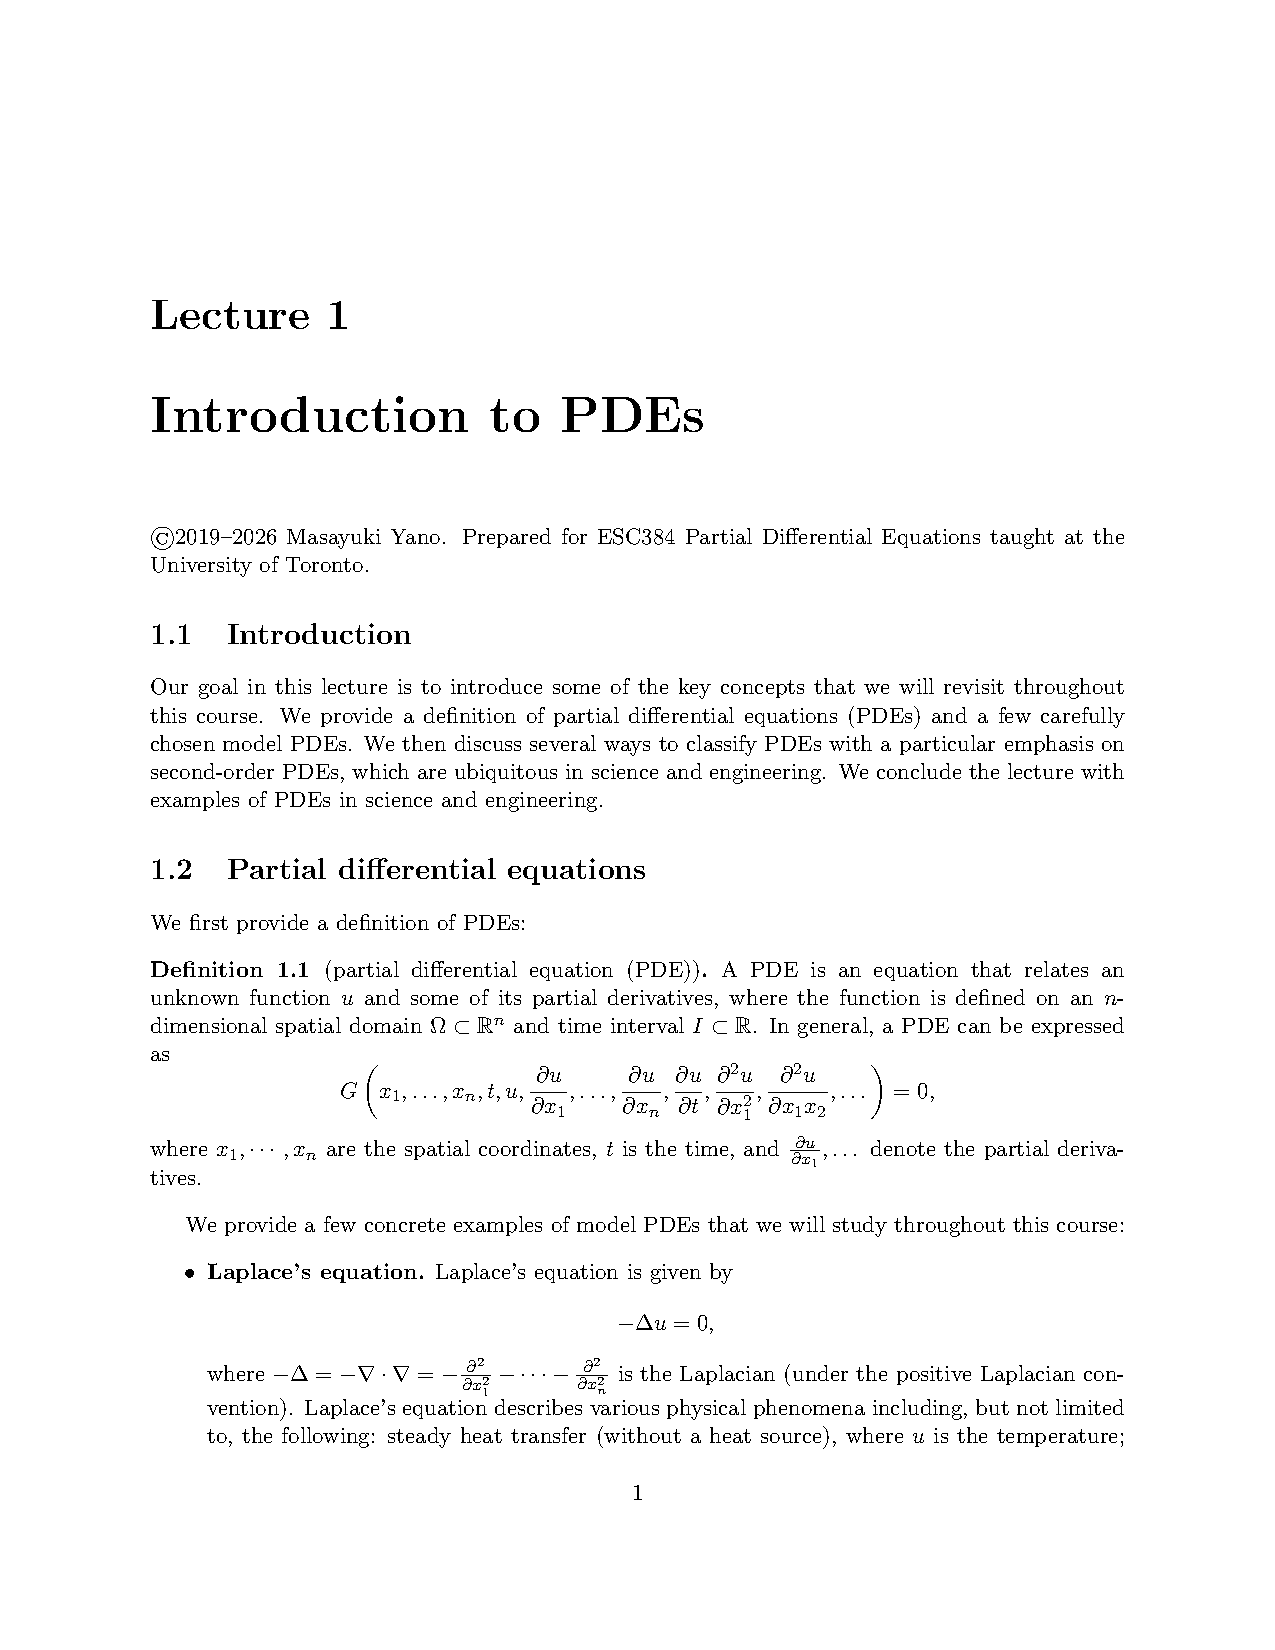
\includepdf[pages=-,addtotoc={1,section,1,{Lecture 1: Introduction to PDEs},lecpdf1}]{lectures/intro.pdf}
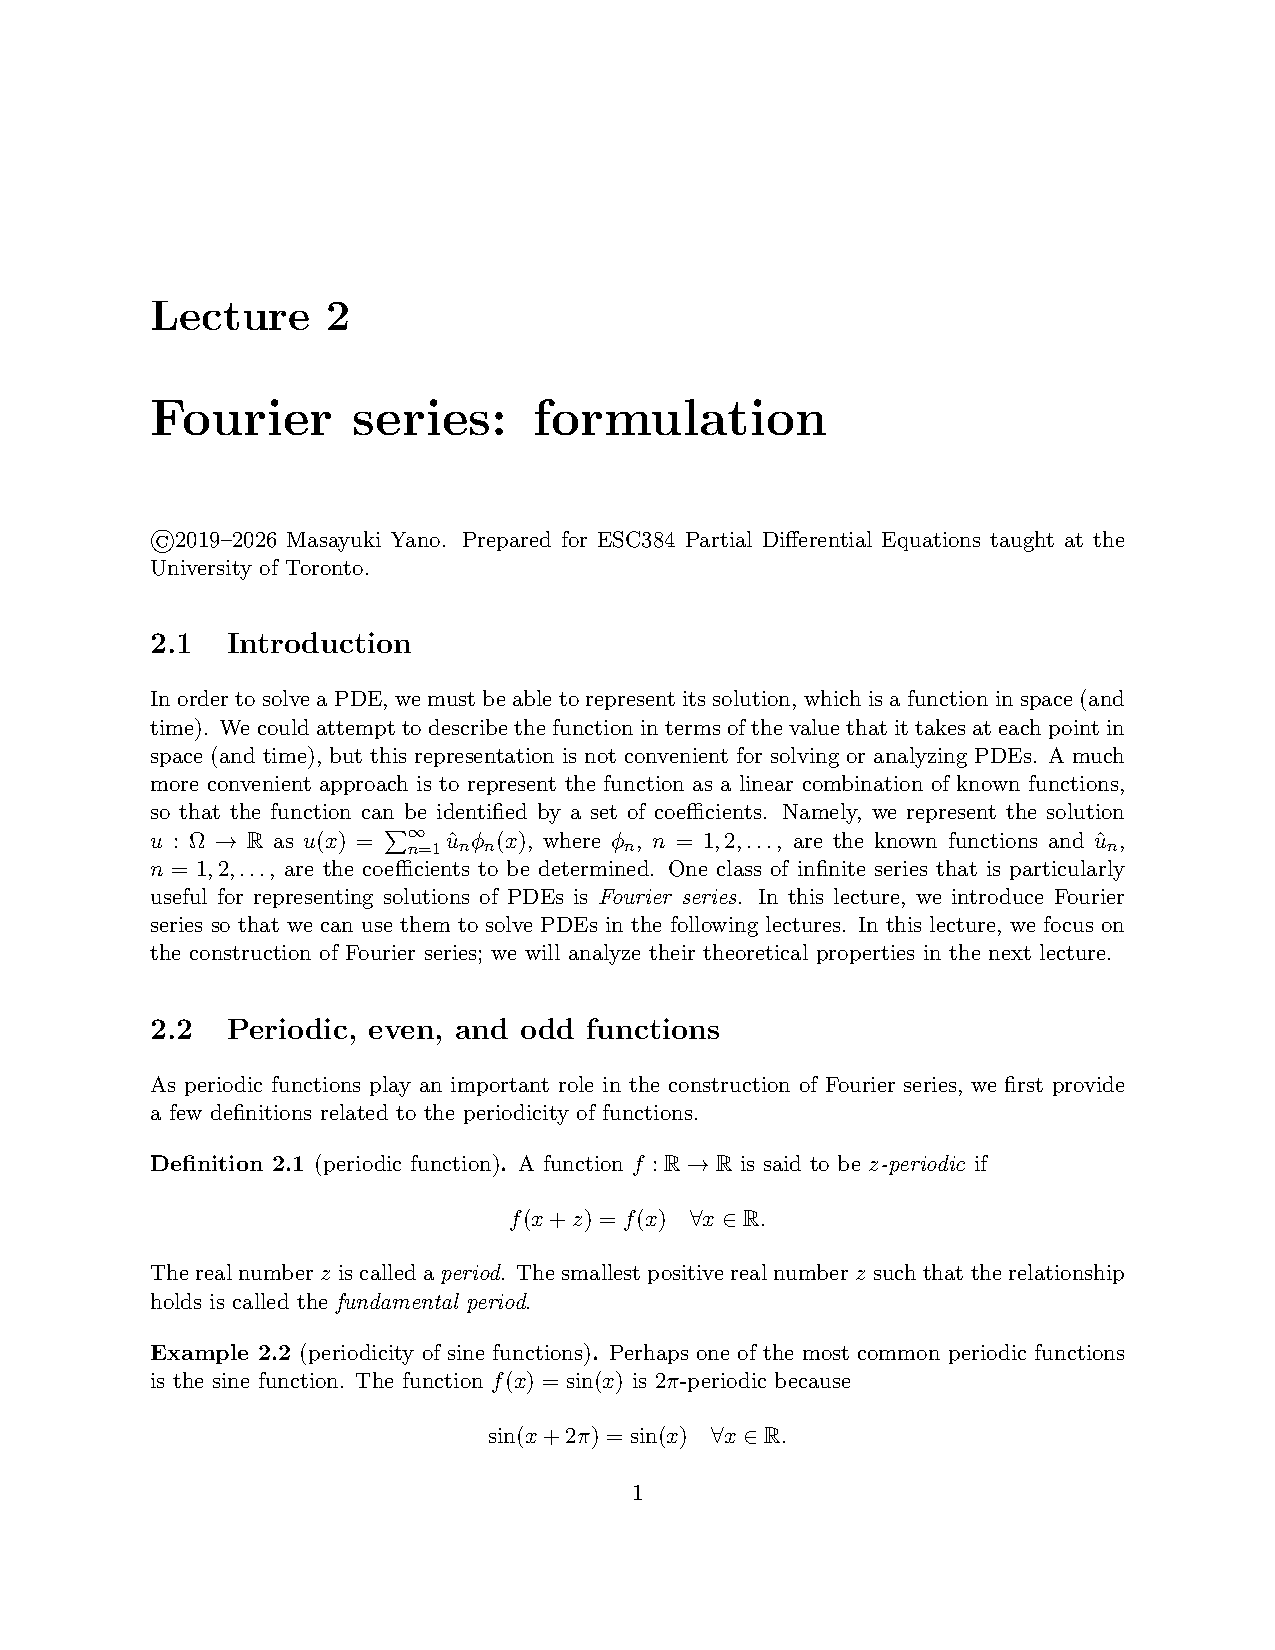
\includepdf[pages=-,addtotoc={1,section,1,{Lecture 2: Fourier series: formulation},lecpdf2}]{lectures/fourier_series.pdf}
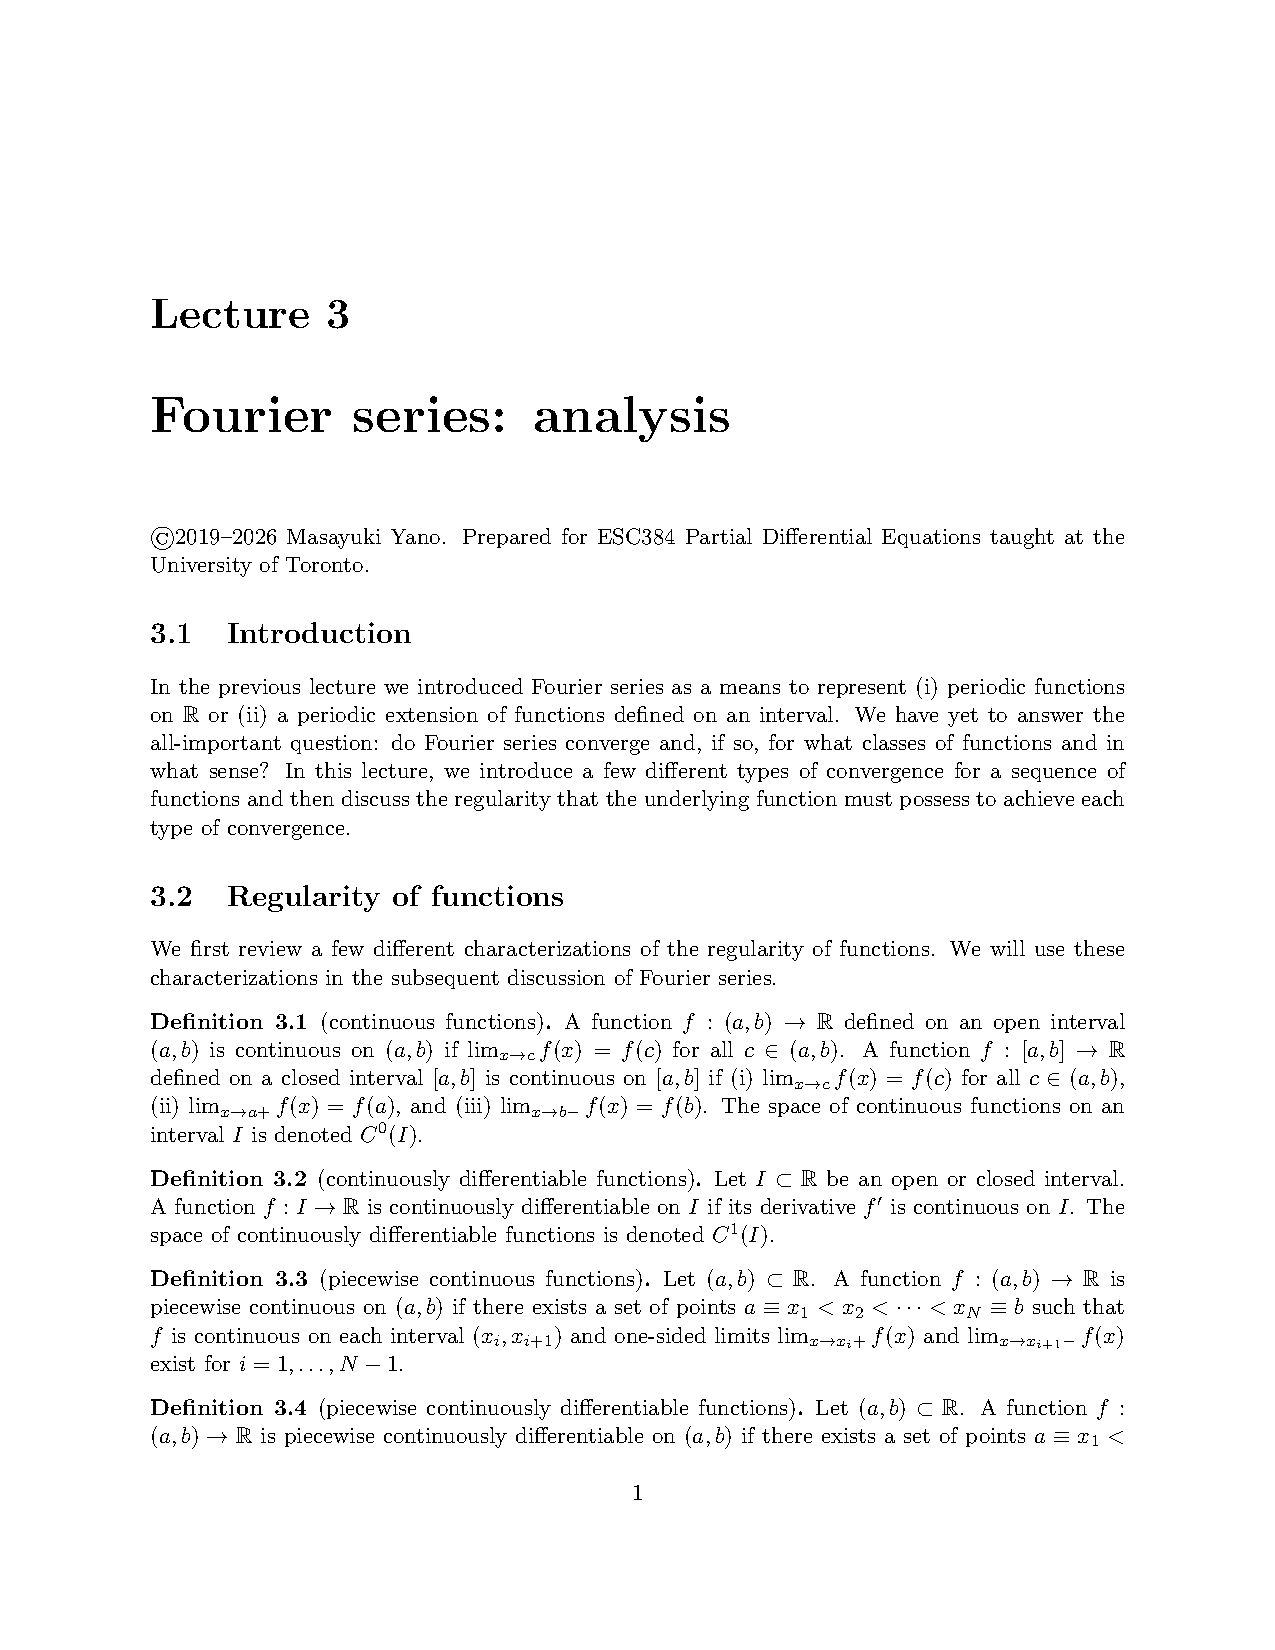
\includepdf[pages=-,addtotoc={1,section,1,{Lecture 3: Fourier series: analysis},lecpdf3}]{lectures/fourier_series_analysis.pdf}
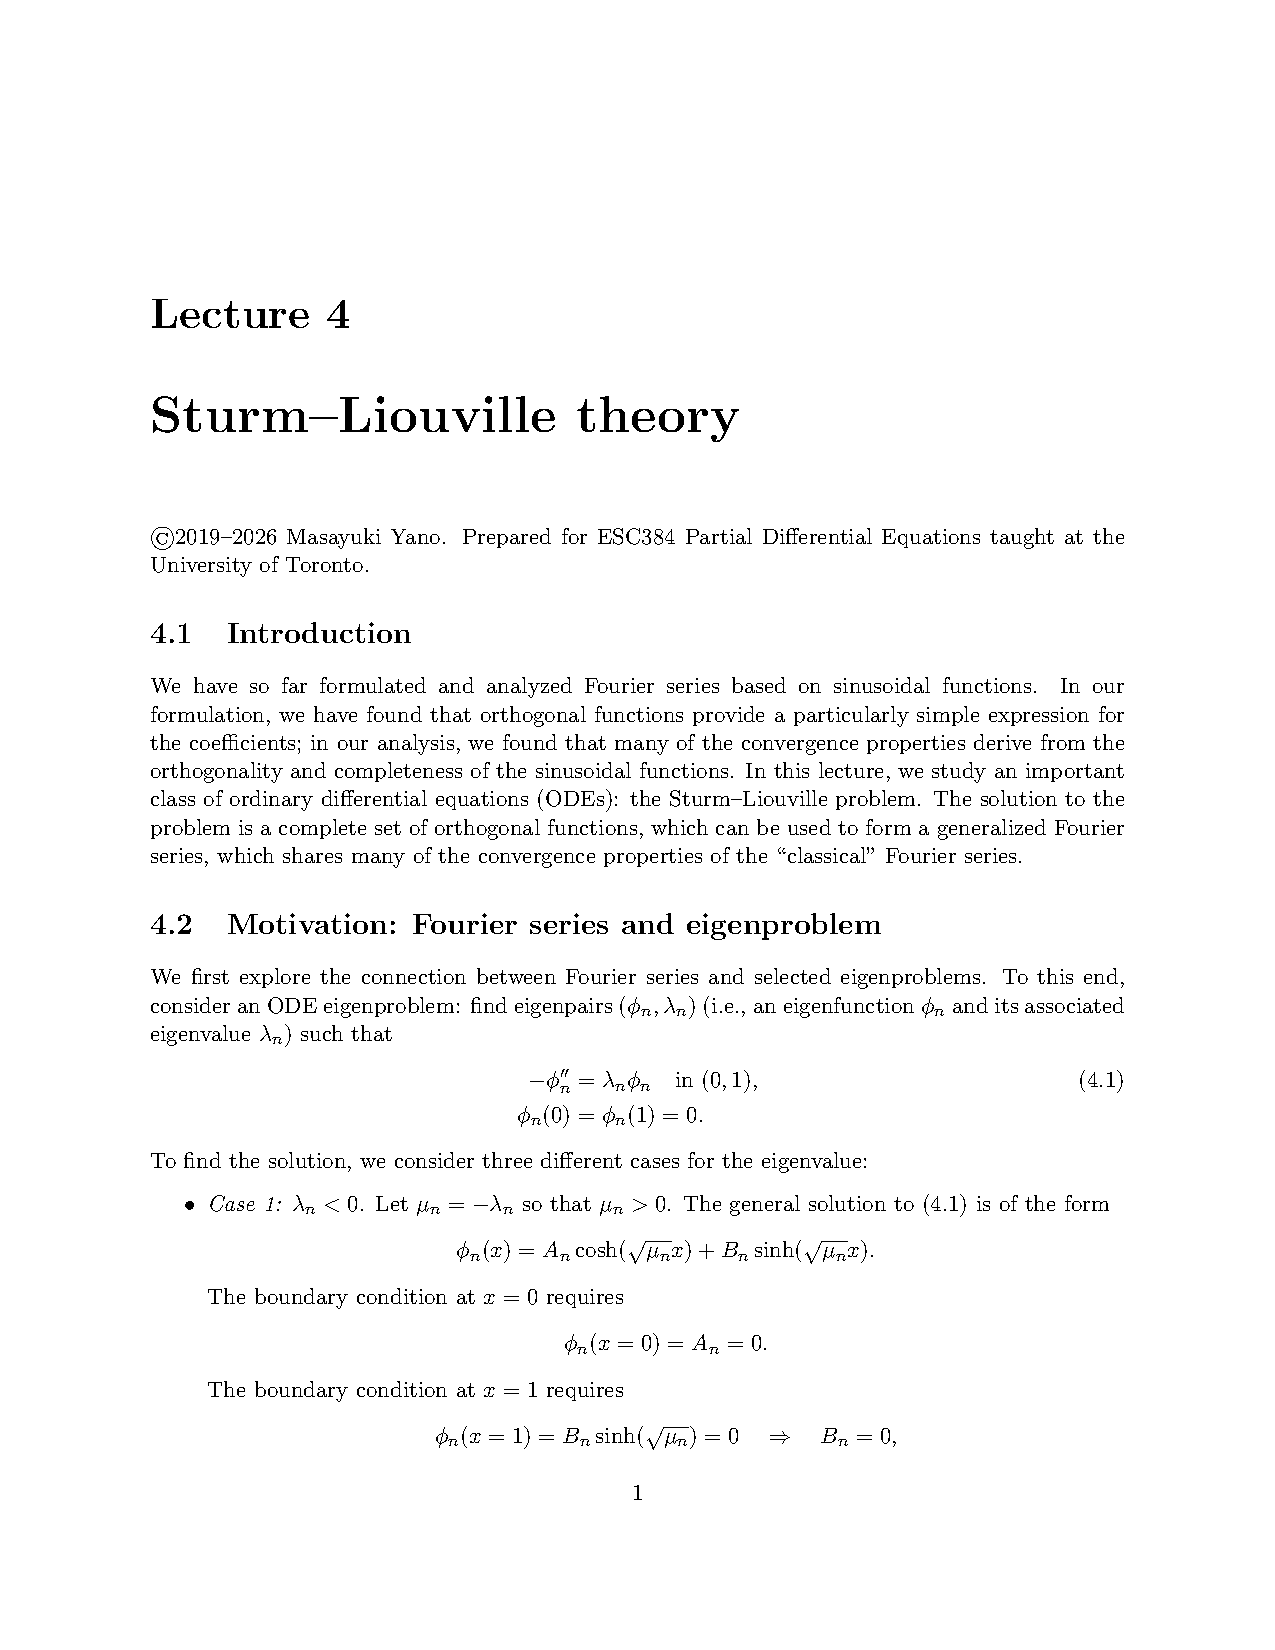
\includepdf[pages=-,addtotoc={1,section,1,{Lecture 4: Sturm–Liouville theory},lecpdf4}]{lectures/sturm_liouville.pdf}
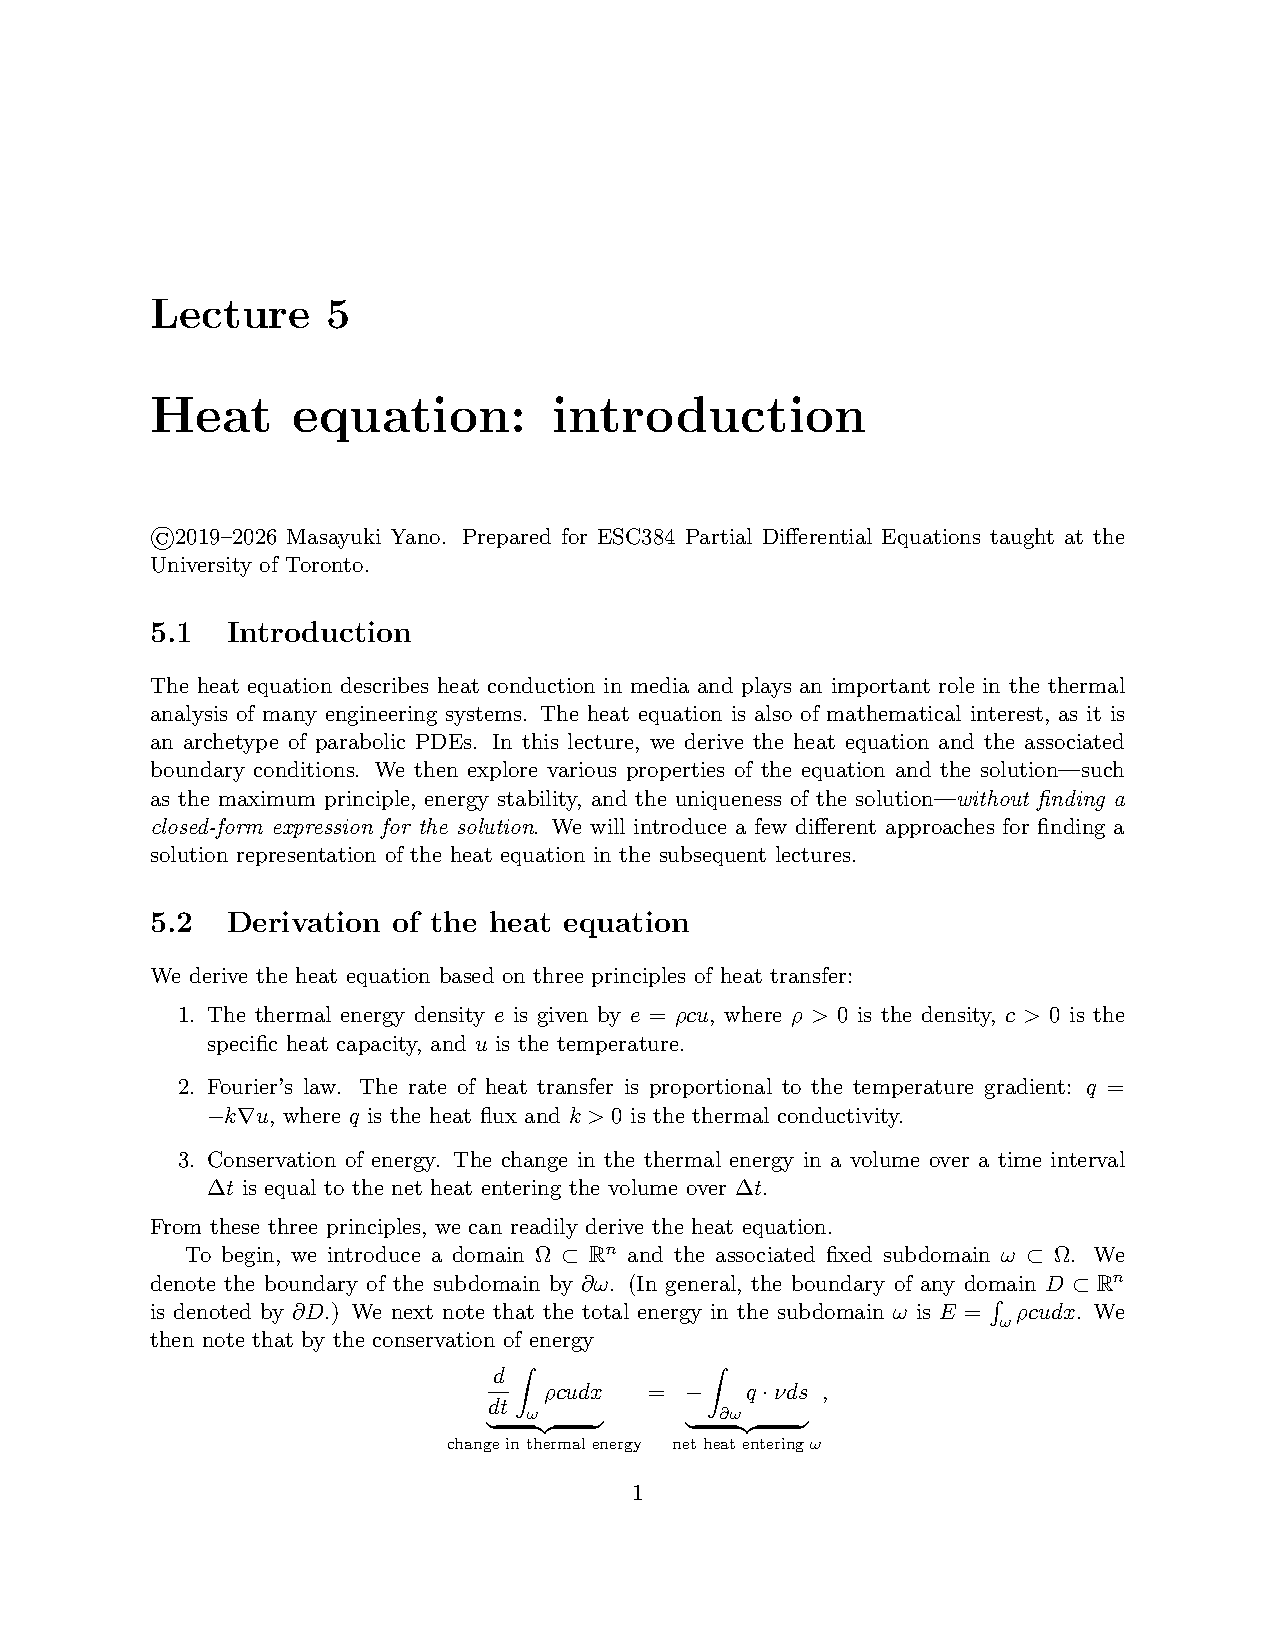
\includepdf[pages=-,addtotoc={1,section,1,{Lecture 5: Heat equation: introduction},lecpdf5}]{lectures/heat.pdf}
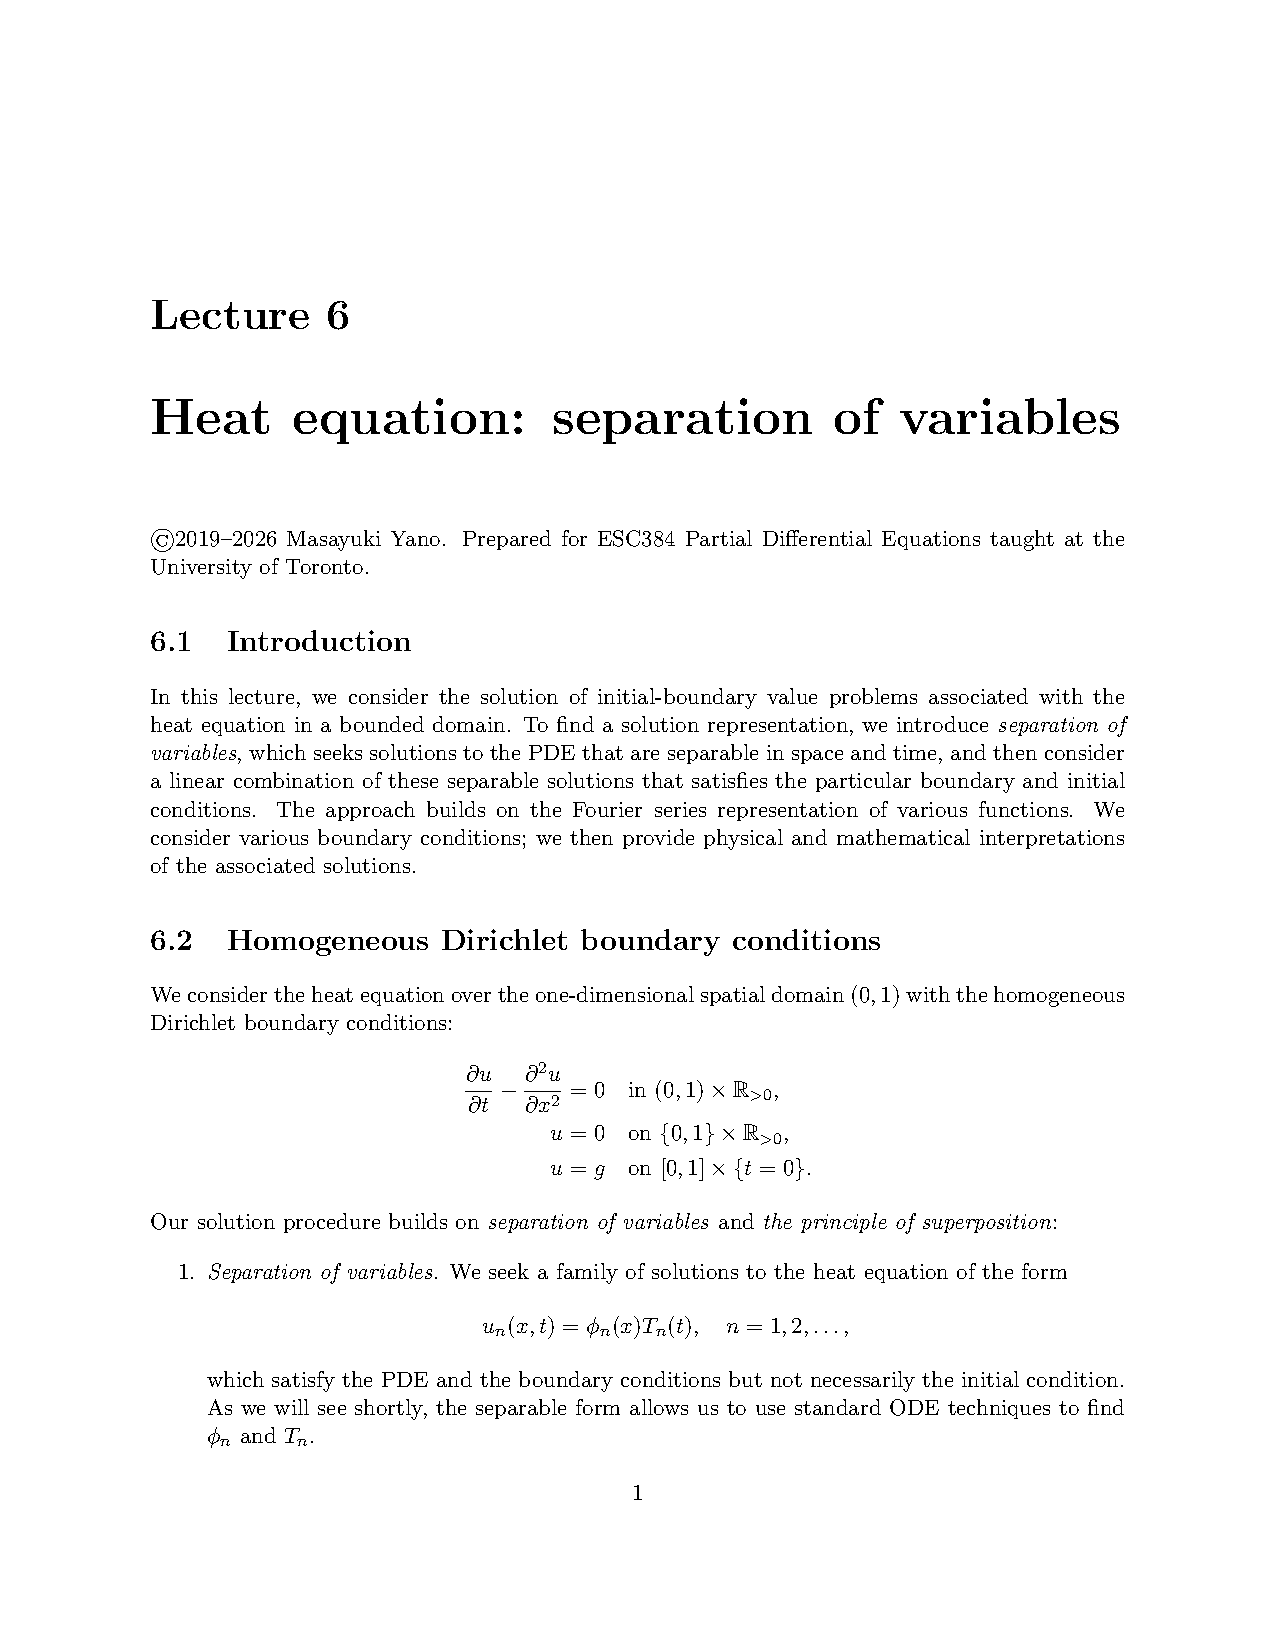
\includepdf[pages=-,addtotoc={1,section,1,{Lecture 6: Heat equation: separation of variables},lecpdf6}]{lectures/heat_sov.pdf}
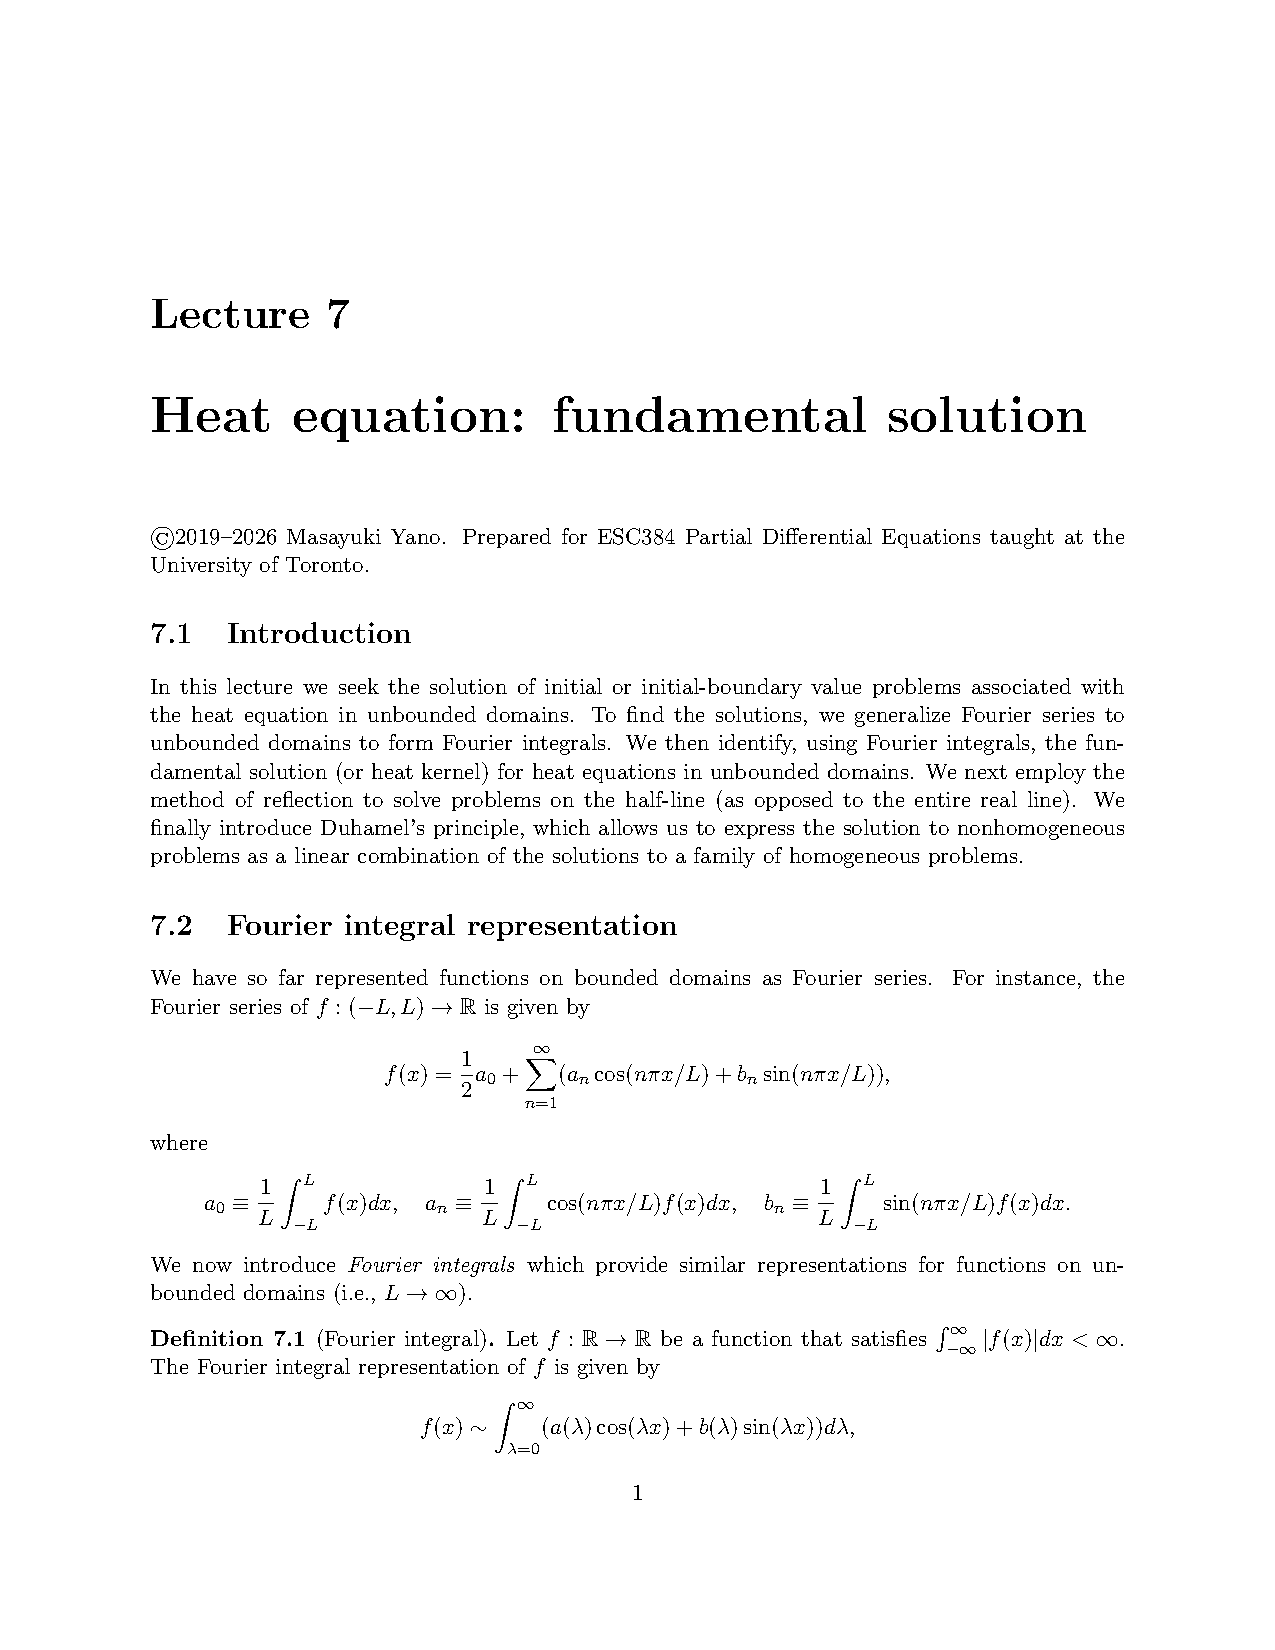
\includepdf[pages=-,addtotoc={1,section,1,{Lecture 7: Heat equation: fundamental solution},lecpdf7}]{lectures/heat_funsoln.pdf}
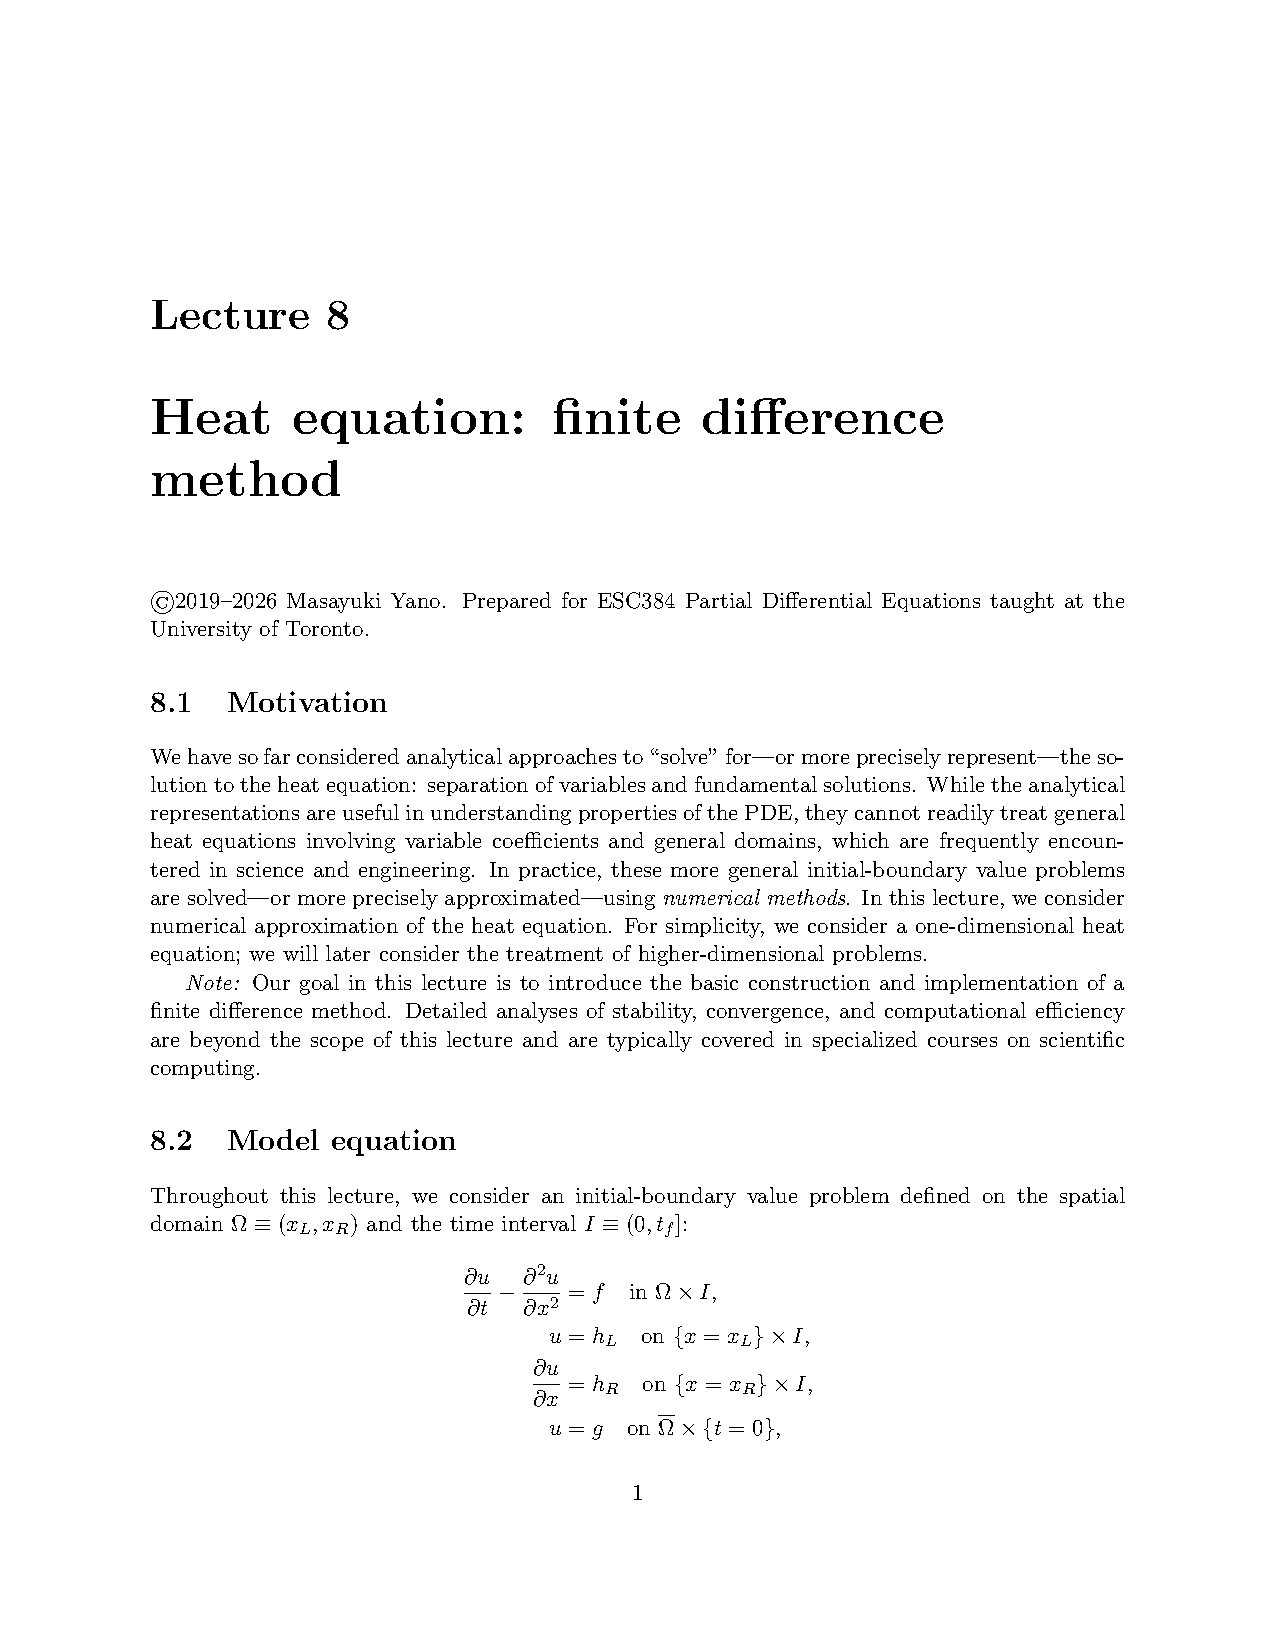
\includepdf[pages=-,addtotoc={1,section,1,{Lecture 8: Heat equation: finite difference method},lecpdf8}]{lectures/heat_fd.pdf}


% Previous typed notes (not currently included):
% % !TeX root = ../main.tex

% Edit this title for each week's entry.
\section{Unit 1:}
\newlecture[Introductions to PDEs][September 11, 2026]

\begin{definition}
    A PDE is an equation that relates an unkown function $u$ aNd some of its partial derivatives.
    \begin{center}
        \resizebox{\textwidth}{!}{$
            G\Big(\underbrace{x_1, \dots, x_n}_{\text{spatial coordinates}},\ \underbrace{t}_{\text{time}},\ \underbrace{u}_{\text{function}},\ \underbrace{\frac{\partial u}{\partial x_1}, \dots, \frac{\partial u}{\partial x_n}}_{\text{1st derivatives in space}},\ \underbrace{\frac{\partial u}{\partial t}}_{\text{1st derivatives in time}},\ \underbrace{\frac{\partial^2 u}{\partial x_1^2}, \frac{\partial^2 u}{\partial x_1 \partial x_2}, \dots}_{\text{2nd derivatives}}\Big) = 0
        $}
    \end{center}
\end{definition}

\begin{example}
    Model PDEs for this course.
    \\Laplace's Equation:
    \[-\Delta u = 0\]
    \[\text{Laplacian: }-\nabla \cdot \nabla = -\frac{\partial^2}{\partial x_1^2}-\frac{\partial^2}{\partial x_2^2} \text{ in }\mathbb{R}^2 \]
    Physics: potential flow, electrostatics, steady heat transfer...
\end{example}
Poisson's Equation:
\[-\Delta u = f \longleftarrow  \text{ source function: e.g. heat}\]

Heat Equation:
\[\frac{\partial u}{\partial t} - \Delta u = f \quad \text{physics: unsteady heat transfer, diffusion of chemicals...}\]
Transport Equation:
\[\frac{\partial u}{\partial t} + \underbrace{b}_{\text{advection field}} \cdot \nabla u = f \quad \text{physics: transport of conserved quantities}\]

Wave Equation:
\[\frac{\partial^2 u}{\partial t^2} - \underbrace{c^2}_{c: \text{ wave speed}} \Delta u = 0 \quad \text{physics: accousitics, vibration...}\]

Burger's Equation:
\[\frac{\partial u}{\partial t} + u\frac{\partial u}{\partial x} = 0 \quad \text{physics: nonlinear waves...}\]


\subsection{Classification of PDEs}
\begin{definition}
    The \textbf{order} of a PDE is the order of the highest derivative.
\end{definition}
\begin{example}
    \begin{align*}
        \text{Laplace's:} &\quad -\frac{\partial^2 u}{\partial x_1^2} - \frac{\partial^2 u}{\partial x_2^2} = 0 \quad \rightarrow \text{2nd order} \\
        \text{Transport:} &\quad \frac{\partial u}{\partial t} + \frac{\partial u}{\partial x} = 0 \quad \rightarrow \text{1st order} \\
        \text{Heat:} &\quad \frac{\partial u}{\partial t} - \Delta u = 0 \quad \rightarrow \text{2nd order (1st in time, 2nd in space)}
    \end{align*}
\end{example}

\begin{definition}
    An operator $\mathcal{L}$  is a \textbf{linear operator} if
    \[\mathcal{L} (\alpha w + \beta w) = \alpha \mathcal{L}  w + \beta \mathcal{L}  v\]
    for any functions $w$ \& $v$ and scalars $\alpha$ \& $\beta$
\end{definition}

\begin{definition}
    A PDE is \textbf{linear} if it can be expressed as
    \[\underbrace{\mathcal{L}}_{\text{linear operator}} u = \underbrace{f}_{\text{function independent of $u$}}\]
    If PDE is not linear, then it is a \underline{nonlinear PDE}.
\end{definition}

\begin{definition}
    A \textbf{linear homogeneous PDE} is a PDE of the form
    \[\mathcal{L} u = 0\]
    If a linear PDE is not homogeneous, then it is a \underline{linear nonhomogeneous PDE}.
\end{definition}

\begin{example}
    \begin{align*}
        \text{Laplace's:} &\quad -\Delta u =0 \quad \rightarrow \text{linear homogeneous} \\
        \text{Poisson's:} &\quad -\Delta u = f, f\neq 0 \quad \rightarrow \text{linear nonhomogeneous} \\
        \text{Heat:} &\quad \frac{\partial u}{\partial t} - \Delta u = 0 \quad \rightarrow \text{linear homogeneous}\\
        \text{Burger's:} &\frac{\partial u}{\partial t} + u \frac{\partial u}{\partial x} = 0 \quad \rightarrow \text{nonlinear}        
    \end{align*}
\end{example}

\subsection{Superposition}
\begin{itemize}
    \item If $\mathcal{L} u_1 = 0$ and $\mathcal{L} u_2 = 0$, then $\mathcal{L}(u_1+u_2)=0 $
    \item In addition, if $\mathcal{L} u_0 = f$, then $\mathcal{L}(u_0+u_1+u_2) = f$
\end{itemize}
\begin{itemize}[label = $\Rightarrow$]
    \item used frequently to solve \underline{linear} PDEs
    \item an unique solution found by imposing boundary (and initial) conditions
\end{itemize}

\subsection{Classification of Second-Order PDEs}
\begin{itemize}
    \item Consider a general linear operator of the form
    \[\mathcal{L} u = \sum_{i,j=1}^{n}a_{ij} \frac{\partial^2 u}{\partial x_i \partial y_i}+\sum_{i=1}^{n}b_i \frac{\partial u}{\partial x_i}+ cu\]
    (if problem is time-dependent, treat $t$ as 0-th coordinate)
    \item Let $A \in \mathbb{R} ^{n \times n}$ be a symmetric matrix s.t. $A_{ij} = a_{ij}$
    \item Let $\lambda_1, \dots, \lambda_n$ be the eigenvalues of $A$.
    \item Classifications:
    \begin{itemize}
        \item \textbf{elliptic}: all eigenvalues are nonzero and have same sign 
        \item \textbf{hyperbolic}: all eigenvalues are nonzero and exactly one of them have a different sibling
        \item \textbf{parabolic}: exactly one eigenvvalue is 0 and all others have the same sign
    \end{itemize}
\end{itemize}


\begin{example}

    Laplace's: $\mathcal{L} = -\Delta = -\frac{\partial^2}{\partial x_1^2} - \frac{\partial^2}{\partial x_2^2}$ in $\mathbb{R}^2$
    \[A = \begin{pmatrix} -1 & 0 \\ 0 & -1 \end{pmatrix} \quad \Rightarrow \lambda_1 = \lambda_2 = -1 \Rightarrow \text{ elliptic}\]

    Poisson's: elliptic

    Wave: $\mathcal{L} = \frac{\partial^2}{\partial t^2} - \Delta = \frac{\partial^2}{\partial t^2}- \frac{\partial^2}{\partial x_1^2} - \frac{\partial^2}{\partial x_2^2}$ (in $\mathbb{R}^2 \times \mathbb{R}$)
    \[A = \begin{pmatrix}
        1 & & \\ & -1 & \\ & & -1
    \end{pmatrix} \Rightarrow \lambda_1 = 1, \lambda_2 = \lambda_3 = -1 \Rightarrow \text{ hyperbolic}\]

    Heat: $\mathcal{L} = \frac{\partial}{\partial t} - \Delta = \frac{\partial}{\partial t} - \frac{\partial ^2}{\partial x_1^2} - \frac{\partial^2}{\partial x_2^2}$ in $\mathbb{R}^2 \times \mathbb{R} $
    \[A = \begin{pmatrix}
    0 & & \\ & -1 & \\ & & -1
    \end{pmatrix} \Rightarrow \lambda_1 = 0, \lambda_2 = \lambda_3 = -1 \Rightarrow \text{ parabolic}\]
\end{example}

\subsection{Variable Coefficient}
\[x_2 \frac{\partial ^2 u}{\partial x_1} + \frac{\partial ^2 u}{\partial x_2} = 0 \Rightarrow A = \begin{pmatrix}
    x_2 & 0 \\ 0 & 1
\end{pmatrix} \Rightarrow \lambda_1 = x_2, \lambda_2 = 1\]

\begin{center}
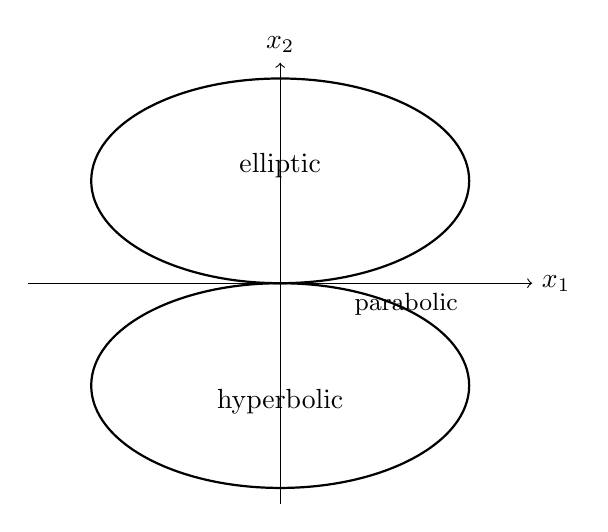
\begin{tikzpicture}[scale=1]
    \draw[->] (-3.2,0) -- (3.2,0) node[right] {$x_1$};
    \draw[->] (0,-2.8) -- (0,2.8) node[above] {$x_2$};

    \draw[thick] (0,1.3) ellipse (2.4cm and 1.3cm);
    \node at (0,1.5) {elliptic};

    \draw[thick] (0,-1.3) ellipse (2.4cm and 1.3cm);
    \node at (0,-1.5) {hyperbolic};

    \node[below] at (1.6,0) {\small parabolic};
\end{tikzpicture}
\end{center}


\newlecture[Fourier Series][September 14, 2026]
Motivation: to solve PDEs, we must represent solution $u$ as a function of space.

Given some function:
\begin{itemize}[label = ]
    \item Approach 1: describe point-wise values
    \item Approach 2: linear combination of known functions (e.g. polynomial)
    \[u(x) = \sum_{n=1}^{\infty} \hat{u}_n \varphi_n (x)\]
    $\Rightarrow$ can be easily differentiated: $u'(x) = \sum_{n=1}^{\infty}\hat{u}_n \varphi_n'(x)$
    $\Rightarrow$ classical method \underline{Fourier Series} (sin \& cos)
\end{itemize}

\begin{definition}
    $f: \mathbb{R} \rightarrow \mathbb{R} $ is \underline{$z$-periodic} if
    \[f(x+z) = f(x) \forall x \in \mathbb{R} \]
    \underline{Fundamental Period}: smallest $z$ for which the relationship holds
\end{definition}

\begin{example}
    \[f(x) = sin(x) \quad \Rightarrow \quad 2\pi \text{ periodic}\]
    \[f(x) = sin(x) + cos(2x) \quad \Rightarrow \quad 2\pi \text{ periodic}\]
\end{example}

\begin{definition}
    \(f:{ \mathbb{R} \rightarrow \mathbb{R}}\) is \underline{even} if $f(-x) = f(x)$, sym about y
    \(f: {\mathbb{R} \rightarrow \mathbb{R}}\) is \underline{odd} if $f(-x) = -f(x)$, sym about origin.
\end{definition}

\begin{definition}
    Given $f:(0, a) \rightarrow \mathbb{R}$, its \underline{periodic extension} to $\mathbb{R} $ is $f^p: \mathbb{R} \rightarrow \mathbb{R}$ such that $f^p(x) = f(x), x \in(0,a)$ and has a period of "$a$".
\end{definition}

\begin{definition}
    Given $f:(0, a) \rightarrow \mathbb{R}$, its \underline{even periodic extension} to $\mathbb{R} $ is $f^{e,p}: \mathbb{R} \rightarrow \mathbb{R}$ such that
    \[
    f^{e,p}(x) = \begin{cases}
        f(x), & x \in (0,a) \\
        f(-x), & x\in(-a, 0)
    \end{cases} \quad \text{and has a period of } 2a
    \]
\end{definition}

\begin{definition}
    Given $f:(0, a) \rightarrow \mathbb{R}$, its \underline{odd periodic extension} to $\mathbb{R} $ is $f^{o,p}: \mathbb{R} \rightarrow \mathbb{R}$ such that
    \[
    f^{o,p}(x) = \begin{cases}
        f(x), & x \in (0,a) \\
        -f(-x), & x\in(-a, 0)
    \end{cases} \quad \text{and has a period of } 2a
    \]
\end{definition}

\begin{definition}
    Let $f:\mathbb{R} \rightarrow \mathbb{R}$ be a 2-periodic function, the \rb{Fourier Series} of $f$ is
    \[f(x) ~ \frac{1}{2}a_0 + \sum_{n=1}^{\infty}(a_n cos (n\pi x) + b_n sin(n\pi x))\]
    with \underline{Fourier Coefficients}
    \[a_n = \int_{-1}^{1}cos(n \pi x)f(x)\,dx, \quad n=0,1,2,\dots\]
    \[b_ = \int_{-1}^{1}sin(n\pi x)f(x)  \,dx, \quad n = 1,2,3,\dots \]
\end{definition}

\begin{definition}
    \textbf{Truncated Fourier Series} is the partial sum
    \[S_N(x) = \frac{1}{2}a_0 + \sum_{n=1}^{N}(a_n cos(n\pi x) + b_n (n\pi x))\]
\end{definition}
Observations
\begin{enumerate}
    \item In general, the Fourier series of $f$ is \underline{not} equal to $f$, and hence we use "~" instead of "=".
    \item The set of functions
    \[\left\{\frac{1}{\sqrt{2}}, \sin(\pi x), \cos (\pi x), \sin(2\pi x), \cos(2\pi x), \dots\right\}\]
    is \underline{orthanormal} with respect to the $L^2$ inner product
    \[(w, v) = \int_{-1}^{1}wv\,dx \quad w,v,\in \mathbb{R}^2, w\cdot v = 0\]
    For all $n,m = 1,2,3\dots$
    \begin{itemize}
        \item $\int_{-1}^{1} (\frac{1}{\sqrt{2}})(cos(m \pi x))\,dx = \frac{1}{\sqrt{2}m\pi}sin(m\pi x)|^1_{x=-1} = 0$
        \item $\int_{-1}^{1} sin (m\pi x)\,dx = 0$
        \item $\int_{-1}^{1} cos(n\pi x) cos(m\pi x)\,dx - \delta_{mn} = \begin{cases}
            1 & \text{if }m=n \\
            0& \text{otherwise}
        \end{cases}$
        \item $\int_{-1}^{1} sin(n\pi x)sin(m\pi x)\,dx = \delta_{mn}$
        \item $\int_{-1}^{1} sin(n\pi x)cos(m\pi x)\,dx = 0$
    \end{itemize}
    \item Expression for Fourier coefficients are a consequence of orthogonality
    e.g. consider $a_2$
    \\ \underline{want}: $f(x) = \frac{1}{2}a_0 + \sum_{n=1}^{\infty} (a_n cos (n \pi x) + b_n sin(n\pi x))$
    \\ multiply by $cos(2\pi x)$ and integrate over $(-1,1)$
    \[\int_{-1}^{1}cos(2\pi x)f(x)  \,dx = \int_{-1}^{1}cos(2\pi x)[\frac{1}{2}a_0 + \sum_{n=1}^{\infty} (a_n cos (n\pi x) + b_n sin(n\pi x))]  \,dx  \]
    \[ = a_0 \underbrace{\int_{-1}^{1} \frac{1}{2}cos(2\pi x) \,dx }_{0} + \sum_{n=1}^{\infty} a_n \underbrace{a_n \int_{-1}^{1} cos(2\pi x)cos(n \pi x) \,dx }_{S_{n2}} + \sum_{n=1}^{\infty}\underbrace{\int_{-1}^{1} cos(2\pi x)sin(n \pi x) \,dx }_{=0}\]
    \[ = \sum_{n=1}^{\infty} a_n S_{n2} = a_2\]
    \item If $f:(-1, 1) \rightarrow \mathbb{R}$, then its Fourier series is "equal to"
    \begin{enumerate}[label = (\roman*)]
        \item $f$ as $(-1,1)$
        \item its periodic extension $f^p$ in $\mathbb{R}$
    \end{enumerate}
\end{enumerate}
\begin{example}
    \[f(x) = x \text{ for } x \in (-1,1)\]
    want: $f(x)\sim \frac{1}{2}a_0 +\sum_{n=1}^{\infty} (a_n cos(n\pi x) + b_n sin(n\pi x))$
    \[a_n = \int_{-1}^{1}f(x)cos(n\pi x)  \,dx = \int_{-1}^{1} x cos(n\pi x) \,dx =0\]
    \[b_n = \int_{-1}^{1}xsin(n\pi x)  \,dx = [\frac{sin(n\pi x)}{n^2 \pi^2}]|^1_{x=-1} - [\frac{xcos(n\pi x)}{n\pi}]|^1_{x=-1}\]
    \[-1 = -2\frac{cos(n\pi)}{n\pi}= -\frac{2(-1)^n}{n\pi} = 2\frac{(-1)^{n+1}}{n\pi}\]
    Hence, 
    \[f(x) \sim \sum_{n=1}^{\infty}b_n sin(n\pi x) = \boxed{\sum_{n=1}^{\infty} 2\frac{(-1)^{n+1}}{n\pi}sin(n\pi x)}\]
\end{example}

\begin{definition}
    Let $f: \mathbb{R} \rightarrow\mathbb{R} $ be an \underline{even $z$-periodic} function. The \rb{Fourier cosine series} is
    \[f(x) \sim \frac{1}{2}\hat{f}_0 + \sum_{n=1}^{\infty} \hat{f}_n cos(n\pi x)\]
    where $\hat{f}_n = \int_{-1}^{1} cos(n\pi x)f(x) \,dx = 2\int_{0}^{1} cos(n\pi x)f(x)  \,dx  $
    
    Let $f: \mathbb{R} \rightarrow\mathbb{R} $ be an \underline{even $z$-periodic} function. The \rb{Fourier sine series} is
    \[f(x) \sim \sum_{n=1}^{\infty} \hat{f}_n cos(n\pi x)\]
    where $\hat{f}_n = \int_{-1}^{1} sin(n\pi x)f(x) \,dx = 2\int_{0}^{1}sin(n\pi)x f(x)  \,dx $
\end{definition}
Observations:
\begin{enumerate}
    \item If $f:(0,1) \rightarrow \mathbb{R}$, then its Fourier cosine/sine series is "equal to"
    \begin{enumerate}[label = (\roman*)]
        \item $f$ as $(0,1)$ \& its even/odd periodic extension as $\mathbb{R} $
    \end{enumerate}
    \item We use $\hat{f}_n$ to denote Fourier cosine/sine coefficients of $f$
\end{enumerate}
\begin{example}
    Fourier cosine series of $f(x) = x, x \in (0,1)$
    \[\hat{f}_0 = 2\int_{0}^{1} x \,dx =1 \]
    \[\hat{f}_n = 2\int_{0}^{1}cos(n\pi x)x  \,dx = \begin{cases}
        -\frac{4}{n\pi^2}, & n \text{ odd} \\
        0, & n \text{ even}
    \end{cases} \]
    \[f(x) \sim \frac{1}{2}\hat{f}_0 + \sum_{n=1}^{\infty} \hat{f}_n cos(n \pi x) = \frac{1}{2} + \sum_{n=1, n\in \text{odd}}^{\infty}(-\frac{4}{n^2\pi^2}) cos (n\pi x)\]
    \[= \frac{1}{2} + \sum_{k=1}^{\infty} - \frac{4}{(2k-1)^2 \pi^2} cos((2k-1)\pi x)\]
\end{example}
\begin{example}
    Fourier sine series of $f(x) = x, x\in(0,1)$
    \[\hat{f}_n = 2\int_{0}^{1}sin(n\pi x)  \,dx = \cdots = \frac{2}{n\pi}(-1)^{n_1} \]
    \[f(x) \sim \sum_{n=1}^{\infty} \hat{f}_n sin(n\pi x) = \sum_{n=1}^{\infty} \frac{2(-1)^(n+1)}{n\pi}sin(n\pi x)\]
\end{example}

\b{Obstructions}:
\begin{enumerate}
    \item Coefficients follow from orthogonality
    \[\frac{1}{L} \int_{-L}^{L}\sin(\frac{n\pi x}{L})\sin(\frac{m\pi x}{L})\, dx = \delta_{mn}, \quad \text{etc}\]
    \item Given $f:(-L, L) \to \mathbb{R}$, its Fourier serires converges to $2L$ - periodic extension on $\mathbb{R}$.
\end{enumerate}
% 
\newlecture[Fourier Series: Analysis][Sep 18, 2026]

\[f(x) \sim \frac{1}{2}a_0 + \sum_{n=1}^{\infty}(a_n \cos(n\pi x) + b_n \sin(n\pi x))\]
\[S_N (x) = \frac{1}{2}a_0 + \sum_{n=1}^{N} (a_c \cos (n\pi x) + b_n \sin (n\pi x))\]
Question: Does $S_N \to f$ as $N \to \infty$? In what sense? For what functions?

\subsection{Regularity of Functions}
\begin{definition}
    $f:(a, b) \to \mathbb{R} $ is \underline{continuous} on $(a,b)$ if $\lim_{x \to c}f(x) = f(c), \quad \forall c \in (a,b)$
\end{definition}
\begin{definition}
    $f:[a,b] \to \mathbb{R}$ is \underline{continuous} on $[a,b]$ if $\lim_{x \to c}f(x) = f(c), \quad \forall c \in (a,b)$ and
    \[\lim_{x \to a^+}f(x) = f(a) \quad \text{and}  \quad \lim_{x \to b^-}f(x) = f(b)  \]
\end{definition}
\begin{definition}
    $f:I\to \mathbb{R}$ is \underline{continuously differentiable} on $I$ if $f'$ is continuous on $I$.
\end{definition}

\begin{example}
    \[f(x) = \left\lvert x\right\rvert , \quad x\in (-1,1)\]
\end{example}
\begin{example}
    \[f(x) = \sqrt{x}, \quad x\in [0,1]\]

    % include diagrams here!!!!!!


\end{example}

\begin{definition}
    $f:(a, b) \to \mathbb{R}$ is \underline{piecewise continuous} on $(a, b)$ 
    \\if $\exists$ a set of points $a \equiv x_1 < x_2 < \cdots < x_N \equiv b$ s.t. $f$ is continuous on each $(x_i, x_{i+1}) $ and one-sided limits $\lim_{x \to x_i^+}f(x)$ and $\lim_{x\to x_{i+1}^-}f(x)$ exist.
\end{definition}

\begin{definition}
    $f:(a,b) \to \mathbb{R}$ is \underline{piecewise continuously differentiable} on $a(,b)$ if $f'$ is piecewise continuous.
\end{definition}

\subsection{Convergence of Fourier Series}
\begin{theorem}[Pointwise Convergence]
    Let $f$ be a piecewise continuously differentiable function with a period 2. Then, for any $x\in \mathbb{R}$
    \[S_N(x) \to \frac{1}{2}[f(x^-) + f(x^+)] \text{ as } N \to \infty\]
\end{theorem}

\begin{corollary}
    if $f$ is continuous at $x$, then $S_N(x) \to f(x)$
    \\if $f$ is \underline{not} continuous at $x$, then $S_N(x) \to$ avergae of one-sided limits.
\end{corollary}


\begin{theorem}[Uniform Convergence]
    Let $f$ be a \underline{continuous} and \underline{piecewise continuously differentiable} function with a period 2. Then
    \[\mathcal{E}_N = \max_{x\in \mathbb{R}}\left\lvert f(x) - S_N(x)\right\rvert \to 0 \text{ as } N \to \infty\]
\end{theorem}

If a series is uniformly convergent
\begin{enumerate}
    \item $S_N$ gives a good approximation to $f$ at \underline{all} points (to within $\mathcal{E}_N$)
    \item We can make $\mathcal{E}_N$ arbitrarily small by taking $N$ large
    \item $f$ must be continuous (cf. uniform limit thm)
    \item Fourier series is equal to $f$
    \[f(x) = \frac{1}{2}a_0 + \sum_{n=1}^{\infty}(a_n \cos (n\pi x) + b_n \sin(n\pi x))\]
\end{enumerate}

\begin{theorem}[$L^2$ Convergence]
    Let $f$ be a square integratable function with a period 2: i.e.
    \[\int_{-1}^{1}f(x)^2 \, dx < \infty\]
    then, 
    \[\int_{-1}^{1}(f(x) - S_N(x))^2\, dx \to 0 \text{ as } N\to \infty\]
\end{theorem}
\begin{example}
    \[f(x) = sgn(\sin(\pi x))\] 
    Pointwise convergent? $\rightarrow$ piecewise continuously differentiable? YES
    \\Uniform convergent? $\rightarrow$ continuous? NO
\end{example}

\begin{example}
    \[f(x) = \left\lvert x \right\rvert \]
\end{example}

\subsection{Convergence on Finite Intervals}
\begin{itemize}
    \item Fourier series converges pointwise/uniformly/$L^2$ if the appropriate periodic extension satisfies the required continuity \& differentiability conditions.
    \item \underline{Coveat}: even if $f:[-L, L] \to \mathbb{R}$ is continuous, periodic extension may not be continuous
\end{itemize}

\subsection{Endpoint Conditions for Continuity}
\begin{itemize}
    \item full: $f:[-L, L] \to \mathbb{R}, \quad f(-L^+) = f(L^-) $
    \item sine: $f:[0,L] \to \mathbb{R}, \quad f(0^+) = f(L^-) = 0$
    \item cosine: $f:[0, L] \to \mathbb{R}$, no additional requirements.
    \item "Jump" (if any) at endpoints determines the value of Fourier series @ endpoints.
\end{itemize}


\subsection{Uniform and Absolute Convergence}
\begin{theorem}
    Fourier series $f(x)\sim \frac{1}{2}a_ + \sum_{n=1}^{\infty} (a_n \cos(n\pi x) + b_n \sin(n \pi x))$ converges uniformly if
    \[\sum_{n=1}^{\infty} (\left\lvert a_n\right\rvert + \left\lvert b_n\right\rvert ) < \infty\]
\end{theorem}
\begin{example}
    \[f(x) = x, x\in(0,1)\]
    Fourier cosine series: $\hat{f}_n = \frac{2}{n^2 \pi^2} ((-1)^n -1)$
    \[\sum_{n=1}^{\infty} \left\lvert \hat{f}_n\right\rvert \leq \sum_{n=1}^{\infty} \frac{4}{n^2 \pi^2} < \infty \Rightarrow \text{ uniform conv.}\]
    Fourier sine series: $\hat{f}_n = \frac{2}{n\pi} (-1)^{n+1}$
    \[\sum_{n=1}^{\infty}\left\lvert \hat{f}_n\right\rvert = \sum_{n=1}^{\infty}\frac{2}{n\pi} \Rightarrow \text{ diverges } \Rightarrow \text{ may not uniformly converge}\]
\end{example}

\subsection{Differentiation of Fourier Series}
\begin{theorem}
    Let $f$ be a continuous periodic function with piecewise continuously differentiable $f'$.
    \\Then, the Fourier series of $f'$ is given by term-by-term differentiation:
    \[f(x) \sim \frac{1}{2}a_0 + \sum_{n=1}^{\infty}(a_n \cos(n\pi x)+b_n \sin(n\pi x))\]
    \[f'(x) \sim \sum_{n=1}^{\infty} (-a_n n\pi x \sin(n\pi x)+ b_n n\pi x\cos (n\pi x))\]
\end{theorem}

\begin{theorem}[Uniform Convergence of Derivatives]
    The $k$-th derivative of $f$ is continuous if
    \[\sum_{n=1}^{\infty}(\left\lvert n^k a_n\right\rvert + \left\lvert n^k b_n \right\rvert ) < \infty\]
\end{theorem}

\begin{example}
    \[f(x) = \sum_{n=1}^{\infty} \underbrace{\exp (-\lambda n)}_{b_n} \sin (n\pi x) \text{ for } \lambda > 0\]
    \[\sum_{n=1}^{\infty}n^k \left\lvert b_n\right\rvert = \sum_{n=1}^{\infty}n^k \exp(-\lambda n) < \infty \text{ for any }k \]
\end{example}


\newlecture[Sturn-Liouville Problems][09.21]
Fourier Series \& Eigenproblems
\begin{example}
    Find eigenfunctions $\phi_n$ and eigenvalues $\lambda_n$ s.t.
    \[\begin{cases*}
        - \phi_n'' = \lambda_n \phi_n \text{ in } (0,1) &\text{ODE} \\
        \phi_n(x=0) = \phi_n(x=1) = 0 &\text{BCs}
    \end{cases*}\]

    Case 1: $\lambda_n <0 $
    \begin{quote}
    {   Let $\mu_n = -\lambda_n$ so that $\mu_n > 0$
        \\General solution to ODE: $\phi_n'' = \mu_n \phi_n$
        \[\phi_n = A_n' \exp(\sqrt{\mu_n}x)+B_n' \exp(-\sqrt{\mu_n}x)\]
        \[=A_n \cosh(\sqrt{\mu_n}x)+B_n \sinh(\sqrt{\mu_n}x)\]
        Recall: $\cosh(x) = \frac{1}{2}(e^x+e^{-x}), \sinh(x) = \frac{1}{2}(e^x - e^{-x})$
        \[\phi_n''(x) = A_n \mu_n \cosh(\sqrt{\mu_n}x) + B_n \mu_n \sinh(\sqrt{\mu_n} x) = \mu_n \phi_n\] 
        BC \@ $x=0: \quad \phi_n(x=0) = A_n \cosh(0) + B_n\sinh(0) = A_n = 0 \Rightarrow A_n = 0$ \\
        BC \@ $x=1: \quad \phi_n(x=1) = B_n \sinh(1) = 0 \Rightarrow B_n = 0$
        \\$\Rightarrow$ only solution is the trivial soulution $\phi_n = 0$} 
    \end{quote}

    Case 2: $\lambda_n = 0$
    \begin{quote}
        ODE: $-\phi_n '' = 0 \quad \Rightarrow \quad \phi_n(x) = A_n x+B+n$
        \\BC \@ $x=0: \quad \phi_n(x=0) = B_n = 0 \Rightarrow B_n = 0$
        \\BC \@ $x+1: \quad \phi_n(x=1) = A_n = 0 \Rightarrow A_n = 0$
        \\$Rightarrow$ only trivial solution $\phi_n = 0$
    \end{quote}


    Case 3: $\lambda_n > 0$
    \begin{quote}
        ODE: $-\phi_n'' = \lambda_n\phi_n$
        \[\Rightarrow phi_n(x) = A_n \cos (\sqrt{\lambda_n}x)+ B_n\sin(\sqrt{\lambda_n}x)\]
        BC \@ $x=0: \quad \phi_n(x=0) = A_n \cos(0)+ B_n\sin(0) = A_n = 0 \Rightarrow A_n=0$ \\
        BC \@ $x=1: \quad \phi_n(x=1) = B_n\sin(\sqrt{\lambda_n} \cdot 1) = 0$
        \begin{itemize}[label = $\Rightarrow$]
            \item since we want nontrivial solution, take $B_n \neq 0$
            \item $\sin(\sqrt{\lambda_n}) = 0 \Rightarrow \sqrt{(\lambda_n)} = n\pi \Rightarrow \lambda_n = n^2\pi^2, n = 1,2,3,\dots$
        \end{itemize}
        $\Rightarrow \phi_n(x) = \sin(n\pi x) \& \lambda_n = n^2\pi^2$ are the (nontrivial) solutions ot the eigenproblem.
    \end{quote}
\end{example}

\header{Observations}
\begin{enumerate}
    \item Eigenfunctions for the basis of Fourier sine series.
    $\hookrightarrow$ they can be used to approcimate functions
    \item Eigenfunctions are orthogonal
    \item Eigenvalues are real and non-negative
    \underline{Q.} could we have known this just by looking at the eigenproblem?
    \\\underline{Intuition}: eigenpairs of symmetric matrices
\end{enumerate}

\heading{Sturm-Liouville Theory}
\begin{definition}
    \b{Sturm-Liouville problem} is an eigenproblem of the form
    \[\begin{cases*}
        (p\phi')'+q\phi = \lambda w \phi \quad \text{in }(a,b) & \quad \text{ODE} \\
        \alpha_1 \phi(a) - \alpha_2 \phi'(a) = 0 & \quad \text{left BC} \\
        \beta_1 \phi(b) + \beta_2 \phi'(b) = 0 & \quad \text{right BC}
    \end{cases*}\]
    where:
    \begin{enumerate}[label = (\roman*)]
        \item $p, p'm q, \& w$ are continuous functions on $[a,b]$.
        \item $p>0 \& w > 0$ on $[a,b]$
        \item $\alpha_1^2 + \alpha_2^2 > 0$
        \item $\beta^2_1 + \beta_2^2 > 0$
    \end{enumerate}
\end{definition}

\begin{example}
    \[\begin{cases*}
        -\phi'' = \lambda\phi &\text{ in }(0,1)\\
        \phi(0) = \phi(1) = 0 &
    \end{cases*} \]
    is Sturm-Liouville problem with $p=1, q=0; w = 1, \alpha_1 = 1, \alpha_2 = 0, \beta_1 = 1, \beta_2 = 2$
\end{example}

\begin{theorem}
    Sturm-Liouville operator $L = -\frac{d}{dx}(p \frac{d}{dx}) + q$
    \\is \underline{self-adjoint}: i.e, 
    \[(Lw, v )= (w,Lv)\]
    for any continuously twice differentiablle functions $w \& v$ 
    \\when $(f,g)= \int_{a}^{b} f \bar{g}\,dx \quad$ for $\bar{g}$ is the complex conjugate.

    \b{Analogy}: if $A$ is symmetric, then
    \[(Aw, v) - v^TAw = w^T A^T v = w^T Av = (w, Av)\]
\end{theorem}


\begin{theorem}
    All eigenvalues of S-L problems are real.
    
    \b{Analogy}: all eigenvalues of symmetric $A$ are real.
\end{theorem}
\begin{theorem}
    Eigenfuncctions of S-L problems associated with distinct eigenvalues $\lambda_n \& \lambda_m$ are orthogonal wrt weight w:
    \[\int_{a}^{b} w\phi_n \phi_m\, dx = 0, \quad \forall n\neq m\]

    \b{Analogy}: eigenvectors of symmetric $A$ associated with distinct eigenvalues are orthogonal.
\end{theorem}

\begin{theorem}
    S-L problem has an infinite number of eigenvalues and $\lambda_n \to \infty$ as $n\to \infty$.
\end{theorem}
\begin{theorem}
    If $q\geq 0, \alpha_1 \geq 0, \alpha_2 \geq 0, \beta_1 \geq 0 \& \beta_2 \geq 0$, 
    \\then $\lambda_n \geq 0 \quad \forall n$
\end{theorem}

\b{Key}: given 
\[\begin{cases*}
    -\phi_n '' = \lambda_n\phi_n \quad &\text{in }(0,1) \\
    \phi_n(0) = \phi_n(1) = 0 &
\end{cases*}\]
we could have known, without knowing the solutions
\begin{enumerate}[label = \roman*]
    \item eigenfunctions are orthogonal
    \item eigenvalues are real \& non-negative
\end{enumerate}

\begin{example}
    \[\begin{cases*}
        -\phi'' = \lambda\phi \quad \text{in }(0,1) & \text{ODE} \\
        \phi'(0) = \phi'(1) = 0 &\text{BCs}
    \end{cases*}\]
    S-L problem with $p=1, q=0, w=1, \alpha_1 = \beta_1 = 0, \alpha_2 = \beta_2 = 1$
    \\$Rightarrow$ eigenfunctions are orthogonal; eigenvalues are real \& non-negative.

    Explicit Solution:
    \\Case 1: $\lambda = 0$ (note: we need \underline{not} consider $\lambda< 0$ by S-L theory)
    \begin{quote}
        \[\text{ODE: }-\phi_n'' = 0 \quad \Rightarrow \quad \phi_n(x) = A_n(x)+ B_n\]
        BC \@ $x=0: \quad \phi_n'(0) = A_n = 0 \quad \Rightarrow \quad A_n = 0$
        \\BC \@ $x=1: \quad \phi_n'(1) = A_n = 0$
        \[ \Rightarrow \text{pick }B_n = 1 \quad \Rightarrow \quad \phi_n(x = 1), \lambda_n = 0\]
    \end{quote}
    Case 2: $\lambda_n > 0$
    \begin{quote}
        \[\text{ODE: } -\phi_n'' = \lambda_n \phi_n \quad  \Rightarrow \quad \phi_n(x) = A_n\cos(\sqrt{\lambda_n}x) + B_n \sin(\sqrt{\lambda_n}x)\]
        BC \@ $x=0: \quad \phi_n'(0) = -A_n \sqrt{\lambda_n}\sin(\sqrt{\lambda_n}\cdot 0)+ B_n \sqrt{\lambda_n} \cos(\sqrt{\lambda_n}\cdot 0) = 0 \Rightarrow B_n = 0$
        \\BC \@ $x=1: \quad \phi_n'(1) = -A_n \sqrt{\lambda_n}\sin(\sqrt{\lambda_n}\cdot 1) = 0 \Rightarrow \sin(\sqrt{\lambda_n}) = 0\Rightarrow \lambda_n = n^2\pi^2, n = 1,2,\dots$
    \end{quote}

    \[\phi_n(x) = \begin{cases*}
        1, &n=0 \\
        \cos(n\pi x), &n=1,2,3, \dots
    \end{cases*} = \cos(n\pi x), n = 0,1,2, \dots \]
    \[\lambda_n = \begin{cases*}
        0, &n=0 \\
        n^2\pi^2, &n=1,2,3,\dots
    \end{cases*} = n^2\pi^2, n=0,1,2,\dots \Rightarrow \text{Fourier cosine series}\]
\end{example}

\header{Generalized Fourier Series}
Let $(\phi_n)^{\infty}_{n=1}$ be eigenfunctions of the S-L problem with $\alpha_1, \alpha_2, \beta_1, \beta_2 \geq 0$.
\\We can approximate any square integrable $f: (a, b) \to \mathbb{R}$ by generalized Fourier series.
\[f(x) \sim \sum_{n=1}^{\infty}\hat{f}_n\phi_n(x)\]
where 
\[\hat{f_n} = \frac{\int_{a}^{b} f(x)\phi_n (x)w(x)\, dx}{\int_{a}^{b}\phi_n(x)^2w(x)\, dx}\]
note: the basis is orthogonal, not necessarily orthanormal.

\header{Remarks}:
\begin{enumerate}
    \item Coefficients follow from orthogonality
    \item Series converges point-wise/uniformaly/in $L^2$ given a sufficiently regular $f$.
\end{enumerate}



\end{document}
